\documentclass[11pt]{elegantbook}
\usepackage{graphicx}
\usepackage{float}
\definecolor{structurecolor}{RGB}{40,58,129}
\linespread{1.6}
\setlength{\footskip}{20pt}
\setlength{\parindent}{0pt}
\newcommand{\argmax}{\operatornamewithlimits{argmax}}
\newcommand{\argmin}{\operatornamewithlimits{argmin}}
\elegantnewtheorem{proof}{Proof}{}{Proof}
\elegantnewtheorem{claim}{Claim}{prostyle}{Claim}
\DeclareMathOperator{\col}{col}
\title{Regression and Estimation}
\author{Wenxiao Yang}
\institute{Haas School of Business, University of California Berkeley}
\date{2023}
\setcounter{tocdepth}{2}
\extrainfo{All models are wrong, but some are useful.}

\cover{cover.png}

% modify the color in the middle of titlepage
\definecolor{customcolor}{RGB}{32,178,170}
\colorlet{coverlinecolor}{customcolor}
\usepackage{cprotect}

\addbibresource[location=local]{reference.bib} % bib

\begin{document}
\maketitle

\frontmatter
\tableofcontents

\mainmatter


\chapter{Statistics Basics}
\textbf{\underline{Objective}:} Using $x$ to give (data-based) answers to questions about the distribution of $X$, i.e., $P_0$.

\textbf{\underline{Probability vs. Statistics}:}
\begin{enumerate}[$\circ$]
    \item Probability: Distribution known, outcome unknown;
    \item Statistics: Distribution unknown, outcome known.
\end{enumerate}

\textbf{\underline{Setting:}} $X_1,...,X_n$ is a random sample from a discrete/continuous distribution with pmf/pdf $f(\cdot\mid \theta)$, where $\theta\in\Theta$ is unknown.

\textbf{\underbar{Types of Statistical Inference}:}
\begin{enumerate}[$\circ$]
    \item Point estimation $\Rightarrow$ "What is $\theta$?";
    \item Hypothesis testing $\Rightarrow$ "Is $\theta=\theta_0$?";
    \item Interval estimation $\Rightarrow$ "Which values of $\theta$ are 'plausible'?".
\end{enumerate}

\begin{example}
    \underline{Examples of Statistical Models}
    \begin{enumerate}[(1).]
        \item $x_i\sim \text{i.i.d. } \text{Bernoulli}(p)$, where $p$ is unknown.
        \item $x_i\sim \text{i.i.d. } U(0,\theta)$, where $\theta>0$ is unknown.
        \item $x_i\sim \text{i.i.d. } N(\mu,\sigma^2)$, where $\mu\in \mathbb{R}$ and $\sigma^2>0$ are unknown.
    \end{enumerate}
\end{example}
\section{Random Sampling}
\begin{definition}[Random Sample]
    \normalfont
    A \textbf{random sample} is a collection $X_1,...,X_n$ of random variables that are (mutually) independent and identical marginal distributions.

    $X_1,...,X_n$ are called "independent and identically distributed". The notation is $X_i\sim i.i.d. $
\end{definition}

\begin{definition}[Statistic]
    \normalfont
    A \textbf{statistic} (singular) or sample statistic is any quantity computed from values in a sample which is considered for a statistical purpose.\\
    If $X_1,...,X_n$ is a random sample and $T: \mathbb{R}^n \rightarrow \mathbb{R}^k$ (for some $k\in \mathbb{N}$), then $T(X_1,...,X_n)$ is called a \textbf{statistic}.
\end{definition}

\subsection{Sample Mean and Sample Variance}
\begin{definition}[Sample Mean and Sample Variance]
    \normalfont
    \begin{enumerate}
        \item The \textbf{sample mean} is $\bar{X}=\frac{1}{n}\sum_{i=1}^n X_i$;
        \item The \textbf{sample variance} is $S^2=\frac{1}{n-1}\sum_{i=1}^n (X_i-\bar{X})^2=\frac{1}{n-1}(\sum_{i=1}^n X_i^2 - n\bar{X}^2)$
    \end{enumerate}
\end{definition}

\begin{note}
    We use "$X_i\sim \text{i.i.d}(\mu,\sigma^2)$" to denote a random sample from a distribution with mean $\mu$ and variance $\sigma^2$.
\end{note}

\begin{theorem}[$\mathbb{E}(\bar{X}), \text{Var}(\bar{X}), \mathbb{E}(S^2)$]
    Suppose $X_1,...,X_n$ is a random sample from a distribution with mean $\mu$ and variance $\sigma^2$ (denoted by $X_i\sim \text{i.i.d}(\mu,\sigma^2)$). Then,
    \begin{enumerate}[(a).]
        \item $\mathbb{E}(\bar{X})=\mu$;
        \item $\text{Var}(\bar{X})=\frac{\sigma^2}{n}$;
        \item $\mathbb{E}(S^2)=\sigma^2$.
    \end{enumerate}
\end{theorem}


\subsection{Distributional Properties}
\begin{theorem}
    If $X_i\sim \text{i.i.d. } N(\mu,\sigma^2)$, then
    \begin{enumerate}[(a).]
        \item $\bar{X}\sim \mathcal{N}(\mu,\frac{\sigma^2}{n})$
        \item $\frac{n-1}{\sigma^2}S^2\sim \chi^2_{n-1}$
        \item $\bar{X}\perp S^2$
    \end{enumerate}
\end{theorem}

\begin{theorem}["Asymptotics"]
    If $X_i\sim \text{i.i.d. } (\mu,\sigma^2)$ and if $n$ is "large", then
    \begin{enumerate}[(a).]
        \item $\bar{X}\sim \mathcal{N}(\mu,\frac{\sigma^2}{n})$ (converges in distribution) by CLT \ref{CLT};
        \item $S^2=\sigma^2$ by LLN;
    \end{enumerate}
\end{theorem}

\subsection{Order Statistics}
\begin{definition}[Order Statistics]
    \normalfont
    If $X_1,...,X_n$ is a random sample, then the \textbf{characteristics} are the sample values placed in ascending order.
    \underline{Notation:}
    \begin{equation}
        \begin{aligned}
            X_{(1)}\leq X_{(2)}\leq ... \leq X_{(n)}
        \end{aligned}
        \nonumber
    \end{equation}
\end{definition}

\begin{proposition}[Distribution of $X_{n}=\max_{i=1,...,n}X_i$]
    If $X_1,...,X_n$ is a random sample form a distribution with cdf $F$ (denoted by "$X_i\sim \text{i.i.d. } F$"), then
    \begin{equation}
        \begin{aligned}
            F_{X_{(n)}}(x)=P(X_{(n)}\leq x)=F^n(x)
        \end{aligned}
        \nonumber
    \end{equation}
\end{proposition}
\begin{proposition}[cdf and pdf]
    More generally,
    \begin{equation}
        \begin{aligned}
            F_{X_{(r)}}(x)&=\sum _{j=r}^{n}{\binom {n}{j}}[F_{X}(x)]^{j}[1-F_{X}(x)]^{n-j}\\
            f_{X_{(r)}}(x)&={\frac {n!}{(r-1)!(n-r)!}}f_{X}(x)[F_{X}(x)]^{r-1}[1-F_{X}(x)]^{n-r}
        \end{aligned}
        \nonumber
    \end{equation}
\end{proposition}
\begin{example}\quad
    \begin{enumerate}
        \item \textbf{Order statistics sampled from a uniform distribution on unit interval ($\text{Unif}[0,1]$):} Consider a random sample $U_1,...,U_n$ from the standard uniform distribution. Then,
        \begin{equation}
            \begin{aligned}
                f_{X_{(k)}}(x)&={\frac {n!}{(k-1)!(n-k)!}}u^{k-1}(1-u)^{n-k}
            \end{aligned}
            \nonumber
        \end{equation}
        The $k^{th}$ order statistic of the uniform distribution is a beta-distributed random variable. $$U_{(k)}\sim \text{Beta}(k,n+1-k)$$
        which has mean $\mathbb{E}[U_{(k)}]=\frac{k}{n+1}$.
        \item \textbf{The joint distribution of the order statistics of the uniform distribution on unit interval ($\text{Unif}[0,1]$):}
        Similarly, for $i < j$, the joint probability density function of the two order statistics $U_{(i)} < U_{(j)}$ can be shown to be
        \begin{equation}
            \begin{aligned}
                {\displaystyle f_{U_{(i)},U_{(j)}}(u,v)=n!{u^{i-1} \over (i-1)!}{(v-u)^{j-i-1} \over (j-i-1)!}{(1-v)^{n-j} \over (n-j)!}}
            \end{aligned}
            \nonumber
        \end{equation}
        The joint density of the $n$ order statistics turns out to be constant:
        \begin{equation}
            \begin{aligned}
                {\displaystyle f_{U_{(1)},U_{(2)},\ldots ,U_{(n)}}(u_{1},u_{2},\ldots ,u_{n})=n!}
            \end{aligned}
            \nonumber
        \end{equation}
        For $n\geq k>j\geq 1$, $U_{(k)}-U_{(j)}$ also has a beta distribution:
        \begin{equation}
            \begin{aligned}
                {\displaystyle U_{(k)}-U_{(j)}\sim \operatorname {Beta} (k-j,n-(k-j)+1)}
            \end{aligned}
            \nonumber
        \end{equation}
        which has mean $\mathbb{E}[U_{(k)}-U_{(j)}]=\frac{k-j}{n+1}$
    \end{enumerate}
\end{example}


\section{Statistics Model (ECON 240B)}
\subsection{Model}
A statistical model is a family of probability distributions over the data.

In statistics, we define \textit{data} be a vector $x=(x_1,...,x_n)'\in\Omega$ of numbers, where $x_i\in \mathbb{R}^d$. $x$ is the realization of a random vector $X=(X_1,...,X_n)'$. The $X$ follows a distribution $P_0$, which is the \textit{True Probability Generating Data (DGP)}. If $P_0$ is i.i.d., we have $P_0(X)=P_0(x_1)P(x_2)\cdots P_0(x_n)$.

\begin{definition}[Model]
    \normalfont
    A model $P\subseteq \{\text{Probabilities over }\Omega\}$ and a i.i.d. model $P\subseteq \{\text{Probabilities over }\mathbb{R}^d\}$.
\end{definition}

\begin{definition}[Well-Specified Model]
    \normalfont
    A model is \textbf{well-specified} if $P\ni P_0$.
\end{definition}

\subsection{Parametric Model}
\begin{definition}[Parametric Model]
    \normalfont
    A \underline{non-parametric} model $\bar{P}\cong \{\text{Probabilities over }\mathbb{R}^d\}$.\\
    A \underline{parametric} model $P=\{P_\theta:\theta\in\Theta\subseteq \mathbb{R}^v\}$.\\
    A \underline{semi-parametric} model: not parametric / non-parametric.
\end{definition}

\begin{example}
    \begin{enumerate}
        \item \underline{Parametric} model: $P=\{\Phi(\theta,1):\theta\in \mathbb{R}\}$, where $\Phi$ is the Gaussian c.d.f.
        \item Regression Models. $Z:=(Y,X)$. $P$ belongs to the model iff $\mathbb{E}_P[y^2]<\infty$ and $\mathbb{E}_P[XX^T]$ is non-singular and finite. The model gives $\mathbb{E}_P[Y|X]=h(X)$.
        \begin{enumerate}[(A).]
            \item \underline{Semi-parametric} model: $h\in\{\text{linear functions}\}$ i.e., $h(X)=\beta^TX$ for some $\beta\in \mathbb{R}^d$.
            \item \underline{Non-parametric} model: $h\in\{f:\mathbb{E}_p[f(x)^2]<\infty\}$.
        \end{enumerate}
    \end{enumerate}
\end{example}

\subsection{Parameter}
\begin{example}
    \underline{Potential Outcome Model}: $Z:=(Y,D,X)$, where $Y$ is the outcome, $D\in\{0,1\}$ is the treatment, and $X$ is the covariates.
    \begin{enumerate}[$\circ$]
        \item $P$ belongs to the model iff $(y_{(0)},y_{(1)})$ represents the potential outcome given different treatment $D\in\{0,1\}$, $y=Dy_{(1)}+(1-D)y_{(0)}$, and
        \item we study $e(x):=P(D=1|x)$.
        \item Average Treatment Effect (ATE) is given by $\text{ATE}_{P_0}:=\mathbb{E}_{P_0}[y_{(1)}-y_{(0)}]$, where $P_0$ is the DGP. It is impossible to estimate the ATE even if we have enough data, since $y_{(1)}$ and $y_{(0)}$ can't be observed at the same time. We need to link it to something we can estimate.
    \end{enumerate}
\end{example}



\begin{definition}[Parameter]
    \normalfont
    A parameter is a ``feature'' of $P_0$: $v(P), P\in \mathcal{P}$. Specifically, $v(P_0)$ is the true parameter of the DGP.
\end{definition}

\begin{example}
    \begin{enumerate}
        \item \underline{Linear Regression Model}: $\mathbb{E}_{P_0}[Y|X]=\beta^T_0 X$.\\
        We solve $\beta$ by $\min_\beta \mathbb{E}_{P_0}[(y-\beta^Tx)^2]$. The F.O.C. gives $\mathbb{E}_{P_0}[YX^T]=\beta^T \mathbb{E}_{P_0}[XX^T]$. $\beta_0$ solves this.
        \item \underline{Linear Instrumental Variable Model}: $\mathbb{E}_P[(Y-\beta^T_0X)|W]=0$, where $W$ is the instrumental variable. Look at $\mathbb{E}_{P_0}[(Y-\beta^TX)W]=0$. Consider an estimator $\hat{\beta}$,
        \begin{equation}
            \begin{aligned}
                0&=\mathbb{E}_{P_0}[(Y-\beta^TX)W]\\
                &=\mathbb{E}_{P_0}[(\hat{\beta}-\beta_0)^TXW]\\
                &=\underbrace{(\hat{\beta}-\beta_0)^T}_{1\times m}\underbrace{\mathbb{E}_{P_0}[XW]}_{m\times k}
            \end{aligned}
            \nonumber
        \end{equation}
        which holds iff $\hat{\beta}=\beta_0$ given $\mathbb{E}_{P_0}[XW]$ has full rank.
        \item \underline{Identification of the ATE in the Potential Outcomes Model}: To identify the ATE, we give two assumptions:
        \begin{equation}
            \begin{aligned}
                ATE:=\mathbb{E}[Y(1)-Y(0)]
            \end{aligned}
            \nonumber
        \end{equation}
        To identify the ATE, we give two assumptions:
        \begin{enumerate}
            \item A1 (Overlap): $e(X):=P(D=1|X)\in(0,1)$
            \item A2 (Unconfoundednes): $(Y(0),Y(1))\perp D|X$, i.e., $(Y(0),Y(1))$ are independent of $D$ given $X$.
        \end{enumerate}
        $\text{ATE}=\mathbb{E}[y(1)-y(0)]=\mathbb{E}[\mathbb{E}[y(1)|X]-\mathbb{E}[y(0)|X]]$. $\mathbb{E}[y|D=1,X]=\mathbb{E}[y(1)|D=1,X]$. Given Assumption A1: $y(1)\perp D|X$, $\mathbb{E}[y|D=1,X]=\mathbb{E}[y(1)|D=1,X]=\mathbb{E}[y(1)|X]$.
        \item \underline{Inference}: For a parameter $\theta(P_0)$, we have an estimate $\hat{\theta}_m$ (with sample size $m$), which has C.D.F. $v(P_0)$. For all $t\in \mathbb{R}$, the C.D.F. is given by
        \begin{equation}
            \begin{aligned}
                v(P_0)(t)=\textnormal{Pr}_{P_0}(\hat{\theta}_m-\theta(P_0)\leq t)
            \end{aligned}
            \nonumber
        \end{equation}
    \end{enumerate}
\end{example}

\section{Model Estimation (ECON 240B)}
\subsection{Plug-In Estimation}
For a model $P$, we have ``identification'' $v(P_0):=\theta_0$. How to estimate unknown $P_0$?

\begin{definition}[Empirical Probability/CDF]
    \normalfont
    Empirical probability/CDF: $$P_m(A)=\frac{1}{m}\sum_{i=1}^m \mathbf{1}\{Z_i\in A\}$$
    By the LLN, $P_m(A) \stackrel{P_0}{\longrightarrow} P_0(A)$.
\end{definition}

\begin{definition}[Plug-in estimator]
    \normalfont
    A \textbf{Plug-in estimator} is an estimator based on the empirical CDF, which is given by
    \begin{equation}
        \begin{aligned}
            \hat{\theta}_m=v(P_m)
        \end{aligned}
        \nonumber
    \end{equation}
    \underbar{Note:} The domain of $v$ is $\mathcal{P}$. Is $v(P_m)$ well-defined? It might be $P_m\notin \mathcal{P}$.
\end{definition}

\begin{example}
    \begin{enumerate}
        \item $\mathcal{P}=\{\text{all pdf with finite first moments}\}$. $v(P_0)=\mathbb{E}_{P_0}[Z]$, $v(P_m)=\frac{1}{m}\sum_{i=1}^m Z_i$.
        \item $\mathcal{P}$ is the set of linear regression models. $v(P_0)=\argmin_b \mathbb{E}_{P_0}[(Y-b^TX)^2]=\mathbb{E}_{P_0}[XX^T]^{-1}\mathbb{E}_{P_0}[XY]$,
        \begin{equation}
            \begin{aligned}
                v(P_m)=\mathbb{E}_{P_m}[(Y-b^TX)^2]=\argmin_b\frac{1}{m}\sum_{i=1}^m\left(Y_i-b^TX_i\right)^2=\left(\frac{1}{m}\sum_{i=1}^mX_iX_i^T\right)^{-1}\left(\frac{1}{m}\sum_{i=1}^mX_iY_i\right)
            \end{aligned}
            \nonumber
        \end{equation}
        where $v(P_m)$ is OLS.
        \item \textbf{GMM}. $\forall P\in \mathcal{P}: \mathbb{E}_P[g(Z,v(p))]=0$, where $g$ is a known moment function. $$v(P_0)=\argmin_\theta \mathbb{E}_{P_0}[g(Z,\theta)]^TW\mathbb{E}_{P_0}[g(Z,\theta)]$$
        where $W$ is a weighted matrix.
        \begin{equation}
            \begin{aligned}
                v(P_m)=\argmin_\theta \left(\frac{1}{m}\sum_{i=1}^m g(Z_i,\theta)\right)^TW\left(\frac{1}{m}\sum_{i=1}^m g(Z_i,\theta)\right)
            \end{aligned}
            \nonumber
        \end{equation}
        The $v(P_m)$ is the \textbf{Gaussian Estimator}.
        \item (When it doesn't work.) For the linear regression case, $v(P_m)=\underbrace{\left(\frac{1}{m}\sum_{i=1}^mX_iX_i^T\right)^{-1}}_\text{well-defined?}\left(\frac{1}{m}\sum_{i=1}^mX_iY_i\right)$. If the $\#$ of Covariates $> m$, the estimator is not well-defined.
        \item (When it doesn't work.) $\mathcal{P}$ is the potential outcome model. $\text{ATE}=v(P_0)=\mathbb{E}_{P_0}[\mu_1(x)-\mu_0(x)]$ where $\mu_d(x):=\mathbb{E}_{P_0}[y|D=d,x],d=0,1$.
        \begin{equation}
            \begin{aligned}
                v(P_m)=\frac{1}{m}\sum_{i=1}^m\left(\underbrace{\mathbb{E}_{P_m}[y|D=1,X_i]}_\text{well-defined?}-\mathbb{E}_{P_m}[y|D=0,X_i]\right)
            \end{aligned}
            \nonumber
        \end{equation}
        $\mathbb{E}_{P_m}[y|D=d,x]$ is ``too complex'' to define, (consider the example that $x$ is continuous).
    \end{enumerate}
\end{example}
\underline{What is the solution when the Plug-in estimation doesn't work?}
\begin{enumerate}
    \item Propose a functional form restriction $\mu_d$.
    \item ``Regularization'': Kernel estimators and series estimators.
\end{enumerate}


\subsection{Bootstrap}
Let $v(P_0)\text{ be the CDF of }\theta(P_m)-\theta(P_0)$, where $C(P_m,P_0):=\theta(P_m)-\theta(P_0)$.
\begin{equation}
    \begin{aligned}
        v(P_0)(t)=\textnormal{Pr}_{P_0}\left(C(P_m,P_0)\leq t\right),\forall t
    \end{aligned}
    \nonumber
\end{equation}
Here, the data $\{Z_i\}_i$ is generated from $P_0$, which forms $P_m$.

\begin{remark}
    Sometimes, instead of $C(P_m,P_0)$, we may study
    \begin{equation}
        \begin{aligned}
            v_A(P_0)(t)=\textnormal{Pr}_{P_0}\left(T(P_m,P_0)\leq t\right), \forall t
        \end{aligned}
        \nonumber
    \end{equation}
    where $T(P_m,P_0):=\frac{C(P_m,P_0)}{\sqrt{\text{Var}_{P_0}(\theta(P_m))}}$.
\end{remark}

\begin{definition}[Bootstrap Estimator]
    \normalfont
    The Plug-in estimator $v(P_m)$ is a.k.a. the \textbf{Bootstrap estimator}. Now, we generate new data i.i.d. from $P_m$, $\{Z_i^*\}_i \stackrel{i.i.d.}{\sim} P_m$, which forms $P_m^*$.
    \begin{equation}
        \begin{aligned}
            v(P_m)(t):=\textnormal{Pr}_{P_m}\left(\theta(P_m^*)-\theta(P_m)\leq t\right)
        \end{aligned}
        \nonumber
    \end{equation}
\end{definition}
\paragraph*{Computation of $v(P_m)$}
\begin{enumerate}[(1).]
    \item Draw $\{Z_i^*\}_i$ from $P_m$ and forms $P_m^*$.
    \item Based on the new $P_m^*$, compute $C^{(b)}(P_m^*,P_m)=\theta(P_m^*)-\theta(P_m)$.
    \item Repeat (1) and (2):
    \begin{equation}
        \begin{aligned}
            \frac{1}{B}\sum_{b=1}^B \mathbf{1}\{C^{(b)}(P_m^*,P_m)\leq t\}\stackrel{B \rightarrow \infty}{\longrightarrow}v(P_m)(t)
        \end{aligned}
        \nonumber
    \end{equation}
\end{enumerate}


\begin{example}[ (Sample Mean)]
    Consider $\theta(P_0)=\mathbb{E}_{P_0}(Z)$, then $\theta(P_m)=\bar{Z}_m=\frac{1}{m}\sum_{i=1}^m Z_i$. $v(P_0)(t)=\textnormal{Pr}_{P_0}\left(\frac{1}{m}\sum_{i=1}^m (Z_i-\mathbb{E}_{P_0}(Z))\leq t\right)$. The Bootstrap estimator is given by
    \begin{equation}
        \begin{aligned}
            v(P_m)(t)=\textnormal{Pr}_{P_m}\left(\frac{1}{m}\sum_{i=1}^m (Z_i^*-\bar{Z}_m)\leq t\right)
        \end{aligned}
        \nonumber
    \end{equation}
    or
    \begin{equation}
        \begin{aligned}
            v_A(P_m)(t)=\textnormal{Pr}_{P_m}\left(\sqrt{m}\frac{\frac{1}{m}\sum_{i=1}^m (Z_i^*-\bar{Z}_m)}{\sqrt{\text{Var}_{P_m}(\theta(P_m^*))}}\leq t\right)
        \end{aligned}
        \nonumber
    \end{equation}
    where $Z_i^*\sim_{i.i.d.} P_m$, $Z_i^*\in\{Z_1,...,Z_m\},\forall i\in\{1,...,m\}$. For the $v_A(P_0)$, $\text{Var}_{P_0}(\theta(P_m))=\frac{1}{m}\sigma^2_{P_0}(Z)$ and $\text{Var}_{P_m}(\theta(P_m^*))=\frac{1}{m}\sigma^2_{P_m}(Z)=\frac{1}{m}S^2_Z$, where $S_Z^2$ is the sample variance of $Z$.
    
    It is equivalent to give a weight to each $Z_i$, $\sum_{i=1}^m Z_i^*=\sum_{i=1}^m W_{i,m} Z_i$, where $$\left(W_{1,m},...,W_{m,m}\right)\sim\text{Multinomial}\left(\frac{1}{m},....,\frac{1}{m},m\right),\ W_{i,m}\in\{0,1,...,m\}$$
    Based on this, the Bootstrap estimator can be rewritten as
    \begin{equation}
        \begin{aligned}
            v(P_m)(t)=\textnormal{Pr}\left(\frac{1}{m}\sum_{i=1}^m (W_{i,m}-1)Z_i\leq t\right)
        \end{aligned}
        \nonumber
    \end{equation}
    (Other Bootstrap procedure, $W_{i,m}$ is not restricted to be multinomial, $\mathbb{E}[W_{i,m}]=1$.)
\end{example}


\subsubsection*{Consistency}
\begin{definition}[Consistency of Estimator]
    \normalfont
    The estimator $v(P_m)(t)$ is \textbf{consistent} if
    \begin{equation}
        \begin{aligned}
            \sup_t|v(P_m)(t)-v(P_0)(t)|=\underbrace{o_{P_0}(1)}_\text{Goes to zero in probability}
        \end{aligned}
        \tag{*}
        \label{consistency}
    \end{equation}
\end{definition}

\subsubsection*{Bootstrap Confidence Intervals}
\begin{definition}[$\tau$-th quantile]
    \normalfont
    Let $q_\tau(v(P))$ be the $\tau$-th quantile of $v(P)$:
    \begin{equation}
        \begin{aligned}
            q_\tau(v(P))=v(P)^{-1}(\tau),\ \tau\in(0,1)
        \end{aligned}
        \nonumber
    \end{equation}
\end{definition}

``Ideal'' Confidence Interval: Suppose you know $v(P_0)$, the ideal interval is $$CI^0_\alpha:=\left[\theta(P_m)-q_{1-\frac{\alpha}{2}}(v(P_0)),\theta(P_m)-q_{\frac{\alpha}{2}}(v(P_0))\right]$$
The confidence interval of the Bootstrap estimator is given by
\begin{equation}
    \begin{aligned}
        CI^\text{Bootstrap}_\alpha:=\left[\theta(P_m)-q_{1-\frac{\alpha}{2}}(v(P_m)),\theta(P_m)-q_{\frac{\alpha}{2}}(v(P_m))\right]
    \end{aligned}
    \nonumber
\end{equation}
\begin{theorem}
    Assuming the consistency of the Bootstrap estimator, the confidence interval of it satisfies
    \begin{equation}
        \begin{aligned}
            \textnormal{Pr}_{P_0}\left(CI^\text{Bootstrap}_\alpha\ni \theta(P_0)\right)\geq 1-\alpha+o_{P_0}(1)
        \end{aligned}
        \nonumber
    \end{equation}
\end{theorem}
\begin{proof}
    By \eqref{consistency}, we have
    \begin{equation}
        \begin{aligned}
            q_\tau(v(P_m))=q_\tau(v(P_0))+o_{P_0}(1)
        \end{aligned}
        \nonumber
    \end{equation}
    Then,
    \begin{equation}
        \begin{aligned}
            \textnormal{Pr}_{P_0}\left(CI^\text{Bootstrap}_\alpha\ni \theta(P_0)\right)&=\text{Pr}_{P_0}\left[\theta(P_m)-q_{1-\frac{\alpha}{2}}(v(P_m))\leq\theta(P_0)\leq\theta(P_m)-q_{\frac{\alpha}{2}}(v(P_m))\right]\\
            &=\text{Pr}_{P_0}\left[q_{1-\frac{\alpha}{2}}(v(P_m))\geq C(P_m,P_0)\geq q_{\frac{\alpha}{2}}(v(P_m))\right]\\
            &=v(P_0)\left(q_{1-\frac{\alpha}{2}}(v(P_m))\right)-v(P_0)\left(q_{\frac{\alpha}{2}}(v(P_m))\right)\\
            &=v(P_0)\left(q_{1-\frac{\alpha}{2}}(v(P_0))\right)-v(P_0)\left(q_{\frac{\alpha}{2}}(v(P_0))\right)+o_{P_0}(1)\\
            &=1-\alpha+o_{P_0}(1)
        \end{aligned}
        \nonumber
    \end{equation}
    The second last equality holds by \eqref{consistency} and continuity of the c.d.f. $v(P_0)$ (assumed).
\end{proof}
\begin{remark}
    \begin{enumerate}[(1).]
        \item Choice of quantiles:
        \begin{enumerate}
            \item If you impose symmetry at $0$: $-q_{1-\frac{\alpha}{2}}(v(P))=q_{\frac{\alpha}{2}}(v(P))$.
        \end{enumerate}
        \item P-values: the same idea of using confidence intervals. By the consistency and the continuity of the c.d.f. $v(P)$, the p-value converges to the true p-value.
        \item ``Bootstrap'' standard errors can't be used.
    \end{enumerate}
\begin{definition}[Bootstrap standard error]
    \normalfont
    The object of interest is $\sqrt{\text{Var}_{P_0}(\theta(P_m))}$. The bootstrap standard error is given by $$\textnormal{BSE}(P_m)=\sqrt{\text{Var}_{P_m}(\theta(P_m^*))}$$
    Application:
    \begin{enumerate}
        \item For $b\in\{1,...,B\}$
        \subitem For $b\in\{1,...,B\}$, generate $Z_1^*,\ldots,Z_m^*$ from $P_m$ and forms $P_m^*$.
        \subitem Compute $\theta_b(P_m^*)$
        \item $\textnormal{BSE}(P_m)\approx \sqrt{\frac{1}{B}\sum_{b=1}^B\left(\theta_b(P_m^*)-\frac{1}{B}\sum_{i=1}^B\theta_i(P_m)\right)^2}$.
    \end{enumerate}
\end{definition}
e.g. the bootstrap standard error for $\theta(P)=\mathbb{E}_P[Z]$ is
\begin{equation}
    \begin{aligned}
        \textnormal{BSE}(P_m)&=\sqrt{\text{Var}_{P_m}(\bar{Z}^*_m)}
        &=\sqrt{\mathbb{E}_{P_m}\left[(\bar{Z}^*_m-\mathbb{E}_{P_m}[\bar{Z}^*_m])^2\right]}
    \end{aligned}
    \nonumber
\end{equation}
As $\mathbb{E}_{P_m}[\bar{Z}^*_m]=\mathbb{E}_{P_m}[Z^*]=\bar{Z}_m$, we have
\begin{equation}
    \begin{aligned}
        \textnormal{BSE}(P_m)&=\sqrt{\mathbb{E}_{P_m}\left[\left(\frac{1}{m}\sum_{i=1}^m(Z^*_i-\bar{Z}_m)\right)^2\right]}\\
        &=\sqrt{\frac{1}{m}\mathbb{E}_{P_m}\left[\left(Z^*-\bar{Z}\right)^2\right]}\\
        &=m^{-\frac{1}{2}}\sqrt{m^{-1}\sum_{i=1}^m\left(Z_i-\bar{Z}_m\right)^2}\\
        &=m^{-\frac{1}{2}}S_Z
    \end{aligned}
    \nonumber
\end{equation}
\end{remark}


\subsubsection*{Inconsistency}
We use bootstrap to approximate $v(P_m)$. It works to approximate $v(P_0)$ iff $$v(P_m) \stackrel{P_0}{\longrightarrow}v(P_0)$$
which may don't work if
\begin{enumerate}
    \item $P_m \stackrel{P_0}{\longrightarrow} P_0$ doesn't hold.
    \item $v$ is not continuous at $P_0$.
    \begin{example}\label{ex:inconsistency1}
        Parameter at the Boundary (Andrew, 2000, ECTA)\\
        Suppose the parameter of the interest is $\theta(P_0):=\mathbb{E}_{P_0}[Z]$, and we know $\mathbb{E}_{P_0}[Z]\geq 0$.\\
        $Z$ is i.i.d.; The set of models is $\mathcal{P}=\{\mathcal{N}(\theta,1):\theta\geq 0\}$. The plug-in estimator is given by $\theta(P_m):=\max\{\bar{Z}_m,0\}$.
        \begin{equation}
            \begin{aligned}
                v(P_0)(t):&=\text{Pr}_{P_0}\left(\sqrt{m}\left(\max\{\bar{Z}_m,0\}-\mathbb{E}_{P_0}[Z]\right)\leq t\right)\\
                &=\text{Pr}_{P_0}\left(\max\{\sqrt{m}(\bar{Z}-\mathbb{E}_{P_0}[Z]),-\sqrt{m}\mathbb{E}_{P_0}[Z]\}\leq t\right)\\
                &=\text{Pr}_{P_0}\left(\max\{\mathcal{Z},-\sqrt{m}\mathbb{E}_{P_0}[Z]\}\leq t\right)\\
            \end{aligned}
            \nonumber
        \end{equation}
        where $\mathcal{Z}\sim \mathcal{N}(0,1)$.
        \begin{enumerate}
            \item If $\mathbb{E}_{P_0}[Z]=0$, $v(P_0)(t)=\text{Pr}_{P_0}\left(\max\{\mathcal{Z},0\}\leq t\right)$
            \item If $\mathbb{E}_{P_0}[Z]>0$, $v(P_0)(t)\stackrel{m \rightarrow \infty}{\longrightarrow}\text{Pr}_{P_0}\left(\mathcal{Z}\leq t\right)$
        \end{enumerate}
        Consider $P_0=\mathcal{N}\left(\frac{c}{\sqrt{m}},1\right)$, where $c>0$. We have $\mathcal{N}\left(\frac{c}{\sqrt{m}},1\right) \rightarrow \mathcal{N}\left(0,1\right)$. However, $v(P_0)(t)=\text{Pr}_{P_0}\left(\max\{\mathcal{Z},-c\}\leq t\right) \neq \text{Pr}_{P_0}\left(\max\{\mathcal{Z},0\}\leq t\right)$.

        The bootstrap estimator is given by
        \begin{equation}
            \begin{aligned}
                v(P_m)(t)=\text{Pr}_{P_m}\left(\sqrt{m}\left(\max\{\frac{1}{m}\sum_{i=1}^mZ_i^*,0\}-\max\{\bar{Z}_m,0\}\right)\leq t\right)
            \end{aligned}
            \nonumber
        \end{equation}
        Consider the path of $\left(Z_i\right)_{i=1}^\infty$ such that $\sqrt{m}\bar{Z}_m\leq -c, c>0$. $\frac{1}{m}\sum_{i=1}^m\left(Z_i-\bar{Z}_m\right)^2=1$.\\
        To prove the inconsistency, we want to show
        \begin{equation}
            \begin{aligned}
                v(P_m)(t)\geq\text{Pr}\left(\max\{\mathcal{Z}-c,0\}\leq t\right)>v(P_0)(t)
            \end{aligned}
            \nonumber
        \end{equation}
        We have
        \begin{equation}
            \begin{aligned}
                v(P_m)(t)=\text{Pr}_{P_m}\left(\max\{\underbrace{\frac{1}{\sqrt{m}}\sum_{i=1}^m(Z_i^*-\bar{Z}_m)}_{(A)}+\underbrace{\sqrt{m}\bar{Z}_m}_{(B)},0\}-\underbrace{\max\{\sqrt{m}\bar{Z}_m,0\}}_{(C)}\leq t\right)
            \end{aligned}
            \nonumber
        \end{equation}
        Since
        \begin{enumerate}[(A).]
            \item $\frac{1}{\sqrt{m}}\sum_{i=1}^m(Z_i^*-\bar{Z}_m) \rightarrow \mathcal{N}(0,1)$ given the data $\left(Z_i\right)_{i=1}^\infty$.
            \item $\sqrt{m}\bar{Z}_m\leq-c$ based on the assumption.
            \item $\max\{\sqrt{m}\bar{Z}_m,0\}\geq 0$.
        \end{enumerate}
        Hence, $v(P_m)(t)\geq \text{Pr}\left(\max\{\mathcal{Z}-c,0\}\leq t\right)>v(P_0)(t)$.
    \end{example}
\end{enumerate}

\subsubsection*{Sub-Sampling / $k$-out-of $m$ Bootstrap}
Idea: We sample $k$ (not $m$) observations.
\begin{enumerate}[-]
    \item without replacement: Sub-Sampling
    \item with replacement: $k$-out-of-$m$ Bootstrap
\end{enumerate}
The bootstrap estimator is given by
\begin{equation}
    \begin{aligned}
        v_k(P_m)(t)=\text{Pr}_{P_m}\left(\sqrt{k}\left(\theta(P_k^*)-\theta(P_m)\right)\leq t\right)
    \end{aligned}
    \nonumber
\end{equation}
where $P_k^*$ is the empirical probability using $Z_1^*,\ldots,Z_k^*$.

Suppose $P_0$ is know, the difference between the estimator and the true value is
\begin{equation}
    \begin{aligned}
        \sup_t|v_k(P_m)(t)-v(P_0)(t)|\leq
        \underbrace{\sup_t|v_k(P_m)(t)-v_k(P_0)(t)|}_\text{``Sampling Error''}+\underbrace{\sup_t|v_k(P_0)(t)-v(P_0)(t)|}_\text{``Bias''}
    \end{aligned}
    \nonumber
\end{equation}
``Sampling Error'' is small when $k$ is small ($k<<m$), while ``Bias'' is small when $k$ is large ($k\approx m$).

For a $k(m)$ such that $k(m) \rightarrow \infty$ as $m \rightarrow \infty$, but $\frac{k(m)}{m}\rightarrow 0$. \underline{Intuition:} consider the previous example \ref{ex:inconsistency1}
\begin{equation}
    \begin{aligned}
        v_k(P_m)(t)&=\text{Pr}_{P_m}\left(\sqrt{k}\left(\max\{\frac{1}{k}\sum_{i=1}^kZ_i^*,0\}-\max\{\bar{Z}_m,0\}\right)\leq t\right)\\
        &=\text{Pr}_{P_m}\left(\max\{\underbrace{\frac{1}{\sqrt{k}}\sum_{i=1}^k(Z_i^*-\bar{Z}_m)}_{ \rightarrow \mathcal{N}(0,1)}+\underbrace{\sqrt{k}\bar{Z}_m}_{\stackrel{P}{\longrightarrow} 0 \text{ since }k<m},0\}-\underbrace{\max\{\sqrt{m}\bar{Z}_m,0\}}_{\stackrel{P}{\longrightarrow} 0 \text{ since }k<m}\leq t\right)
    \end{aligned}
    \nonumber
\end{equation}

\begin{theorem}
    The c.d.f. $v(P_0)(t)=\textnormal{Pr}_{P_0}\left(C(P_m,P_0)\leq t\right)$ converges to $F(P_0)(t)$ if $F(P_0)$ is continuous. Then, the sub-sampling estimator is
    consistent.
\end{theorem}




\section{Point Estimation}
Suppose $X_1,...,X_n$ is a random sample from a discrete/continuous distribution with pmf/pdf $f(\cdot\mid \theta)$, where $\theta\in\Theta$ is unknown.

\begin{definition}[Point Estimator]
    \normalfont
    A \textbf{point estimator} (of $\theta$) is a function of $(X_1,...,X_n)$.\\
    \underline{Notation}: $\hat{\theta}=\hat{\theta}(X_1,...,X_n)$.
\end{definition}

\underline{Agenda}
\begin{enumerate}[(1).]
    \item Constructing point estimators
    \begin{enumerate}[$\circ$]
        \item Method of moments;
        \item Maximum likelihood.
    \end{enumerate}
    \item Comparing estimators
    \begin{enumerate}[$\circ$]
        \item Pairwise comparisons;
        \item Finding 'optimal' estimators.
    \end{enumerate}
\end{enumerate}


\subsection{Method of Moments (MM)}
\begin{definition}[Method of Moments in $\mathbb{R}^1$]
    \normalfont
    Suppose $\Theta\subseteq \mathbb{R}^1$. A \textbf{method of moments} estimator $\hat{\theta}_{MM}$ solves
    \begin{equation}
        \begin{aligned}
            \mu(\hat{\theta}_{MM})=\bar{X}=\frac{1}{n}\sum_{i=1}^n X_i
        \end{aligned}
        \nonumber
    \end{equation}
    where $\mu: \Theta \rightarrow \mathbb{R}$ is given by
    \begin{equation}
        \begin{aligned}
            \mu(\theta)=\left\{\begin{matrix}
                \sum_{x\in \mathbb{R}}x f(x\mid \theta),& \text{ if $X_i$ are discrete}\\
                \int_{-\infty}^\infty x f(x\mid \theta) dx,& \text{ if $X_i$ are continuous}
            \end{matrix}\right.
        \end{aligned}
        \nonumber
    \end{equation}
\end{definition}
\begin{remark}
    Existence of $\mu(\cdot)$ is assumed;
    Existence (and uniqueness) of $\hat{\theta}_{MM}$ is assumed.
\end{remark}

\begin{example}\quad
    \begin{enumerate}
        \item Suppose $X_i\sim \text{i.i.d. Ber}(p)$ where $p\in[0,1]$ is unknown. The \underline{moment function} is
        \begin{equation}
            \begin{aligned}
                \mu(p)=p
            \end{aligned}
            \nonumber
        \end{equation}
        Then, the \underline{estimator} is
        \begin{equation}
            \begin{aligned}
                \hat{p}_{MM}=\mu(\hat{p}_{MM})=\bar{X}
            \end{aligned}
            \nonumber
        \end{equation}
        \begin{remark}
            $\hat{p}_{MM}=\bar{X}$ is the 'best' estimator of $p$.
        \end{remark}
        \item Suppose $X_i\sim \text{i.i.d.}U(0,\theta)$ where $\theta>0$ is unknown.\\
        \begin{remark}
            Non-regular statistical model: parameter dependent support, where $\text{supp}X=[0,\theta]$.
        \end{remark}
        The \underline{moment function} is
        \begin{equation}
            \begin{aligned}
                \mu(\theta)=\frac{\theta}{2}
            \end{aligned}
            \nonumber
        \end{equation}
        Then, the \underline{estimator} is
        \begin{equation}
            \begin{aligned}
                \hat{\theta}_{MM}=2\mu(\hat{\theta}_{MM})=2\bar{X}
            \end{aligned}
            \nonumber
        \end{equation}
        \begin{remark}
            $\hat{\theta}_{MM}$ is not a very good estimator of $\theta$. Concern $X_i>\hat{\theta}_{MM}$ could happen. So, $\max\{\hat{\theta}_{MM},X_{(n)}\}$ can be better.
        \end{remark}
    \end{enumerate}
\end{example}

\begin{definition}[Method of Moments in $\mathbb{R}^k$]
    \normalfont
    Suppose $\Theta\subseteq \mathbb{R}^k$. A \textbf{method of moments} estimator $\hat{\theta}_{MM}$ solves
    \begin{equation}
        \begin{aligned}
            \mu'_j(\hat{\theta}_{MM})=\frac{1}{n}\sum_{i=1}^n X_i^j,\quad (j=1,...,k)
        \end{aligned}
        \nonumber
    \end{equation}
    where $\mu'_j: \Theta \rightarrow \mathbb{R}$ is given by
    \begin{equation}
        \begin{aligned}
            \mu'_j(\theta)=\left\{\begin{matrix}
                \sum_{x\in \mathbb{R}}x^j f(x\mid \theta),& \text{ if $X_i$ are discrete}\\
                \int_{-\infty}^\infty x^j f(x\mid \theta) dx,& \text{ if $X_i$ are continuous}
            \end{matrix}\right.
        \end{aligned}
        \nonumber
    \end{equation}
\end{definition}
\begin{example}\quad\\
    Suppose $X_i\sim \text{i.i.d.}N(\mu,\sigma^2)$ where $\mu\in \mathbb{R}$ and $\sigma^2>0$ are unknown. The \underline{moment function} is
    \begin{equation}
        \begin{aligned}
            \mu'_1(\mu,\sigma^2)&=\mu\\
            \mu'_2(\mu,\sigma^2)&=\mu^2+\sigma^2
        \end{aligned}
        \nonumber
    \end{equation}
    Then, the \underline{estimator} is
    \begin{equation}
        \begin{aligned}
            \mu'_1(\hat{\mu}_{MM},\hat{\sigma}^2_{MM})&=\hat{\mu}_{MM}=\frac{1}{n}\sum_{i=1}^n X_i\\
            \mu'_2(\hat{\mu}_{MM},\hat{\sigma}^2_{MM})&=\hat{\mu}_{MM}+\hat{\sigma}^2_{MM}=\frac{1}{n}\sum_{i=1}^n X_i^2\\
            \Rightarrow \hat{\mu}_{MM}&=\bar{X}\\
            \hat{\sigma}^2_{MM}&=\frac{1}{n}\sum_{i=1}^n (X_i-\bar{X})^2
        \end{aligned}
        \nonumber
    \end{equation}
    \begin{remark}
        $\bar{X}$ is the 'best' estimator of $\mu$; An alternative better estimator of $\sigma^2$ is $\frac{1}{n-1}\sum_{i=1}^n (X_i-\bar{X})^2$.
    \end{remark}
\end{example}


\subsection{Maximum Likelihood (ML)}
\begin{definition}[Maximum Likelihood]
    \normalfont
    A \textbf{maximum likelihood estimator} $\hat{\theta}_{ML}$ solves
    \begin{equation}
        \begin{aligned}
            L(\hat{\theta}_{ML}\mid X_1,...,X_n)=\max_{\theta\in\Theta} L(\theta\mid X_1,...,X_n)
        \end{aligned}
        \nonumber
    \end{equation}
    where $L(\cdot\mid X_1,...,X_n):\Theta \rightarrow \mathbb{R}_+$ is given by $$L(\theta\mid X_1,...,X_n)=\prod_{i=1}^n f_{X_i}(X_i\mid\theta),\ \theta\in\Theta$$
\end{definition}
\begin{remark}
    $L(\cdot\mid X_1,...,X_n)$ is called the \underline{likelihood} function.
\end{remark}
\begin{definition}[Log-Likelihood]
    \normalfont
    The \textbf{log-likelihood} function is
    \begin{equation}
        \begin{aligned}
            l(\theta\mid X_1,...,X_n)=\log L(\theta\mid X_1,...,X_n)=\sum_{i=1}^n \log f_{X_i}(X_i\mid\theta),\ \theta\in\Theta
        \end{aligned}
        \nonumber
    \end{equation}
\end{definition}

\begin{example}\quad
\begin{enumerate}
    \item Suppose $X_i\sim \text{i.i.d. Ber}(p)$ where $p\in[0,1]$ is unknown. The \underline{marginal pmf} is
    \begin{equation}
        \begin{aligned}
            f(x\mid p)=\left\{\begin{matrix}
                p,&x=1\\
                1-p,&x=0\\
                0,&\text{ otherwise}
            \end{matrix}\right.=p^x(1-p)^{1-x}\mathbf{1}_{\{x\in\{0,1\}\}}
        \end{aligned}
        \nonumber
    \end{equation}
    Then, the \underline{likelihood function} is
    \begin{equation}
        \begin{aligned}
            L(p\mid X_1,...,X_n)&=\prod_{i=1}^n\left\{ p^{X_i}(1-p)^{1-X_i}\underbrace{\mathbf{1}_{\{X_i\in\{0,1\}\}}}_{=1}\right\}\\
            &=p^{\sum_{i=1}^n X_i}(1-p)^{n-\sum_{i=1}^n X_i}, \ p\in[0,1]
        \end{aligned}
        \nonumber
    \end{equation}
    and the \underline{log-likelihood function} is
    \begin{equation}
        \begin{aligned}
            l(p\mid X_1,...,X_n)&=(\sum_{i=1}^n X_i)\log p + (n-\sum_{i=1}^n X_i)\log (1-p),\ p\in (0,1)
        \end{aligned}
        \nonumber
    \end{equation}
    \underline{Maximization:}
    \begin{enumerate}
        \item Suppose $0<\sum_{i=1}^n X_i<n$, we can give the first-order condition:
        \begin{equation}
            \begin{aligned}
                \frac{\partial l(p\mid X_1,...,X_n)}{\partial p}\big|_{p=\hat{p}_{ML}}=\frac{\sum_{i=1}^n X_i}{\hat{p}_{ML}}-\frac{n-\sum_{i=1}^n X_i}{n-\hat{p}_{ML}}=0\\
                \Rightarrow \hat{p}_{ML}=\frac{\sum_{i=1}^n X_i}{n}=\bar{X}
            \end{aligned}
            \nonumber
        \end{equation}
        \item Suppose $\sum_{i=1}^n X_i=0$, then
        \begin{equation}
            \begin{aligned}
                l(p\mid X_1,...,X_n)=n\log (1-p),\ p\in [0,1)
                \Rightarrow \hat{p}_{ML}=0
            \end{aligned}
            \nonumber
        \end{equation}
        \item Suppose $\sum_{i=1}^n X_i=n$, then
        \begin{equation}
            \begin{aligned}
                l(p\mid X_1,...,X_n)=n\log p,\ p\in (0,1]
                \Rightarrow \hat{p}_{ML}=1
            \end{aligned}
            \nonumber
        \end{equation}
    \end{enumerate}
    All in all, $$\hat{p}_{ML}=\bar{X}$$
    \begin{remark}
        $\hat{p}_{ML}=\bar{X}=\hat{p}_{MM}$ is the 'best' estimator of $p$.
    \end{remark}
    \item Suppose $X_i\sim \text{i.i.d. } U[0,\theta]$ where $\theta>0$ is unknown. The \underline{marginal pdf} is
    \begin{equation}
        \begin{aligned}
            f(x\mid \theta)=\left\{\begin{matrix}
                \frac{1}{\theta},&x\in[0,\theta]\\
                0,&\text{otherwise}
            \end{matrix}\right.=\frac{1}{\theta}\mathbf{1}_{\{x\in[0,\theta]\}}
        \end{aligned}
        \nonumber
    \end{equation}
    and the \underline{likelihood function} is
    \begin{equation}
        \begin{aligned}
            L(\theta\mid X_1,...,X_n)
            =\prod_{i=1}^n\left\{ \frac{1}{\theta}\mathbf{1}_{\{x\in[0,\theta]\}}\right\}
            =\left\{\begin{matrix}
                \frac{1}{\theta^n},&\theta\geq X_{(n)}\\
                0,&\text{otherwise}
            \end{matrix}\right.\\
            \Rightarrow \hat{\theta}_{ML}=X_{(n)}
        \end{aligned}
        \nonumber
    \end{equation}
    \begin{remark}
        $\hat{\theta}_{ML}=X_{(n)}\neq 2\bar{X}=\hat{\theta}_{MM}$; $\hat{\theta}_{ML}<X_i$ can't occur, which is good news; $\hat{\theta}_{ML}\leq \theta$ (low) must occur, which is bad news.
    \end{remark}
    \item Suppose $X_i\sim \text{i.i.d.}N(\mu,\sigma^2)$ where $\mu\in \mathbb{R}$ and $\sigma^2>0$ are unknown. Then,
    \begin{equation}
        \begin{aligned}
            \hat{\mu}_{ML}=\hat{\mu}_{MM}=\bar{X},\ \hat{\sigma}^2_{ML}=\hat{\sigma}^2_{MM}=\frac{1}{n}\sum_{i=1}^n (X_i-\bar{X})^2
        \end{aligned}
        \nonumber
    \end{equation}
\end{enumerate}
\end{example}

\section{Comparing Estimators: Mean Squared Error}
\subsection{Mean Squared Error = $\textnormal{Bias}^2$ + Variance}
\textbf{\underline{General Approach}}
\begin{enumerate}[$\circ$]
    \item Statistical Decision Theory
    \subitem \underline{Leading Special Case}: Mean Squared Error.
\end{enumerate}

\begin{definition}[Mean Squared Error]
    \normalfont
    The \textbf{mean squared error} (MSE) of one estimator $\hat{\theta}$ of $\theta$ is defined as
    \begin{equation}
        \begin{aligned}
            \text{MSE}_\theta(\hat{\theta})=\mathbb{E}_\theta[(\hat{\theta}-\theta)^2],\ \theta\in \Theta\subseteq \mathbb{R}
        \end{aligned}
        \nonumber
    \end{equation}
\end{definition}

\begin{definition}[Bias]
    \normalfont
    The \textbf{bias} of $\hat{\theta}$ is (the function of $\theta$) given by
    \begin{equation}
        \begin{aligned}
            \text{Bias}_\theta(\hat{\theta})=\mathbb{E}_\theta(\hat{\theta})-\theta,\ \theta\in\Theta
        \end{aligned}
        \nonumber
    \end{equation}
    $\hat{\theta}$ is \textbf{unbiased} iff $\text{Bias}_\theta(\hat{\theta})=0$ ($\forall \theta\in \Theta$)
\end{definition}
\textbf{\underline{Decomposition:}}
\begin{equation}
    \begin{aligned}
        \text{MSE}_\theta(\hat{\theta})=\text{Bias}_\theta(\hat{\theta})^2+\text{Var}_\theta(\hat{\theta})
    \end{aligned}
    \nonumber
\end{equation}
which is given by $\mathbb{E}[X^2]=\mathbb{E}[X]^2+\text{Var}(X)$. Hence, if $\hat{\theta}$ is unbiased ($\text{Bias}_\theta(\hat{\theta})=0$), $\text{MSE}_\theta(\hat{\theta})=\text{Var}_\theta(\hat{\theta})$.

\subsection{Uniform Minimum Variance Unbiased (UMVU)}
\begin{definition}[Uniform Minimum Variance Unbiased (UMVU)]
    \normalfont
    An unbiased estimator $\hat{\theta}$ is a \textbf{uniform minimum variance unbiased (UMVU)} estimator (of $\theta$) iff
    \begin{equation}
        \begin{aligned}
            \text{MSE}_\theta(\hat{\theta})=\text{Var}_\theta(\hat{\theta})\leq \text{Var}_\theta(\tilde{\theta})=\text{MSE}_\theta(\tilde{\theta})
        \end{aligned}
        \nonumber
    \end{equation}
    whenever $\tilde{\theta}$ is an unbiased estimator of $\theta$.
\end{definition}
\begin{remark}
    UMVU estimators often exist; UMVU estimators are based on \underline{sufficient} statistics.
\end{remark}

\section{Sufficient Statistics}
\subsection{Sufficient Statistic: contains all information of $\theta$}
\begin{definition}[Sufficient Statistic]
    \normalfont
    A statistic $T=T(X_1,...,X_n)$ is \textbf{sufficient} iff the conditional distribution of $(X_1,...,X_n)$ given $T$, $(X_1,...,X_n)|T$, doesn't depend on $\theta$.
    $$f_X(x\mid T(X_1,...,X_n)=t;\theta)=f_X(x\mid T(X_1,...,X_n)=t),\ \forall x$$
    That is, the mutual information between $\theta$ and $T(X_1,...,X_n)$ equals the mutual information between $\theta$ and $\{X_1,...,X_n\}$,
    \begin{equation}
        \begin{aligned}
            \mathcal{I}(\theta;T(X_1,...,X_n))=\mathcal{I}(\theta;\{X_1,...,X_n\})
        \end{aligned}
        \nonumber
    \end{equation}
\end{definition}

\subsection{Rao-Blackwell Theorem}
\begin{theorem}[Rao-Blackwell Theorem]
    \normalfont
    Suppose $\tilde{\theta}$ is an unbiased estimator of $\theta$ and suppose $T$ is sufficient (for $\theta$). Then,
    \begin{enumerate}[(a).]
        \item $\hat{\theta}=\mathbb{E}[\tilde{\theta}|T]$ is an unbiased estimator of $\theta$.
        \item $\text{Var}_\theta(\hat{\theta})\leq \text{Var}_\theta(\tilde{\theta})$, $\forall \theta\in\Theta$.
    \end{enumerate}
\end{theorem}
\begin{proof}
    \begin{enumerate}[(a).]
        \item \underline{Estimator:} $\hat{\theta}=\mathbb{E}[\tilde{\theta}\mid T]$ doesn't depend on $\theta$ because $T$ is sufficient. By the Law of Iterative Expectation, we have
        \begin{equation}
            \begin{aligned}
                \mathbb{E}_\theta(\hat{\theta})=\mathbb{E}_\theta[\mathbb{E}[\tilde{\theta}\mid T]]=\mathbb{E}_\theta[\tilde{\theta}]=\theta
            \end{aligned}
            \nonumber
        \end{equation}
        \item \underline{Variance Reduction:} By the Law of Total Variance
        \begin{equation}
            \begin{aligned}
                \text{Var}(\hat{\theta})=\text{Var}_\theta[\mathbb{E}[\tilde{\theta}\mid T]]\leq \text{Var}_\theta(\tilde{\theta}),\ \forall \theta\in \Theta
            \end{aligned}
            \nonumber
        \end{equation}
        with strict inequality unless $\text{Var}(\hat{\theta}|T)=0$ (which also makes $\hat{\theta}=\tilde{\theta}$).
    \end{enumerate}
\end{proof}
$\hat{\theta}=\mathbb{E}[\tilde{\theta}|T]$ is based on more information than $\tilde{\theta}$, which gives lower variance.


\subsection{Fisher-Neyman Factorization Theorem}
\textbf{\underline{Finding sufficient statistics}}
\begin{enumerate}[$\circ$]
    \item Apply "definition";
    \item Apply \underline{factorization criterion}.
\end{enumerate}

\begin{proposition}[Fisher-Neyman Factorization Criterion]
    A statistic $T=T(X_1,...,X_n)$ is sufficient \underline{if and only if} $\exists g(\cdot|\cdot)$ and $h(\cdot)$ such that
    \begin{equation}
        \begin{aligned}
            f_X((X_1,...,X_n)\mid \theta)&=\prod_{i=1}^n f(X_i\mid \theta)\\
            &=g[T(X_1,...,X_n)| \theta] h(X_1,...,X_n)
        \end{aligned}
        \nonumber
    \end{equation}
\end{proposition}

\begin{example}\quad
    \begin{enumerate}
        \item Suppose $\{X_i\}_{i=1}^n$ be a random sample from $Poisson(\theta)$. Then, show $T(X_1,...,X_n)=\sum_{i=1}^n X_i$ is a sufficient statistic.
        \begin{enumerate}
            \item \textbf{Prove by Definition:} The sum of independent Poisson random variables are Poisson random variable, so we have $T=\sum_{i=1}^n X_i\sim Pois(n\theta)$. Then the conditional distribution of $X_1,...,X_n$ given $T$ is
            \begin{equation}
                \begin{aligned}
                    f(X_1,...,X_n\mid T)=\frac{\prod_{i=1}^n\frac{\theta^{X_i} e^{-\theta}}{X_i!}}{\frac{(n\theta)^{T} e^{-n\theta}}{T!}}=\frac{T!}{n^T\prod_{i=1}^nX_i!}
                \end{aligned}
                \nonumber
            \end{equation}
            which is independent of $\theta$. So, $T(X_1,...,X_n)$ is sufficient statistic by definition.
            \item \textbf{Prove by Factorization Theorem:}
            \begin{equation}
                \begin{aligned}
                    \prod_{i=1}^n f(X_i\mid\theta)=\prod_{i=1}^n\frac{\theta^{X_i} e^{-\theta}}{X_i!}=\frac{\theta^{T(X_1,...,X_n)} e^{-n\theta}}{\prod_{i=1}^n X_i!}=g(T(X_1,...,X_n)\mid\theta)h(X_1,...,X_n)
                \end{aligned}
                \nonumber
            \end{equation}
            where $g(T(X_1,...,X_n)\mid\theta)=\theta^{T(X_1,...,X_n)} e^{-n\theta}$ and $h(X_1,...,X_n)=\frac{1}{\prod_{i=1}^n X_i!}$. Hence, $T(X_1,...,X_n)$ is sufficient statistic by Fisher-Neyman Factorization Criterion.
            \item \textbf{Prove by Exponential Family:}
            \begin{equation}
                \begin{aligned}
                    f(X\mid\theta)=\frac{\theta^X e^{-\theta}}{X!}=\frac{e^{-\theta+X\ln\theta}}{ X!}
                \end{aligned}
                \nonumber
            \end{equation}
            Hence, the distribution is a member of the exponential family, where $c(\theta)=1,h(X)=\frac{1}{X!}, w_1(\theta)=-\theta,w_2(\theta)=\ln\theta,t_1(X)=1,t_2(X)=X$. By theorem \ref{comp_exp_fam}, $\sum_{i=1}^n X_i$ is sufficient because $\{w_1(\theta)=-\theta,w_2(\theta)=\ln\theta\}$ is non-empty.
        \end{enumerate}
        \item Suppose $X_i\sim \text{i.i.d. } U[0,\theta]$ where $\theta>0$ is unknown. The \underline{marginal pdf} is
        \begin{equation}
            \begin{aligned}
                f(x\mid \theta)=\left\{\begin{matrix}
                    \frac{1}{\theta},&x\in[0,\theta]\\
                    0,&\text{otherwise}
                \end{matrix}\right.=\frac{1}{\theta}\mathbf{1}_{\{x\in[0,\theta]\}}
            \end{aligned}
            \nonumber
        \end{equation}
        \underline{Factorization}:
        \begin{equation}
            \begin{aligned}
                \prod_{i=1}^n f(X_i\mid \theta)=\underbrace{\frac{1}{\theta^n}\mathbf{1}_{\{X_{(n)}\leq \theta\}}}_{g(X_{(n)}|\theta)} \underbrace{\mathbf{1}_{\{X_{(1)}\geq 0\}}}_{h(X_1,...,X_n)}
            \end{aligned}
            \nonumber
        \end{equation}
        Hence, we have shown that $X_{(n)}$ is sufficient $\Rightarrow$ $\hat{\theta}_{MM}=2\bar{X}$ cannot be UMVU and $\hat{\theta}_{RB}=\mathbb{E}[\hat{\theta}_{MM}|X_{(n)}]$ is better.
    \end{enumerate}
\end{example}

\subsection{Minimal Sufficient Statistic}
\begin{definition}[Minimal Sufficient Statistic]
    \normalfont
    A sufficient statistic $T(X_1,...,X_n)$ is called a \textbf{minimal sufficient statistic} if, for any other sufficient statistic $T'(X_1,...,X_n)$, $T(X_1,...,X_n)$ is a function of $T'(X_1,...,X_n)$.
\end{definition}

\begin{theorem}[Theorem to Check Minimal Sufficient Statistic]
    Let $f(\vec{X})$ be the pmf or pdf of a sample $\vec{X}$. Suppose there exists a function $T(\vec{X})$ such that,
    \begin{center}
        "for every sample points $\vec{X}$ and $\vec{Y}$, the ratio $\frac{f(\vec{X}\mid\theta)}{f(\vec{Y}\mid\theta)}$ is constant for any $\theta$ \underline{if and only if} $T(\vec{X}) = T(\vec{Y})$".
    \end{center}
    Then $T(\vec{X})$ is a \textbf{minimal sufficient statistic} for $\theta$.
\end{theorem}

\begin{example}
    Let $X_1,...,X_n\sim \text{i.i.d. }U[\theta -\frac{1}{2},\theta + \frac{1}{2}]$, with $\theta \in \mathbb{R}$ unknown.

    By $f(X\mid\theta)=\mathbf{1}_{\{X\in[\theta-\frac{1}{2},\theta+\frac{1}{2}]\}}$, we have
    \begin{equation}
        \begin{aligned}
            \prod_{i=1}^n f(X_i\mid\theta)&=\underbrace{\mathbf{1}_{\{X_{(1)}\geq\theta-\frac{1}{2}\}}\mathbf{1}_{\{X_{(n)}\leq\theta+\frac{1}{2}\}}}_{g[T(X_1,...,X_n)\mid\theta]}\underbrace{1}_{h(X_1,...,X_n)}
        \end{aligned}
        \nonumber
    \end{equation}
    By the Fisher-Neyman Factorization Criterion, $T(X_1,...,X_n)=\{X_{(1)},X_{(n)}\}$ is a sufficient statistic.

    We can prove $T(X_1,...,X_n)=\{X_{(1)},X_{(n)}\}$ is a minimal sufficient statistic by proving "for every sample points $(X_1,...,X_n)$ and $(Y_1,...,Y_n)$, $\frac{f(X_1,...,X_n\mid\theta)}{f(Y_1,...,Y_n\mid\theta)}$ is constant as a function of $\theta$ if and only if $T(X_1,...,X_n)=T(Y_1,...,Y_n)$."
    \begin{equation}
        \begin{aligned}
            \frac{f(X_1,...,X_n\mid\theta)}{f(Y_1,...,Y_n\mid\theta)}=\frac{\mathbf{1}_{\{X_{(1)}\geq\theta-\frac{1}{2}\}}\mathbf{1}_{\{X_{(n)}\leq\theta+\frac{1}{2}\}}}{\mathbf{1}_{\{Y_{(1)}\geq\theta-\frac{1}{2}\}}\mathbf{1}_{\{Y_{(n)}\leq\theta+\frac{1}{2}\}}}
        \end{aligned}
        \nonumber
    \end{equation}
    Hence, for every sample points $(X_1,...,X_n)$ and $(Y_1,...,Y_n)$, $\frac{f(X_1,...,X_n\mid\theta)}{f(Y_1,...,Y_n\mid\theta)}$ is constant for all $\theta$ if and only if $X_{(1)}=Y_{(1)}$ and $X_{(n)}=Y_{(n)}$. That is, $T(X_1,...,X_n)=T(Y_1,...,Y_n)$. Hence, $T(X_1,...,X_n)=\{X_{(1)},X_{(n)}\}$ is a \textbf{minimal sufficient statistic}.

    Consider $g(T)=X_{(n)}-X_{(1)}-\frac{n-1}{n+1}$, it has $\mathbb{E}[g(T)]=0$ but $P_\theta[g(T)=0]<1$. Hence, $T$ is not a complete statistic by definition.
\end{example}


\section{Complete Statistic}
\subsection{Complete Statistic}
Suppose $T$ is sufficient and then $\hat{\theta}=\hat{\theta}(T)$ is unbiased. Under what conditions (on $T$) is $\hat{\theta}$ UMVU?\\
\textbf{Answers:} If ``only one" estimator based on $T$ is unbiased. ($T$ is complete.)

\begin{definition}[Complete Statistic]
    \normalfont
    A statistic $T$ is \textbf{complete} \underline{if and only if}
    \begin{equation}
        \begin{aligned}
            P_\theta[g(T)=0]=1, \ \forall \theta\in \Theta
        \end{aligned}
        \nonumber
    \end{equation}
    \underline{whenever} $g(\cdot)$ is such that
    \begin{equation}
        \begin{aligned}
            \mathbb{E}_\theta[g(T)]=0,\ \forall \theta\in \Theta
        \end{aligned}
        \nonumber
    \end{equation}
    (whenever the mean is zero, it can only equal to zero).
\end{definition}

Recall: A matrix $A_{m\times k}$ has rank $k$ iff $Ax=0 \Rightarrow x=0$.

\begin{theorem}[Lehmann-Scheffé Theorem]
    If $T$ is complete and if $\hat{\theta}=\hat{\theta}(T)$ and $\tilde{\theta}=\tilde{\theta}(T)$ are unbiased, then $$\mathbb{E}_\theta[\hat{\theta}-\tilde{\theta}]=0 \Rightarrow P(\hat{\theta}-\tilde{\theta}=0)=P(\hat{\theta}=\tilde{\theta})=1$$
\end{theorem}

\subsection{Unbiased $\hat{\theta}(T)$ with sufficient and complete $T$ is UMVU}
\textbf{\underline{Implication:}}
\begin{corollary}[Unbiased $\hat{\theta}(T)$ with sufficient and complete $T$ is UMVU]
    If $T$ is sufficient and complete and if $\hat{\theta}=\hat{\theta}(T)$ is unbiased, then $\hat{\theta}$ is UMVU (let $\tilde{\theta}$ be an UMVU).
\end{corollary}

\begin{example}
    Suppose $X_i\sim \text{i.i.d. } U[0,\theta]$ where $\theta>0$ is unknown.\\
    \textbf{\underline{Facts:}}
    \begin{enumerate}[$\bullet$]
        \item $X_{(n)}$ is sufficient and complete $\Rightarrow$
        Any unbiased estimator given $X_{(n)}$ is UMVU, e.g. $\hat{\theta}_{RB}=\mathbb{E}[\hat{\theta}_{MM}|X_{(n)}]$;
        \item $\mathbb{E}_\theta(X_{(n)})=\frac{n}{n+1}\theta$ $\Rightarrow$ unbiased $\frac{n+1}{n}X_{(n)}$ is UMVU ($=\hat{\theta}_{RB}$).
    \end{enumerate}
    \begin{remark}
        The cdf of $X_{(n)}$ is
        \begin{equation}
            \begin{aligned}
                F_{X_{(n)}}(x\mid\theta)=F(x\mid\theta)^n=\left\{\begin{matrix}
                    0,&\text{ if }x<0\\
                    \left(\frac{x}{\theta}\right)^n&\text{ if }0\leq x\leq \theta\\
                    1,&\text{ if }x>\theta
                \end{matrix}\right.
            \end{aligned}
            \nonumber
        \end{equation}
        so $X_{(n)}$ is continuous with pdf
        \begin{equation}
            \begin{aligned}
                f_{X_{(n)}}(x\mid\theta)=\left\{\begin{matrix}
                    \frac{n}{\theta^n}x^{n-1}&\text{ if }x\in[0,\theta]\\
                    0,& \text{ otherwise}
                \end{matrix}\right.
            \end{aligned}
            \nonumber
        \end{equation}
        Hence, $\mathbb{E}_\theta X_{(n)}=\int_0^\theta \frac{n}{\theta^n}x^{n-1} x dx = \frac{n}{n+1}\theta$.
    \end{remark}
\end{example}

\textbf{\underline{Verifying Completeness}}
\begin{enumerate}[$\bullet$]
    \item Apply definition:
    \begin{enumerate}[$\circ$]
        \item Example: $\sum_{i=1}^n X_i$ is complete when $X_i\sim i.i.d. \text{ Ber}(p)$ - compute rank of the matrix to check completeness
    \end{enumerate}
    \item Show that $\{f(\cdot|\theta):\theta\in\Theta\}$ is on exponential family and apply theorem \ref{comp_exp_fam}.
\end{enumerate}

\begin{theorem}[Sufficient and Complete Statistic for Exponential Family]\label{comp_exp_fam}
    If the distribution is a member of the exponential family, that is, $$f(x|\theta)=c(\theta)h(x)\text{exp}\left\{\sum_{j=1}^k w_j(\theta) t_j(x)\right\}$$ then $$T=\left(\sum_{i=1}^n t_1(x_i),...,\sum_{i=1}^n t_k(x_i)\right)$$ is sufficient and complete if $\{\{w_1(\theta),...,w_k(\theta)\}:\theta\in\Theta\}$ contains an open set.
\end{theorem}
\begin{example}
    Suppose $X\sim \mathcal{N}(\mu,\sigma^2)$ for some $\mu\in \mathbb{R}$ and some $\sigma^2>0$. Then, $\theta=(\mu,\sigma^2)$ and $\Theta=\mathbb{R}\times \mathbb{R}_{++}$. The pdf can be written as
    \begin{equation}
        \begin{aligned}
            f(x\mid \mu,\sigma^2)=\frac{1}{\sqrt{2\pi}\sigma}e^{-\frac{\mu^2}{2\sigma^2}}e^{\frac{\mu}{\sigma^2}x-\frac{1}{2\sigma^2}x^2}
        \end{aligned}
        \nonumber
    \end{equation}
    We can have $h(x)=1, c(\mu,\sigma^2)=\frac{1}{\sqrt{2\pi}\sigma}e^{-\frac{\mu^2}{2\sigma^2}}, t_1(x)=x, w_1(\mu,\sigma^2)=\frac{\mu}{\sigma^2}, t_2(x)=x^2, w_2(\mu,\sigma^2)=-\frac{1}{2\sigma^2}$.\\
    That is, $T=\left(\sum_{i=1}^n X_i, \sum_{i=1}^n X_i^2\right)$ is sufficient and complete.\\
    And $\left(\bar{X},S^2\right)=\left(\frac{1}{n}\sum_{i=1}^n X_i,\frac{1}{n-1}\sum_{i=1}^n\left[X_i^2-\frac{(\sum_{i=1}^n X_i^2)^2}{n}\right]\right)$ is UMVU estimator of $(\mu,\sigma^2)$.
\end{example}





\section{Fisher Information}
\subsection{Score Function}
The score function is the derivative of the log likelihood function with respect to $\theta$.
\begin{definition}[Score Function]
    \normalfont
    The \textbf{score function} is $$u(\theta,\vec{X})=\frac{\partial}{\partial \theta}\log f_{\vec{X}}(\vec{X}\mid\theta)$$
    where $f_{\vec{X}}(\vec{X}\mid\theta)=L(\theta\mid X_1,...,X_n)=\prod_{i=1}^n f_{X_i}(X_i\mid\theta)$.
\end{definition}

\begin{definition}[``Regularity" Condition]
    \normalfont
    The regularity conditions are as follows:
    \begin{enumerate}
        \item The partial derivative of $f_{\vec{X}}(\vec{X}\mid\theta)$ with respect to $\theta$ exists almost everywhere. (It can fail to exist on a null set, as long as this set does not depend on $\theta$.)
        \item The integral of $f_{\vec{X}}(\vec{X}\mid\theta)$ can be differentiated under the integral sign with respect to $\theta$.
        \item The support of $f_{\vec{X}}(\vec{X}\mid\theta)$ does not depend on $\theta$.
    \end{enumerate}
\end{definition}

\begin{lemma}
    [``Regularity" Condition $\Rightarrow$ Mean of Score Function is Zero]
    \normalfont
    Under ``Regularity" condition and $X$ are continuous, the mean of score function, evaluated at the true parameter $\theta_0$, is zero:
    \begin{equation}
        \begin{aligned}
            \mathbb{E}_{\theta_0}\left[u(\theta_0,\vec{X})\right]&=\int_{\vec{X}} \left[\frac{\partial}{\partial \theta}\log f_{\vec{X}}(\vec{X}\mid\theta_0)\right]f_{\vec{X}}(\vec{X}\mid\theta_0) d\vec{X}\\
            &=\int_{\vec{X}}  \left[\frac{\partial}{\partial \theta}f_{\vec{X}}(\vec{X}\mid\theta_0)\right]d\vec{X}\\
            (*)\quad &=\frac{\partial}{\partial \theta}\underbrace{\int_{\vec{X}}  f_{\vec{X}}(\vec{X}\mid\theta_0)d\vec{X}}_{=1}=0
        \end{aligned}
        \nonumber
    \end{equation}
    (*): Moving the derivative outside the integral can be done as long as the limits of integration are fixed, i.e. they do not depend on $\theta$.
\end{lemma}


\subsection{Fisher Information}
\begin{definition}[Fisher Information]
    \normalfont
    The \textbf{Fisher information} is defined to be the variance of the score function at $\theta_0$.
    \begin{equation}
        \begin{aligned}
            \mathcal{I}(\theta_0)=\mathbb{E}_{\theta_0}[u(\theta_0,\vec{X})u(\theta_0,\vec{X})^T]=\mathbb{E}_{\theta_0}\left[\left(\frac{\partial}{\partial \theta}\log f_{\vec{X}}(\vec{X}\mid\theta_0)\right)^2\right]
        \end{aligned}
        \nonumber
    \end{equation}
\end{definition}

\begin{lemma}[Fisher Information with ``Regularity" Condition]
    Under ``regularity" conditions, the \textbf{Fisher information} at $\theta_0$ can also be written as
    \begin{equation}
        \begin{aligned}
            \mathcal{I}(\theta_0)=\text{Var}_{\theta_0}(u(\theta,\vec{X}))
        \end{aligned}
        \nonumber
    \end{equation}
\end{lemma}

\begin{lemma}[Second Information Equality]
    Under ``Regularity" condition, the Fisher information is equal to the minus Hessian matrix,
    \begin{equation}
        \begin{aligned}
            \mathcal{I}(\theta_0)
            =-\mathbb{E}_\theta\left[\frac{\partial^2}{\partial \theta^2}\log f_{\vec{X}}(\vec{X}\mid\theta_0)\right]
        \end{aligned}
        \nonumber
    \end{equation}
\end{lemma}
\begin{proof}
    \begin{equation}
        \begin{aligned}
            \frac{\partial^2}{\partial \theta^2}\log f_{\vec{X}}(\vec{X}\mid\theta)&=\frac{\frac{\partial^2}{\partial \theta^2} f_{\vec{X}}(\vec{X}\mid\theta)}{f_{\vec{X}}(\vec{X}\mid\theta)}-\left(\frac{\frac{\partial}{\partial \theta} f_{\vec{X}}(\vec{X}\mid\theta)}{f_{\vec{X}}(\vec{X}\mid\theta)}\right)^2\\
            &=\frac{\frac{\partial^2}{\partial \theta^2} f_{\vec{X}}(\vec{X}\mid\theta)}{f_{\vec{X}}(\vec{X}\mid\theta)}-\left(\frac{\partial}{\partial \theta}\log f_{\vec{X}}(\vec{X}\mid\theta)\right)^2
        \end{aligned}
        \nonumber
    \end{equation}
    where
    \begin{equation}
        \begin{aligned}
            \mathbb{E}_\theta\left[\frac{\frac{\partial^2}{\partial \theta^2} f_{\vec{X}}(\vec{X}\mid\theta)}{f_{\vec{X}}(\vec{X}\mid\theta)}\mid\theta\right]=\frac{\partial^2}{\partial \theta^2}\int_x f_{\vec{X}}(\vec{X}\mid\theta) dx=0
        \end{aligned}
        \nonumber
    \end{equation}
\end{proof}



\subsection{Cramér-Rao Lower Bound}


\begin{proposition}[Cramér-Rao Lower Bound]
    Under ``regularity" conditions, for every estimator $\hat{\theta}$
    \begin{equation}
        \begin{aligned}
            \text{Var}_\theta[\hat{\theta}(\vec{X})]\geq \frac{\left(\frac{d}{d\theta}\mathbb{E}_\theta[\hat{\theta}(\vec{X})]\right)^2}{\mathcal{I}(\theta)}\equiv \text{CRLB}(\theta)
        \end{aligned}
        \nonumber
    \end{equation}
    Specifically, if the estimator $\hat{\theta}$ is unbiased, $$\text{CRLB}(\theta)=\mathcal{I}(\theta)^{-1}$$
\end{proposition}
\begin{remark}
    $\mathcal{I}(\theta)$ is called the \textbf{Fisher Information}; ``Regularity" conditions are satisfied by "smooth" exponential families; Proof uses Cauchy-Schwarz inequality.
\end{remark}
\textbf{\underline{3 Possibilities}}
\begin{enumerate}[(1).]
    \item CR inequality is applicable and attainable:
    \begin{enumerate}
        \item Estimating $p$ when $X\sim \text{i.i.d. Ber}(p)$;
        \item Estimating $\mu$ when $X\sim \text{i.i.d. } N(\mu,\sigma^2)$.
    \end{enumerate}
    \item CR inequality is applicable, but not attainable:
    \begin{enumerate}
        \item Estimating $\sigma^2$ when $X\sim \text{i.i.d. } N(\mu,\sigma^2)$: $\text{Var}(S^2)=\frac{2\sigma^4}{n-1}>\frac{2\sigma^4}{n}=\mathcal{I}(\theta)^{-1}$ (CR bound).
    \end{enumerate}
    \item CR inequality is not applicable:
    \begin{enumerate}
        \item Estimating $\theta$ when $X\sim \text{i.i.d. }U[0,\theta]$: CR bound $\mathcal{I}(\theta)^{-1}=\frac{\theta^2}{n}$ and $\text{Var}(\hat{\theta}_{UMVU})=\frac{\theta^2}{n(n+2)}$
    \end{enumerate}
\end{enumerate}

\begin{theorem}[MLE Covariance $\stackrel{n \rightarrow \infty}{\longrightarrow}$ Cramér-Rao Lower Bound]
    Suppose the sample $\{X_i\}_{i=1}^n$ is i.i.d. The Maximum likelihood estimator (MLE) $\hat{\theta}=\arg\max_\theta L(\theta\mid X_1,...,X_n)$, under ``regularity" conditions, as $n \rightarrow \infty$
    \begin{equation}
        \begin{aligned}
            \sqrt{n}\left(\hat{\theta}-\theta\right) \rightarrow N(0,\mathcal{I}(\theta)^{-1})
        \end{aligned}
        \nonumber
    \end{equation}
\end{theorem}
\begin{proposition}[Approximation of MLE Covariance Matrix]
    When the sample $x$ is made up of i.i.d. observations, the covariance matrix of the maximum likelihood estimator $\hat{\theta}$ is approximately equal to the inverse of the information matrix. $$\text{Cov}(\hat{\theta})\approx(\mathcal{I}(\theta))^{-1}$$
\end{proposition}
Hence, the covariance matrix can be estimated as $(\mathcal{I}(\hat{\theta}))^{-1}$. Similarly, \textit{SE} is estimated by $\sqrt{(\mathcal{I}(\hat{\theta}))^{-1}}$.







\section{Hypothesis Testing}
$X_1,...,X_n$ is a random sample from a discrete/continuous distribution with pmf/pdf $f(\cdot\mid \theta)$, where $\theta\in\Theta$ is unknown.

\textbf{\underline{Ingredients of Hypothesis Test}}
\begin{enumerate}[(1).]
    \item Formulation of Testing Problem:
    \begin{enumerate}[$\circ$]
        \item Partioning of $\Theta$ into \underline{two} disjoint subsets $\Theta_0$ and $\Theta_1$.
    \end{enumerate}
    \item Testing Procedure:
    \begin{enumerate}[$\circ$]
        \item Rule for choosing the two subsets specified in (1).
    \end{enumerate}
\end{enumerate}

\subsection{Formulation of Testing Problem}
\textbf{\underline{Formulating a Testing Procedure}}
\begin{enumerate}[$\bullet$]
    \item Terminology:
    \begin{definition}[Hypothesis]
        \normalfont
        \begin{enumerate}
            \item A \underline{hypothesis} is a statement about $\theta$;
            \item \underline{Null hypothesis}: $H_0: \theta\in \Theta_0$;
            \item \underline{Alternative hypothesis}: $H_1: \theta\in \Theta_1=\Theta\backslash\Theta_0$;
            \item \underline{Maintained hypothesis}: $\theta\in \Theta$ (always correct).
            \item \textit{Typical Formulation}: $$H_0: \theta\in \Theta_0 \text{ vs. } H_1: \theta\in \Theta_1$$
        \end{enumerate}
    \end{definition}
    \begin{example}
        Suppose $X\sim \text{i.i.d. } N(\mu,1)$, where $\mu\geq 0$ is unknown.\\
        \underline{Objective}: Determine whether $\mu=0$.\\
        \underline{Two possible formulation}: $H_0:\mu=0$ vs. $H_1:\mu> 0$ (or vice versa).
    \end{example}
    \item Testing Procedure:
    \begin{enumerate}
        \item[] Consider the problem of testing $H_0:\theta\in \Theta_0$ vs. $H_1:\theta\in \Theta_1$.
        \item[]
        \begin{definition}[Testing Procedure with Critical Region]
            \normalfont
            A \underline{testing procedure} is a (data-based) rule for choosing between $H_0$ and $H_1$.\\
            The rule: $$\text{"Reject $H_0$ iff $(X_1,...,X_n)\in C$" (for some $C\in \mathbb{R}^n$)}$$ is a testing procedure with \underline{critical region} $C$.
        \end{definition}
    \end{enumerate}
    \begin{example}
        Suppose $X\sim \text{i.i.d. } N(\mu,1)$, where $\mu\geq 0$ is unknown. The decision rule "Reject $H_0$ iff $\frac{\sum_{i=1}^n X_i}{n}=\bar{X}\geq \frac{1.645}{\sqrt{n}}$", where the critical region is $C=\{(X_1,...,X_n):\frac{\sum_{i=1}^n X_i}{n}\geq \frac{1.645}{\sqrt{n}}\}$
    \end{example}
    \begin{proposition}[Critical Region $\Leftrightarrow$ Test Statistic and Critical Value]
        Any set $C\in \mathbb{R}^n$ can be written as $$C=\{(X_1,...,X_n): T(X_1,...,X_n)>c\}$$ for some $T: \mathbb{R}^n \rightarrow \mathbb{R}$ and some $c\in \mathbb{R}$.
    \end{proposition}
    \begin{definition}[Test Statistic and Critical Value]
        \normalfont
        $T(X_1,...,X_n)$ is called a \underline{test statistic} and $c$ is called the \underline{critical value} (of the test).
    \end{definition}
\end{enumerate}

\subsection{Errors, Power Function, and Agenda}
\textbf{\underline{Agenda}}
\begin{enumerate}
    \item Choosing critical value (given test statistic).
    \item Choosing test statistic.
\end{enumerate}
\begin{definition}[Type I and Type II Errors]
    \normalfont
    \begin{center}
        \begin{tabular}{ccc}
            \hline
                Decision vs. Truth&$H_0$ (True) &$H_1$ (False)\\
            \hline
                $H_0$ (Fail to Reject)& &Type II Error\\
                $H_1$ (Reject)& Type I Error &\\
            \hline
        \end{tabular}
    \end{center}
    where
    \begin{enumerate}
        \item Type I Error: mistaken rejection of a null hypothesis that is actually true;
        \item Type II Error: failure to reject a null hypothesis that is actually false.
    \end{enumerate}
\end{definition}
There is a trade-off between Type I and Type II errors. The \underline{general approach} is \textit{statistical decision theory}.
\begin{example}
    \underline{Heading Special Case:} Making $P_\theta[\text{Type I Error}]$ "small".
\end{example}

\begin{definition}[Power Function]
    \normalfont
    The \textbf{power function} of a test unit critical region $C\subseteq \mathbb{R}^n$ is the function $\beta:\Theta \rightarrow [0,1]$ given by
    \begin{equation}
        \begin{aligned}
            \beta(\theta)&=P_\theta[\text{Reject $H_0$}]\\
            &=P_\theta[(X_1,...,X_n)'\in C]\\
            \text{(equivalently) }&=P_\theta[T(X_1,...,X_n)>c]
        \end{aligned}
        \nonumber
    \end{equation}
    for corresponding statistic $T$ and critical value $c$.
\end{definition}
\begin{enumerate}[$\circ$]
    \item For $\theta\in\Theta_0$: $P_\theta[\text{Type I Error}]=P_\theta[\text{Reject $H_0$}]=\beta(\theta)$;
    \item For $\theta\in\Theta_1$: $P_\theta[\text{Type II Error}]=1-P_\theta[\text{Reject $H_0$}]=1-\beta(\theta)$;
    \item Hence, the \underline{ideal power function} is $\beta(\theta)=\left\{\begin{matrix}
        1,&\theta\in\Theta_1\\
        0,&\theta\in\Theta_0
    \end{matrix}\right.$;
    \item \underline{"Good" Power Function}: $\beta(\theta)$ is "low" ("high") when $\theta\in\Theta_0$ ($\theta\in\Theta_1$).
\end{enumerate}
\textbf{\underline{Standard:}}
\begin{enumerate}[(1).]
    \item Given $T(\cdot)$, choose critical value $c$ such that $\beta(\theta)=P_\theta[T(X_1,...,X_n)>c]\leq 5\%$ when $\theta\in\Theta_0$ (i.e., $\sup_{\theta\in\Theta_0}\beta(\theta)\leq 5\%$);
    \item Choose test statistic such that $\beta(\theta)=P_\theta[T(X_1,...,X_n)>c(T)]$ is "large" for $\theta\in\Theta_1$. (Main Tool: Neyman-Pearson Lemma).
\end{enumerate}


\subsection{Choice of Critical Value}
Given $T(\cdot)$, choose critical value $c$ such that $\beta(\theta)=P_\theta[T(X_1,...,X_n)>c]\leq 5\%$ when $\theta\in\Theta_0$ (i.e., $\sup_{\theta\in\Theta_0}\beta(\theta)\leq 5\%$).
\begin{definition}[Test Size and Level $\alpha$]
    \normalfont
    The \textbf{size} of a test (with power function $\beta$) is $\sup_{\theta\in\Theta_0}\beta(\theta)$.\\
    A test is of \textbf{level $\alpha$ ($\in[0,1]$)} \underline{if and only if} its size is $\leq \alpha$. (Standard choice $\alpha=0.05$).
\end{definition}

\begin{example}
    Suppose $X\sim \text{i.i.d. } N(\mu,1)$, where $\mu\geq 0$ is unknown.\\
    Consider the decision rule "Reject $H_0$ iff $\frac{\sum_{i=1}^n X_i}{n}=\bar{X}\geq \frac{1.645}{\sqrt{n}}$". The power function is $\beta(\mu)=P_\mu[\text{Reject $H_0$}]=P_\mu(\bar{X}\geq\frac{1.645}{\sqrt{n}})$\\
    \underline{Recall}: $\bar{X}\sim \mathcal{N}(\mu,\frac{1}{n}) \Rightarrow \sqrt{n}(\bar{X}-\mu)\sim \mathcal{N}(0,1)$.
    \begin{equation}
        \begin{aligned}
            \beta(\mu)=P_\mu[\text{Reject $H_0$}]&=P_\mu(\bar{X}\geq\frac{1.645}{\sqrt{n}})\\
            &=P_\mu(\sqrt{n}(\bar{X}-\mu)\geq 1.645-\sqrt{n}\mu)\\
            &=1-\Phi(1.645-\sqrt{n}\mu)
        \end{aligned}
        \nonumber
    \end{equation}
    where $\Phi$ is the standard normal cdf.\\
    \underline{Size}$=\beta(0)=1-\Phi(1.645)\approx 0.05$.
\end{example}

\subsection{Choice of Test Statistic: Uniformly Most Powerful (UMP) Level $\alpha$ Test}
Choose test statistic such that $\beta(\theta)=P_\theta[T(X_1,...,X_n)>c(T)]$ is "large" for $\theta\in\Theta_1$. (Main Tool: Neyman-Pearson Lemma).

\begin{definition}[Uniformly Most Powerful (UMP) Level $\alpha$ Test]
    \normalfont
    A test with level $\alpha$ and power function $\beta$ is a \textbf{\underline{uniformly most powerful} (UMP) level $\alpha$ test} iff
    \begin{equation}
        \begin{aligned}
            \beta(\theta)\geq \tilde{\beta}(\theta),\ \forall \theta\in\Theta_1
        \end{aligned}
        \nonumber
    \end{equation}
    where $\tilde{\beta}$ is the power function of some (other) level $\alpha$ test.
\end{definition}

Consider the problem of testing $H_0:\theta=\theta_0\in \mathbb{R}$
\begin{enumerate}[$\circ$]
    \item UMP level $\alpha$ test always $\exists$ if $H_1:\theta=\theta_1$ (Proven by Neyman-Pearson Lemma);
    \item UMP level $\alpha$ test often $\exists$ if $H_1:\theta>\theta_0$ or $H_1:\theta<\theta_0$ (Proven by Karlin-Rubin Theorem);
    \item UMP level $\alpha$ test often $\nexists$ if $H_1:\theta\neq \theta_0$; UMP "unbiased" level $\alpha$ test often $\exists$.
\end{enumerate}
\begin{theorem}[Neyman-Pearson Lemma]\label{NP_lemma}
    Consider the problem of testing,
    \begin{equation}
        \begin{aligned}
            H_0:\theta=\theta_0 \text{ vs. }H_1:\theta=\theta_1
        \end{aligned}
        \nonumber
    \end{equation}
    For any $k\geq 0$, the test which
    \begin{equation}
        \begin{aligned}
            \text{Rejects $H_0$ iff }L(\theta_1\mid X_1,...,X_n)\geq k L(\theta_0\mid X_1,...,X_n)
        \end{aligned}
        \nonumber
    \end{equation}
    is a UMP level $\alpha$ test, where
    \begin{equation}
        \begin{aligned}
            \alpha=P_{\theta_0}[L(\theta_1\mid X_1,...,X_n)\geq k L(\theta_0\mid X_1,...,X_n)]
        \end{aligned}
        \nonumber
    \end{equation}
    and where $L(\theta\mid X_1,...,X_n)=\prod_{i=1}^n f(X_i\mid\theta)$.
\end{theorem}
\begin{remark}
    \begin{enumerate}[$\circ$]
        \item UMP level $\alpha$ test exists if $\alpha\in \{P_{\theta_0}[L(\theta_1\mid X_1,...,X_n)\geq k L(\theta_0\mid X_1,...,X_n)]:k\geq 0\}$.
        \item The Neyman-Pearson Lemma rejects the $H_0$ iff
        \begin{equation}
            \begin{aligned}
                L(\theta_1\mid X_1,...,X_n)\geq k L(\theta_0\mid X_1,...,X_n)\Leftrightarrow \frac{L(\theta_1\mid X_1,...,X_n)}{L(\theta_0\mid X_1,...,X_n)}\geq k
            \end{aligned}
            \nonumber
        \end{equation}
        ($L(\theta_0\mid X_1,...,X_n)\neq 0$)
        \item Hence, it is called \textbf{"Likelihood Ratio" test}.
        \item Converse: Any UMP level $\alpha$ test is of "NP type."
    \end{enumerate}
\end{remark}

\subsubsection*{Example of Using NP Lemma}
\begin{example}
    Suppose $X\sim \text{i.i.d. } N(\mu,1)$, where $\mu\geq 0$ is unknown.\\
    Let $\mu_1=0$ be given and consider the problem of testing $$H_0:\mu=0 \text{ vs. }H_1:\mu=\mu_1>0$$
    We have $L(\mu\mid X_1,...,X_n)=\prod_{i=1}^n \left(\frac{1}{\sqrt{2\pi}}e^{-\frac{(X_i-\mu)^2}{2}}\right)=\left(2\pi\right)^{-\frac{n}{2}}e^{-\frac{1}{2}\sum_{i=1}^n X_i^2} e^{\mu\sum_{i=1}^n X_i}e^{-\frac{n\mu^2}{2}}$. Then,
    \begin{equation}
        \begin{aligned}
            \frac{L(\mu=\mu_1\mid X_1,...,X_n)}{L(\mu=0\mid X_1,...,X_n)}=e^{\mu_1\sum_{i=1}^n X_i}e^{-\frac{n\mu_1^2}{2}}
        \end{aligned}
        \nonumber
    \end{equation}
    \underline{Decision Rule:}
    Reject $H_0$ iff
    \begin{equation}
        \begin{aligned}
            \frac{L(\mu=\mu_1\mid X_1,...,X_n)}{L(\mu=0\mid X_1,...,X_n)}&=&e^{\mu_1\sum_{i=1}^n X_i}e^{-\frac{n\mu_1^2}{2}}\geq k\\
            &\Leftrightarrow& -\frac{n\mu_1^2}{2}+\mu_1\sum_{i=1}^n X_i&\geq \log k\\
            &\Leftrightarrow& \bar{X}\geq \frac{\log k }{n\mu_1}+\frac{\mu_1}{2}
        \end{aligned}
        \nonumber
    \end{equation}
    The NP test reject for large values of $\bar{X}$.
\end{example}

\subsubsection*{Optimality Theorem for One-sided Testing Problem}
Consider $$H_0:\mu=\mu_0 \text{ vs. }H_1:\mu>\mu_0$$
For any $\theta_1>\theta_0$, use NP Lemma to find optimal test of $H_0:\mu=\theta_0 \text{ vs. }H_1:\mu=\mu_1$.
\begin{enumerate}[$\circ$]
    \item If the NP tests coincide, then the test is the UMP test of $H_0:\mu=\mu_0 \text{ vs. }H_1:\mu>\mu_0$;
    \item Otherwise, $\nexists$ UMP (level $\alpha$) test of the $H_0:\mu=\mu_0 \text{ vs. }H_1:\mu>\mu_0$.
\end{enumerate}
\textbf{\underline{Implications}:} (The previous $N(\mu,1)$ example)
\begin{enumerate}[(i).]
    \item The UMP $5\%$ test of $H_0:\mu=0 \text{ vs. }H_1:\mu>0$ rejects $H_0$ iff $\bar{X}>\frac{1.645}{\sqrt{n}}$.
    \item The UMP $5\%$ test of $H_0:\mu=0 \text{ vs. }H_1:\mu<0$ rejects $H_0$ iff $-\bar{X}>\frac{1.645}{\sqrt{n}}$.
    \item $\nexists$ UMP $5\%$ test of $H_0:\mu=0 \text{ vs. }H_1:\mu\neq 0$.
\end{enumerate}

\begin{definition}[Unbiased Test]
    \normalfont
    A test of $$H_0:\theta\in\Theta_0 \text{ vs. }H_1:\theta\in\Theta_1$$
    is \textbf{unbiased} iff its power function $\beta(\cdot)$ satisfies $\sup_{\theta\in\Theta_0}\beta(\theta)\leq \inf_{\theta\in\Theta_1}\beta(\theta)$
\end{definition}
\begin{claim}
    The UMP \underline{unbiased} 5\% test of $H_0:\mu=0 \text{ vs. }H_1:\mu\neq 0$: Rejects $H_0$ iff $|\bar{X}|>\frac{1.96}{\sqrt{n}}$.
\end{claim}
\begin{corollary}
    Suppose $X_i\sim \text{i.i.d. }N(\mu,\sigma^2)$, where $\sigma^2$ is known. Then, the UMP unbiased $5\%$ test of the $H_0:\mu=\mu_0 \text{ vs. }H_1:\mu\neq \mu_0$: Rejects $H_0$ if $|\frac{\bar{X}-\mu_0}{\sigma}|>\frac{1.96}{\sqrt{n}}$.
\end{corollary}

\begin{claim}
    "In general", "Natural" test statistics are (approximately) optimal and critical values can be find.
\end{claim}


\subsection{Generalized Neyman-Pearson Lemma}
\underline{NP Lemma:} $\max\beta(\theta_1)$ s.t. $\beta(\theta_0)\leq \alpha$;\\
\underline{Generalized NP Lemma:} How to optimize a function with infinity constraints.

\underline{Observation:} If $\beta$ is differentiable, then an unbiased test of the $H_0:\theta=\theta_0 \text{ vs. }H_1:\theta\neq \theta_0$ satisfies $\beta'(\theta_0)=0$
\begin{theorem}[Generalized Neyman-Pearson Lemma]
    \normalfont
\end{theorem}


\section{Trinity of Classical Tests}
\begin{enumerate}[$\circ$]
    \item Likelihood Ratio Test
    \item Lagrangian Multiplier Test (Score Test)
    \item Wald Test
\end{enumerate}
\underline{Properties:} Deliver optimal test in motivating example; closely related (and "approximately" optimal) in general.

\subsection{Test Statistics}
\underline{Settings:} $X_1,...,X_n$ is a random sample from a discrete/continuous distribution with pmf/pdf $f(\cdot\mid\epsilon)$, where $\theta\in\Theta\subseteq \mathbb{R}$ is unknown.

\underline{Testing Problem:} $H_0:\theta=\theta_0 \text{ vs. }H_1:\theta\neq \theta_0$ for some $\theta_0\in\Theta$.

Recall the log likelihood function is given by
\begin{equation}
    \begin{aligned}
        l(\theta\mid X_1,...,X_n)=\sum_{i=1}^n \log f(X_i\mid \theta)
    \end{aligned}
    \nonumber
\end{equation}
The (sample) score function is
\begin{equation}
    \begin{aligned}
        u(\theta\mid X_1,...,X_n)=\frac{\partial}{\partial \theta}l(\theta\mid X_1,...,X_n)
    \end{aligned}
    \nonumber
\end{equation}
and the (sample) fisher information is
\begin{equation}
    \begin{aligned}
        \mathcal{I}(\theta\mid X_1,...,X_n)=-\frac{\partial^2}{\partial \theta^2}l(\theta_0\mid X_1,...,X_n)
    \end{aligned}
    \nonumber
\end{equation}

\begin{enumerate}[$\bullet$]
    \item \textbf{Likelihood Ratio Test Statistic}:
    \begin{equation}
        \begin{aligned}
            T_{LR}\left(X_1,...,X_n\right)&=2\left\{\max_{\theta\in\Theta}l(\theta\mid X_1,...,X_n)-\max_{\theta\in\Theta_0}l(\theta\mid X_1,...,X_n)\right\} \text{ (general form)}\\
            &=2\left\{l(\hat{\theta}_{ML}\mid X_1,...,X_n)-l(\theta_0\mid X_1,...,X_n)\right\}\\
            &=2\log\left\{\frac{l(\hat{\theta}_{ML}\mid X_1,...,X_n)}{l(\theta_0\mid X_1,...,X_n)}\right\}
        \end{aligned}
        \nonumber
    \end{equation}
    Motivation: Neyman-Pearson Lemma (\ref{NP_lemma})
    \item \textbf{Lagrangian Multiplier Test Statistic}:
    \begin{equation}
        \begin{aligned}
            T_{LM}\left(X_1,...,X_n\right)&=\frac{\left(\frac{\partial}{\partial \theta}l(\theta_0\mid X_1,...,X_n)\right)^2}{-\frac{\partial^2}{\partial \theta^2}l(\theta_0\mid X_1,...,X_n)}=\frac{\left(u(\theta_0\mid X_1,...,X_n)\right)^2}{\mathcal{I}(\theta_0\mid X_1,...,X_n)}
        \end{aligned}
        \nonumber
    \end{equation}
    Motivation: $T_{LM}$ is approximate to $T_{LR}$; No estimation required.
    \item \textbf{Wald Test Statistic}:
    \begin{equation}
        \begin{aligned}
            T_W\left(X_1,...,X_n\right)=\frac{(\hat{\theta}_{ML}-\theta_0)^2}{\left\{-\frac{\partial^2}{\partial \theta^2}l(\hat{\theta}_{ML}\mid X_1,...,X_n)\right\}^{-1}}=\frac{(\hat{\theta}_{ML}-\theta_0)^2}{\left(\mathcal{I}(\hat{\theta}_{ML}\mid X_1,...,X_n)\right)^{-1}}
        \end{aligned}
        \nonumber
    \end{equation}
    Motivation: $T_W$ is approximate to $T_{LR}$;\\
    Generalization: Reject the $H_0:\theta=\theta_0$ if $|\hat{\theta}-\theta_0|$ is "large", when $\hat{\theta}$ is some estimator of $\theta$.
\end{enumerate}
\begin{claim}
    In general, for "large" $n$, $$T_{LR}\approx T_{LM}\approx T_W\sim \chi^2(1)=N(0,1)^2 \text{ under }H_0:\theta=\theta_0$$
    \begin{enumerate}[$\circ$]
        \item Approximate $5\%$critical value is $(1.96)^2=3.84$.
        \item $T_{LR}=T_{LM}=T_W\sim \chi^2(1)=N(0,1)^2 \text{ under }H_0:\theta=\theta_0$ when $X_i\sim \text{i.i.d. }N(\mu,1)$.
    \end{enumerate}
\end{claim}

\subsection{Approximation to $T_{LR}$}
In this part as $n \rightarrow \infty$, we use $l(\theta), l'(\theta), l''(\theta)$ to denote $l(\theta\mid X_1,...,X_n), l'(\theta\mid X_1,...,X_n)\triangleq u(\theta\mid X_1,...,X_n), l''(\theta\mid X_1,...,X_n)\triangleq - \mathcal{I}(\theta\mid X_1,...,X_n)$.
\begin{enumerate}[(1).]
    \item $T_{LM}$:\\
    Suppose $$l(\theta)\approx l(\theta_0)+l'(\theta_0)(\theta-\theta_0)+\frac{1}{2}l''(\theta_0)(\theta-\theta_0)^2\triangleq\tilde{l}(\theta)$$
    Then $$\hat{\theta}_{ML}=\argmax_{\theta}l (\theta)\approx \argmax_{\theta}\tilde{l}(\theta)=\theta_0-\frac{l'(\theta_0)}{l''(\theta_0)}\triangleq\tilde{\theta}_{ML}$$
    Hence, $$T_{LR}=2\left\{l(\hat{\theta}_{ML})-l(\theta_0)\right\}\approx 2\left\{\tilde{l}(\tilde{\theta}_{ML})-\tilde{l}(\theta_0)\right\}=-\frac{l'(\theta_0)^2}{l''(\theta_0)}=T_{LM}$$
    \item $T_W$:\\
    Suppose $$l(\theta)\approx l(\hat{\theta}_{ML})+l'(\hat{\theta}_{ML})(\theta-\hat{\theta}_{ML})+\frac{1}{2}l''(\hat{\theta}_{ML})(\theta-\hat{\theta}_{ML})^2\triangleq\hat{l}(\theta)$$
    Then,
    $$T_{LR}=2\left\{l(\hat{\theta}_{ML})-l(\theta_0)\right\}\approx 2\left\{\tilde{l}(\hat{\theta}_{ML})-\hat{l}(\theta_0)\right\}=\frac{(\hat{\theta}_{ML}-\theta_0)^2}{(-l''(\hat{\theta}_ML))^{-1}}=T_W$$
\end{enumerate}

\section{Interval Estimation}
\begin{definition}
    \normalfont
    Suupose $\theta\in \mathbb{R}$.
    \begin{enumerate}
        \item An \underline{interval estimator} of $\theta$ is an interval $\left[L(X_1,...,X_n),U(X_1,...,X_n)\right]$, where $L(X_1,...,X_n)$ and $U(X_1,...,X_n)$ are statistics.
        \item The \underline{converge probability} (of the interval estimator) is the function (of $\theta$) given by $$P_\theta\left[L(X_1,...,X_n)\leq\theta\leq U(X_1,...,X_n)\right]$$
        \item The \underline{confidence coefficient} is $\inf_{\theta}P_\theta\left[L(X_1,...,X_n)\leq\theta\leq U(X_1,...,X_n)\right]$
    \end{enumerate}
\end{definition}
\begin{example}
    Suppose $X_i\sim \text{i.i.d. }N(\mu,1)$, where $\mu$ is unknown.\\
    \underline{Interval estimator:} $\left[\bar{X}-\frac{1.96}{\sqrt{n}},\bar{X}+\frac{1.96}{\sqrt{n}}\right]$.\\
    \underline{Converge probability:} $P_\mu\left[\bar{X}-\frac{1.96}{\sqrt{n}}\leq\mu\leq\bar{X}+\frac{1.96}{\sqrt{n}}\right]=P_\mu\left[-1.96\leq\sqrt{n}(\bar{X}-\mu)\leq 1.96\right]=\Phi(1.96)-\Phi(-1.96)\approx 0.95$.
\end{example}
\underline{Interpretation:}
\begin{enumerate}[(I).]
    \item Recall
    \begin{enumerate}[(i).]
        \item $\bar{X}=\hat{\mu}_{MM}=\hat{\mu}_{ML}=\hat{\mu}_{UMVU}$;
        \item $\bar{X}\sim \mathcal{N}(\mu,\frac{1}{n}) \Rightarrow \frac{1}{\sqrt{n}}=\sqrt{\text{Var}(\bar{x})}$.
    \end{enumerate}
    Hence, $\left[\bar{X}-\frac{1.96}{\sqrt{n}},\bar{X}+\frac{1.96}{\sqrt{n}}\right]=\left[\bar{X}-1.96\sqrt{\text{Var}(\bar{x})},\bar{X}+1.96\sqrt{\text{Var}(\bar{x})}\right]$. $\frac{\bar{X}-\mu}{\text{Var}(\bar{x})}\sim \mathcal{N}(0,1)$.
    \item Recall: The "optimal" two-sided $5\%$ of the $\mu=\mu_0$ rejects \underline{iff} $|\bar{X}-\mu_0|>\frac{1.96}{\sqrt{n}}$\\
    $\Leftrightarrow$ $\bar{X}-\mu_0>\frac{1.96}{\sqrt{n}}$ or $\bar{X}-\mu_0<-\frac{1.96}{\sqrt{n}}$\\
    $\Leftrightarrow$ $\mu_0<\bar{X}-\frac{1.96}{\sqrt{n}}$ or $\mu_0>\bar{X}+\frac{1.96}{\sqrt{n}}$\\
    Hence, the test "accepts" $H_0$ iff
    \begin{equation}
        \begin{aligned}
            \bar{X}-\frac{1.96}{\sqrt{n}}\leq \mu_0\leq \bar{X}+\frac{1.96}{\sqrt{n}}
        \end{aligned}
        \nonumber
    \end{equation}
\end{enumerate}



\chapter{M-Estimation}
Suppose there is a parameter of interest $\theta\in \mathbb{R}^d$. Data $Z$ is generated from $F_{\theta_0}$.
\begin{definition}[Extremum Estimator]
    \normalfont
    \textbf{Extremum estimators} are a wide class of estimators for parametric models that are calculated through maximization (or minimization) of a certain objective function, which depends on the data.\\
    Suppose the true parameter $\theta_0=\argmin_{\theta\in\Theta} Q(\theta)$, where $Q: \Theta \rightarrow \mathbb{R}$ is criterion (objective) function (unknown). In estimation, $\{Z_i\}_{i=1}^n$ are i.i.d. sample, where $Z_i\sim F_Z$ whose parameter $\theta$ is of interest.\\
    $\hat{Q}: \Theta \rightarrow \mathbb{R}$ is a sample criterion. $\hat{\theta}$ is called \textbf{extremum estimator} of $\theta$ if $$\hat{\theta}(\theta)=\argmin_{\theta\in\Theta} \hat{Q}(\theta)$$
\end{definition}

\begin{definition}[M-Estimator]
    \normalfont
    \textbf{M-estimators} are a broad class of extremum estimators for which the objective function is a sample average. Specifically, $Q$ is in the form of $\mathbb{E}m(Z,\theta)$, where $m(Z,\theta)$ is called M-estimator loss that only depends on one data sample and the parameter. Then, $\hat{Q}$ is in the form of $$\hat{Q}=\frac{1}{n}\sum_{i=1}^n m(Z_i,\theta)$$
    we call the $\hat{\theta}=\argmin_{\theta\in\Theta} \hat{Q}(\theta)$ be the \textbf{M-estimator} of $\theta$.
\end{definition}
MLE is a special case of M-estimator.
\begin{equation}
    \begin{aligned}
        \textnormal{Maximum Likelihood Estimators}\subseteq \textnormal{M-Estimators}\subseteq \textnormal{Extremum Estimators}
    \end{aligned}
    \nonumber
\end{equation}

\section{Consistency and Asymptotic Normality of M-estimator}\label{section:m-estimation}
\subsection{Identification of M-estimator: $\theta_0=\argmin_{\theta\in\Theta} Q(\theta)$}
\begin{example}[ (ML Identification)]
    Take $m(Z,\theta)=-\ln f(Z|\theta)$, where $z \rightarrow f(z|\theta)$ is the parametric density function such that $z \rightarrow f(z|\theta_0)$ is the true density function of $Z$.
    $$\theta_0=\argmin_{\theta\in\Theta} Q(\theta):=-\mathbb{E}\log f(x|\theta)$$
    %where $f(x|\theta)$ is a likelihood function (density) if and only if $f(x|\theta)\geq 0,\forall x$ and $\int_x f(x|\theta)dx=1,\forall \theta\in\Theta$.\\
    Why this is feasible? We can show that $Q(\theta)\geq Q(\theta_0),\forall \theta\in\Theta$.
    \begin{lemma}[Information Inequality: $\theta_0=\argmin_{\theta\in\Theta} -\mathbb{E}\log f(x|\theta)$]
        \normalfont
        Given $\theta_0$ be the true parameter, we have $$Q(\theta)-Q(\theta_0)=-\mathbb{E}\left[\log f(x|\theta)-\log f(x|\theta_0)\right]>0,\forall \theta\neq \theta_0$$
    \end{lemma}
    \begin{proof}
        \begin{equation}
            \begin{aligned}
                Q(\theta)-Q(\theta_0)
                &=-\mathbb{E}_{\theta_0}\left[\log f(x|\theta)-\log f(x|\theta_0)\right]\\
                &=-\mathbb{E}_{\theta_0}\left[\log\frac{f(x|\theta)}{f(x|\theta_0)}\right], \textnormal{ where $\log(z)$ is concave}\\
                \textnormal{by Jensen's inequality }&>-\log \mathbb{E}_{\theta_0}\frac{f(x|\theta)}{f(x|\theta_0)}\\
                &=-\log \int\frac{f(x|\theta)}{f(x|\theta_0)}f(x|\theta_0)dx\\
                &=-\log 1=0
            \end{aligned}
            \nonumber
        \end{equation}
    \end{proof}
\end{example}

\begin{example}[ (Nonlinear Least Squares)]
    Consider the conditional restriction $$\mathbb{E}[Y|X=x]=g(x,\theta_0)$$
    where $g$ is known up to $\theta$ and differentiable in $\theta$. Then, the NLS criterion function is
    \begin{equation}
        \begin{aligned}
            Q(\theta)=\mathbb{E}[Y-g(X,\theta)]^2
        \end{aligned}
        \nonumber
    \end{equation}
    We can show that $Q(\theta_0)\leq Q(\theta), \forall \theta\in \Theta$.
    \begin{lemma}[NLS Identification]
        \begin{equation}
            \begin{aligned}
                Q(\theta)&=\mathbb{E}[Y-g(X,\theta)]^2\\
                &=\mathbb{E}[Y-g(X,\theta_0)-(g(X,\theta)-g(X,\theta_0))]^2\\
                &=\mathbb{E}[Y-g(X,\theta_0)]^2+\mathbb{E}[g(X,\theta)-g(X,\theta_0)]^2\\
                &=Q(\theta_0)+\mathbb{E}[g(X,\theta)-g(X,\theta_0)]^2\geq Q(\theta_0)
            \end{aligned}
            \nonumber
        \end{equation}
    \end{lemma}
\end{example}

\subsubsection*{Notations}
Define $g(Z,\theta):=\frac{\partial}{\partial \theta}m(Z,\theta)\in \mathbb{R}^d$ and $G(Z,\theta):=\frac{\partial^2}{\partial \theta\partial \theta^T}m(Z,\theta)\in \mathbb{R}^{d\times d}$.
\begin{definition}
\normalfont
Suppose the data $Z$ follows true distribution with parameter $\theta_0$.
\begin{enumerate}
    \item Loss: $Q(\theta):=\mathbb{E}_{\theta_0}m(Z,\theta)$.
    \item Score: $g(\theta):=\mathbb{E}_{\theta_0}g(Z,\theta)$.
    %\item Information Matrix: $\mathcal{I}(\theta):=\mathbb{E}[g(Z,\theta)g(Z,\theta)^T]$
    \item Hessian: $G(\theta):=\mathbb{E}_{\theta_0}G(Z,\theta)= \mathbb{E}_{\theta_0}\left[\frac{\partial^2}{\partial \theta\partial \theta^T}m(Z,\theta)\right]$. (We use $G$ denote the true population Hessian, $G:=G(\theta_0)$).
\end{enumerate}
\end{definition}
In the MLE $m(Z,\theta)=\ln f(Z;\theta)$, we also use Information Matrix $\mathcal{I}(\theta):=\mathbb{E}[g(Z,\theta)g(Z,\theta)^T]$.
\begin{example}[ (Poisson Distribution)]
    A Poisson distribution with rate parameter $\lambda$ has p.m.f. $f(Z;\lambda)=\frac{\lambda^Z}{Z!}e^{-\lambda}$. Then, in MLE, we have $g(Z;\lambda)=\frac{Z}{\lambda}-1 \Rightarrow \lambda_0=\mathbb{E}Z=\textnormal{Var}Z$. $I(\lambda_0)=\frac{1}{\lambda_0}, G(\lambda_0)=-\frac{1}{\lambda_0}$.
\end{example}



\subsection{Consistency of M-estimators}
Consistency means: $\hat{\theta} \stackrel{P_0}{\longrightarrow} \theta_0$ as $n \rightarrow \infty$.

Can $\hat{Q}(\theta)\stackrel{P_0}{\longrightarrow} Q(\theta)$ give the consistency of the M-estimator ($\hat{\theta} \stackrel{P_0}{\longrightarrow} \theta_0$)? No.
\begin{example}
    $Q(\theta)=-\mathbf{1}\{\theta=0\}$ and $Q_n(\theta)=-\mathbf{1}\{\theta=0\}-2\mathbf{1}\{\theta=n\}$. $\theta_n \nrightarrow \theta_0$ but $Q_n(\theta)-Q(\theta) \rightarrow 0$.
\end{example}

\begin{theorem}[Extremum Consistency]
    Given three assumptions
    \begin{enumerate}
        \item[A0.] \underline{Global Identification}:  $\theta_0=\argmin_{\theta\in\Theta} Q(\theta)$.
        \item[A1.] \underline{Uniform Convergence}: the worst-case distance converges to zero. $$\sup_{\theta\in\Theta}|\hat{Q}(\theta)-Q(\theta)| \stackrel{P}{\longrightarrow} 0$$
        (if $Q(\beta)$ is convex in $\beta$, pointwise convergence is enough, $$\hat{Q}(\theta)-Q(\theta)\stackrel{P}{\longrightarrow} 0$$
        which follows from LLN.)
        \item[A2.] \underline{Continuity:} $$\inf_{\|\theta-\theta_0\|>\epsilon}Q(\theta)> Q(\theta_0)$$ (Its \textbf{sufficient} condition: $Q(\theta)$ is continuous in $\theta$ on compact set $\Theta$.)
    \end{enumerate}
    Suppose A0, A1 and A2 hold. Then, $$\hat{\theta} \stackrel{P}{\longrightarrow} \theta_0$$
\end{theorem}
%\begin{proof}
    %\begin{enumerate}
        %\item By the definition of $\theta_0$:
        %\begin{equation}
            %\begin{aligned}
                %Q(\theta_0)&\leq Q(\hat{\theta})\\
                %&=\hat{Q}(\hat{\theta})+Q(\hat{\theta})-\hat{Q}(\hat{\theta})\\
                %&\leq \hat{Q}(\hat{\theta})+\sup_{\theta\in\Theta}|\hat{Q}(\theta)-Q(\theta)|
            %\end{aligned}
            %\nonumber
        %\end{equation}
    %\end{enumerate}
%\end{proof}

\begin{theorem}[Uniform Law of Large Numbers (ULLN), Theorem 22.2 (Hansen, 2022)]
    Suppose
    \begin{enumerate}
        \item $(Y_i,X_i)$ are i.i.d.
        \item $\mathbb{E}[m(Z,\theta)]<\infty$ for all $\theta\in\Theta$.
        \item $\Theta$ is bounded.
        \item For some $A<\infty$ and $\alpha>0$, $\mathbb{E}|m(Z,\theta_1)-m(Z,\theta_2)|\leq A\|\theta_1-\theta_2\|^\alpha$ for all $\theta_1,\theta_2\in\Theta$.
    \end{enumerate}
    Then Uniform Convergence holds: $$\sup_{\theta\in\Theta}|\hat{Q}(\theta)-Q(\theta)| \stackrel{P}{\longrightarrow} 0$$
\end{theorem}

\subsection{Asymptotic Normality of M-estimators}
Review: By the Taylor expansion for any $f-n$, the $h: \Theta \rightarrow \mathbb{R}^d$,
\begin{equation}
    \begin{aligned}
        h(\theta)-h(\theta_0)=\underbrace{\left(\frac{\partial h}{\partial \theta}\big|_{\theta=\bar{\theta}}\right)}_{\in \mathbb{R}^{d\times d}}\cdot\underbrace{(\theta-\theta_0)}_{\in \mathbb{R}^d}
    \end{aligned}
    \nonumber
\end{equation}
where $\bar{\theta}=\alpha\theta+(1-\alpha)\theta_0$ for some $\alpha\in (0,1)$.

\begin{theorem}[Asymptotic Normality of M-estimators]\label{thm:asymptotic_normality_of_m_estimators}
    Suppose A0, A1 and A2 hold. With extra assumptions:
    \textbf{Theorem 22.3 (Hansen, 2022):}
    \begin{enumerate}
        \item[A3.] $\mathbb{E}\|g(\theta_0)\|^2<\infty$.
        \item[A4.] \underline{Continuous Hessian}: $G(\theta)$ is continuous in $\Theta$.
        \item[A5.] For some $A<\infty$ and $\alpha>0$, $\mathbb{E}|g(\theta_1)-g(\theta_2)|\leq A\|\theta_1-\theta_2\|^\alpha$ for all $\theta_1,\theta_2\in\Theta$.
        \item[A6.] $G:=G(\theta_0)$ is invertible (i.e., full rank).
        \item[A7.] $\theta_0$ is in the interior of $\Theta$.
    \end{enumerate}
    \textbf{Or, assumptions in ECON 715 lecture note (Shi, Xiaoxia)}
    \begin{enumerate}
        \item[A3.] \underline{Differentiability}: $\hat{Q}_n(\theta)$ is twice continuously differentiable in on some neighborhood $\Theta_0\subset \Theta$ of $\theta_0$ (with probability one).
        \item[A4.] \underline{Asymptotic normality of the gradient}: $\sqrt{n}\hat{g}(\theta_0):=\sqrt{n}\frac{\partial}{\partial \theta}\hat{Q}_n(\theta) \stackrel{d}{\longrightarrow} N(0,\Omega)$.
        \item[A5.] \underline{Continuous convergence of the Hessian}: for any sequence $\tilde{\theta}_n \stackrel{P}{\longrightarrow} \theta_0$, $\hat{G}(\tilde{\theta}_n):=\frac{\partial^2}{\partial \theta\partial \theta^T}\hat{Q}_n(\tilde{\theta}_n) \stackrel{P}{\longrightarrow} B_0$ for some non-stochastic $d\times d$ matrix (usually we check $G_0$).
    \end{enumerate}
    Then,
    \begin{equation}
        \begin{aligned}
            \sqrt{n}\left(\hat{\theta}-\theta_0\right) \stackrel{d}{\Rightarrow} N\left(0,G^{-1}\Omega G^{-1}\right)
        \end{aligned}
        \nonumber
    \end{equation}
    where
    \begin{equation}
        \begin{aligned}
            \Omega=\textnormal{Var}(\sqrt{n}\hat{g}(\theta_0))=\textnormal{Var}(g(Z,\theta_0)), \quad \hat{g}(\theta_0)=\frac{1}{n}\sum_{i=1}^n g(Z_i,\theta_0)
        \end{aligned}
        \nonumber
    \end{equation}
\end{theorem}
\begin{proof}
    By the optimality of $\hat{\theta}$,
    \begin{equation}
        \begin{aligned}
            \hat{g}(\hat{\theta})=0
        \end{aligned}
        \nonumber
    \end{equation}
    where $\hat{g}(\theta_0)=\frac{1}{n}\sum_{i=1}^n g(Z_i,\theta_0)$,
    \begin{equation}
        \begin{aligned}
            \mathbb{E}\hat{g}(\theta_0)&=\mathbb{E}g(Z,\theta_0)=0\\
            \textnormal{Var}(\hat{g}(\theta_0))&=\frac{1}{n}\underbrace{\textnormal{Var}(g(Z,\theta_0))}_{:=\mathcal{I}(\theta_0)}
        \end{aligned}
        \nonumber
    \end{equation}
    By Taylor,
    \begin{equation}
        \begin{aligned}
            \hat{g}(\hat{\theta})-\hat{g}(\theta_0)=\hat{G}(\bar{\theta})(\hat{\theta}-\theta_0)
        \end{aligned}
        \nonumber
    \end{equation}
    for some $\hat{\theta}$. By assumptions and results above
    \begin{equation}
        \begin{aligned}
            -\hat{g}(\theta_0)=\hat{g}(\hat{\theta})-\hat{g}(\theta_0)&\approx G(\hat{\theta}-\theta_0)\\
            \hat{\theta}-\theta_0&\approx -G^{-1}\hat{g}(\theta_0)\\
            \sqrt{n}\left(\hat{\theta}-\theta_0\right) &\stackrel{d}{\Rightarrow} N\left(0,G^{-1}\underbrace{\textnormal{Var}(\sqrt{n}\hat{g}(\theta_0))}_{=\textnormal{Var}(g(Z,\theta_0))}G^{-1}\right)
        \end{aligned}
        \nonumber
    \end{equation}
\end{proof}

\begin{corollary}[Asymptotic Normality of ML-estimator under correct specfication]\label{cor:asymptotic_normality_of_m_estimators}
    For MLE, under ``Regularity" condition, $\mathcal{I}(\theta_0)=-G(\theta_0)$, $$\sqrt{n}\left(\hat{\theta}-\theta_0\right) \stackrel{d}{\Rightarrow} N\left(0,\mathcal{I}(\theta_0)^{-1}\right)$$
    $$\sqrt{n}\hat{g}(\theta_0)\stackrel{d}{\Rightarrow} N\left(0,\mathcal{I}(\theta_0)\right)$$
\end{corollary}



\section{Efficiency and Misspecification}
\subsection{Efficiency of Asymptotically Linear Estimator}
\begin{definition}[Efficient Asymptotically Linear Estimator]
    \normalfont
    An asymptotically linear estimator is called \textbf{efficient} if it attains the \underline{smallest variance} among the class of asymptotic estimators.\\
    Use $\Omega_{\beta}$ denote the variance of $\hat{\beta}$.\\
    $\hat{\beta}_1$ is more efficient than $\hat{\beta}_2$ if both of them are asymptotic normal
    \begin{enumerate}[$\cdot$]
        \item $\Omega_{\hat{\beta}_2}-\Omega_{\hat{\beta}_1}\succeq 0$ in matrix sense.
        \item Standard errors of $\hat{\beta}_1$ are smaller in large sample.
    \end{enumerate}
    $\hat{\beta}$ is \textbf{efficient} if for any other $\hat{\beta}_2$, $\Omega_{\hat{\beta}_2}-\Omega_{\hat{\beta}_1}\succeq 0$ in matrix sense.
\end{definition}


\subsection{Misspecification and Pseudo-true Parameter}
\textbf{Misspecification:} Sometimes, the true density of the data distribution is unknown. We minimize a criterion function (or a density function we assume for MLE) to approximate the true parameter. This assumed function loses the original interpretation.
\begin{definition}[Pseudo-true Parameter]
\normalfont
    \textbf{Pseudo-true parameter} is given by
    \begin{equation}
        \begin{aligned}
            \beta_0\equiv \arg\min_\beta Q(\beta)
        \end{aligned}
        \nonumber
    \end{equation}
    $\beta_0$ s.t. $g(\beta_0)=0=\mathbb{E}[g(Y|X,\beta_0)]=0$.
\end{definition}
In MLE case, because the density function used in the criterion function is different to the true density function of data, the pseudo-true parameter doesn't satisfy the second information equality, $G^{-1}\mathcal{I}G^{-1}\neq \mathcal{I}^{-1}$.


\subsection{Example of Misspecification}
\begin{example}
    Consider a linear exponential density of the form
    \begin{equation}
        \begin{aligned}
            f(y;\theta)&=exp\left(A(\theta)+B(y)+C(\theta)y\right)\\
            \theta&=\int yf(y;\theta)dy
        \end{aligned}
        \nonumber
    \end{equation}
\end{example}
\begin{enumerate}[(a).]
    \item What is $\mathbb{E} \ln f(y ; \theta)$ when $y$ has PDF $f(y ; \theta_0)$ (i.e., $\theta$ may differ from $\theta_0$):
    \begin{equation}
        \begin{aligned}
            \mathbb{E}\ln f(y;\theta)&=\int f(y ; \theta_0) \left(A(\theta)+B(y)+C(\theta)y\right)dy\\
            &=A(\theta)+\int f(y ; \theta_0)B(y)dy+C(\theta)\theta_0
        \end{aligned}
        \nonumber
    \end{equation}
    \item By information inequality, for any other $\theta$, $\mathbb{E}_{\theta_0}[\ln (y;\theta_0)]>\mathbb{E}_{\theta_0}[\ln (y;\theta)]$. That is,
    \begin{equation}
        \begin{aligned}
            A(\theta_0)+\int f(y ; \theta_0)B(y)dy+C(\theta_0)\theta_0&>A(\theta)+\int f(y ; \theta_0)B(y)dy+C(\theta)\theta_0\\
            A(\theta_0)+C(\theta_0)\theta_0&>A(\theta)+C(\theta)\theta_0\\
        \end{aligned}
        \nonumber
    \end{equation}
    i.e., $A(\theta)+C(\theta)\theta_0$ is maximized at $\theta=\theta_0$.
    \item In general, if the distribution of $y$ is not in the form $f(y\mid \theta)$ and we only know $\mathbb{E}[y]$, we can show that $\mathbb{E}[\ln f(y;\theta)]$ is maximized at $\mathbb{E}[y]$:
    \begin{equation}
        \begin{aligned}
            \argmax_\theta \mathbb{E}[\ln f(y;\theta)] = \argmax_\theta \left(A(\theta)+C(\theta)\mathbb{E}[y]\right)=\mathbb{E}[y]
        \end{aligned}
        \nonumber
    \end{equation}
    The last equality is given by the previous result.
    \item Hence, when the likelihood is not correctly specified, the pseudo-true parameter is given by
    \begin{equation}
        \begin{aligned}
            \hat{\theta}=\argmax_\theta \sum_{i=1}^n\sum_{i=1}^n\ln f(y_i;\theta) \stackrel{P}{\longrightarrow} \argmax_\theta \mathbb{E}\left[\ln f(y_i;\theta)\right]=\mathbb{E}[y]
        \end{aligned}
        \nonumber
    \end{equation}
    \item Now, suppose we use the following density function as the criterion
    \begin{equation}
        \begin{aligned}
            f(y\mid x,\beta,\gamma)=exp\left(A(h(x,\beta),x,\gamma)+B(y,x,\gamma)+C(h(x,\beta),x,\gamma)y\right)
        \end{aligned}
        \nonumber
    \end{equation}
    \begin{equation}
        \begin{aligned}
            \mathbb{E}\ln f(y\mid x,\beta,\gamma)=A(h(x,\beta),x,\gamma)+\mathbb{E}[B(y,x,\gamma)\mid x,\beta,\gamma]+C(h(x,\beta),x,\gamma)\mathbb{E}[y\mid x,\beta,\gamma]
        \end{aligned}
        \nonumber
    \end{equation}
    \begin{enumerate}[$\circ$]
        \item If specified correctly, i.e., the $y\mid x$ has the form $f(y\mid x,\beta_0,\gamma)$ and $\beta_0=\mathbb{E}[y\mid x,\beta_0,\gamma]$: By information inequality,
        \begin{equation}
            \begin{aligned}
                \beta_0=\argmax_\beta\mathbb{E}\ln f(y\mid x,\beta,\gamma)=\argmax_\beta A(h(x,\beta),x,\gamma)+C(h(x,\beta),x,\gamma)\mathbb{E}[y\mid x,\beta_0,\gamma]
            \end{aligned}
            \nonumber
        \end{equation}
        \item If misspecified, i.e., the $y\mid x$ has expectation $\mathbb{E}[y\mid x]$ but we still maximize $\mathbb{E}\ln f(y\mid x,\beta,\gamma)$:
        \begin{equation}
            \begin{aligned}
                \mathbb{E}[y\mid x]=\argmax_\beta\mathbb{E}\ln f(y\mid x,\beta,\gamma)=\argmax_\beta A(h(x,\beta),x,\gamma)+C(h(x,\beta),x,\gamma)\mathbb{E}[y\mid x]
            \end{aligned}
            \nonumber
        \end{equation}
    \end{enumerate}
\end{enumerate}
Suppose you are interested in firms' applications for patents. You estimate the conditional mean parameters using a Poisson regression model:
\begin{equation}
    \begin{aligned}
        \log\lambda&=\log\left(\mathbb{E}[Y\mid X]\right)=X^T\beta\\
        \Rightarrow f(y\mid x)&=\frac{\lambda^Y}{Y!}e^{-\lambda}=\frac{[exp(X^T\beta)]^Y}{Y!}exp(-exp(X^T\beta))
    \nonumber
    \end{aligned}
\end{equation}
However, the truth (unbeknownst to you) is that patents actually follow a negative binomial model (which permits the variance to differ from the mean), but the mean is correctly specified.
\begin{enumerate}
    \item \underline{Will your estimator be consistent?} Yes. This is directly given by the result above.
    \item \underline{Will your estimator be asymptotically normal?} Yes. The data are iid and the estimator is consistent, so the CLT holds under regularity conditions on the existence of second moments.
    \item \underline{The information matrix equality \textbf{does not hold} if the likelihood is not correct.}
    \item \underline{An estimator of the asymptotic variance of the quasi-maximum likelihood estimator} of the Poisson regression model that \textbf{is consistent} even if the Poisson assumption is incorrect:
    \begin{equation}
        \begin{aligned}
            \sqrt{n}\left(\hat{\theta}-\theta_*\right) \stackrel{d}{\Rightarrow} N\left(0,G^{-1}\Omega G^{-1}\right)
        \end{aligned}
        \nonumber
    \end{equation}
    where $\theta_*$ is the pseudo-true parameter that estimated by the Poisson regression model.
    \begin{equation}
        \begin{aligned}
            \Omega=\mathbb{E}[s(z,\theta_*)s(z,\theta_*)^T],\ G=\mathbb{E}\left[\frac{\partial^2}{\partial \theta\partial \theta^T}f(Z;\theta_0)\right]
        \end{aligned}
        \nonumber
    \end{equation}
    where $s(\cdot)$ is the score function. To obtain a consistent estimator, we would use $\hat{G}^{-1}\hat{\Omega}\hat{G}^{-1}$, where
    \begin{equation}
        \begin{aligned}
            \hat{\Omega}=\frac{1}{n}\sum_{i=1}^n[s(z_i,\hat{\theta})s(z_i,\hat{\theta})^T],\ \hat{G}=\frac{1}{n}\sum_{i=1}^n\left[\frac{\partial^2}{\partial \theta\partial \theta^T}f(z_i;\hat{\theta})\right]
        \end{aligned}
        \nonumber
    \end{equation}
\end{enumerate}


\section{Binary Choice}
The goal in binary choice analysis is estimation of the \textbf{conditional or response probability}, $\textnormal{Pr}(Y = 1 \mid X)$, given a set of regressors $X$. We may be interested in the response probability or some transformation such as its derivative - the \textbf{marginal effect}, $\frac{\partial }{\partial X}\textnormal{Pr}(Y = 1 \mid X)$.

$Y\in\{0,1\}$, $X\in \mathbb{R}^d$ (is assumed to) affects $Y$ via $X^T\beta_0$, where $\beta_0\in \mathbb{R}^d$.

The conditional probability of $Y=1$ is represented by a link function $F: \mathbb{R} \rightarrow [0,1]$.
\begin{equation}
    \begin{aligned}
        \textnormal{Pr}(Y=1\mid X)=F(X^T\beta_0)
    \end{aligned}
    \nonumber
\end{equation}
In other words, the model assumes that $Y \mid X$ is a coin flip (i.e., Bernoulli) with the parameter $F(X^T\beta_0)$:
\begin{equation}
    \begin{aligned}
        Y\mid X\sim \textnormal{Bernoulli}(F(X^T\beta_0)) \textnormal{ a.s. in }X
    \end{aligned}
    \nonumber
\end{equation}

\begin{example}
    The choice of link:
    \begin{enumerate}
        \item Linear Probability Model (LPM): $F(t)=t \mathbf{1}\{t\in[0,1]\}=\left\{\begin{matrix}
            0,&t\leq 0\\
            t,&t\in[0,1]\\
            1,&t\geq 1
        \end{matrix}\right.$ (projection).
        \item Logit Model: $F(t)=\Lambda(t)=\frac{e^t}{1+e^t}$
        \item Probit Model: $F(t)=\Phi(t)=\int_{-\infty}^t\frac{1}{\sqrt{2\pi}}e^{-\frac{z^2}{2}}dz$
    \end{enumerate}
\end{example}

\subsection{Latent Utility Models (structural motivation for probit model)}
An agent makes a binary choice $d \in \{0, 1\}$. The utility of each choice is given by
\begin{equation}
    \begin{aligned}
        Y^*(d)=X^T\gamma_d+\epsilon(d),d\in\{0,1\}
    \end{aligned}
    \nonumber
\end{equation}
where $X^T\gamma_d$ is the predicted/explained part of utility and $\epsilon(d)$ is the ``taste shock'' unobservable part of utility, $\mathbb{E}\epsilon(0)=\mathbb{E}\epsilon(1)=0$. The key difference from RCT is the $Y^*$ is not randomly assigned.

After observing $X$ and $\epsilon(1), \epsilon(0)$, the agent makes a utility-maximizing choice
\begin{equation}
    \begin{aligned}
        Y=1\{Y^*(1)\geq Y^*(0)\}
    \end{aligned}
    \nonumber
\end{equation}

The conditional probability of $Y = 1$ given $X$ is
\begin{equation}
    \begin{aligned}
        \textnormal{Pr}(Y=1|X)&=\textnormal{Pr}(Y^*(1)\geq Y^*(0)\mid X)\\
        &=\textnormal{Pr}(X^T\gamma_1+\epsilon(1)\geq X^T\gamma_0+\epsilon(0))\\
        &=\textnormal{Pr}\left(\frac{\epsilon(0)-\epsilon(1)}{\sqrt{\textnormal{Var}(\epsilon(0)-\epsilon(1))}}\leq X^T\left(\frac{\gamma_1-\gamma_0}{\sqrt{\textnormal{Var}(\epsilon(0)-\epsilon(1))}}\right)\right)\\
        &=F\left(X^T\left(\frac{\gamma_1-\gamma_0}{\sigma_{\epsilon(1)-\epsilon(0)}}\right)\right)
    \end{aligned}
    \nonumber
\end{equation}
where $F(\cdot)$ is the CDF of $\frac{\epsilon(1)-\epsilon(0)}{\sigma_{\epsilon(1)-\epsilon(0)}}$. If $\epsilon(1),\epsilon(0)$ are jointly normal, then $F(\cdot)=\Phi(\cdot)$ is the CDF of the standard normal. It gives probit link function by leting $\beta=\frac{\gamma_1-\gamma_0}{\sigma_{\epsilon(1)-\epsilon(0)}}\in \mathbb{R}^d$.

The relative importance of $X_j$ relative to $X_k$ is $\frac{\beta_j}{\beta_k}=\frac{(\gamma_1-\gamma_0)_j}{(\gamma_1-\gamma_0)_k},\forall j,k\in \{1,...,d\}$.


\subsubsection*{Marginal Effect}
The marginal effect of change on $X_j$ is
\begin{equation}
    \begin{aligned}
        \frac{\partial}{\partial X_j}\textnormal{Pr}(Y=1|X=X)=F'(X^T\beta_0)\cdot\beta_j
    \end{aligned}
    \nonumber
\end{equation}
The ``average marginal effect'' (AME) is given by
\begin{equation}
    \begin{aligned}
        \textnormal{AME}=\mathbb{E}_X F'(X^T\beta_0)\cdot\beta_j\\
    \end{aligned}
    \nonumber
\end{equation}
The marginal effect for an ``average person'' (MEA) (may not make sense if $X$ is discrete).
\begin{equation}
    \begin{aligned}
        \textnormal{MEA}=F'\left((\mathbb{E}X)'\beta_0\right)\beta_j
    \end{aligned}
    \nonumber
\end{equation}
When $F'(\cdot)$ is nonlinear, $\textnormal{AME}\neq \textnormal{MEA}$.

\subsection{Estimation: Binary Regression}
\subsubsection*{From joint to conditional likelihood}
Denote the joint distribution of $Y$ and $X$
\begin{equation}
    \begin{aligned}
        f(Y,X;\beta)=f(Y\mid X;\beta)\cdot f_X(X)
    \end{aligned}
    \nonumber
\end{equation}
Then,
\begin{equation}
    \begin{aligned}
        \ln f(Y,X;\beta)=\ln f(Y\mid X;\beta)+\ln f_X(X)
    \end{aligned}
    \nonumber
\end{equation}
Define the conditional likelihood criterion function,
\begin{equation}
    \begin{aligned}
        Q(\beta):=-\mathbb{E}_{\beta}\ln f(Y,X;\beta)=-\mathbb{E}_{\beta}\ln f(Y\mid X;\beta)-\mathbb{E}_{\beta}\ln f_X(X)
    \end{aligned}
    \nonumber
\end{equation}
The sample criterion function is given by $$\hat{Q}_n(\theta)=-\frac{1}{n}\sum_{i=1}^n\ln f(Y_i,X_i;\beta)$$
Since $\ln f_X(X)$ doesn't depend on $\beta$,
\begin{equation}
    \begin{aligned}
        \arg\min_{\beta}Q(\beta)&\equiv \arg\max_{\beta}\mathbb{E}_{\beta}\ln f(Y\mid X;\beta)\\
        \hat{\theta}=\arg\min_{\beta}\hat{Q}_n(\beta)&\equiv \arg\max_{\beta}\frac{1}{n}\sum_{i=1}^n\ln f(Y_i\mid X_i;\beta)
    \end{aligned}
    \nonumber
\end{equation}
\begin{equation}
    \begin{aligned}
    \end{aligned}
    \nonumber
\end{equation}


\subsubsection*{Binary Regression}
\begin{enumerate}
    \item $\textnormal{Pr}(Y=1|X;\beta)=F(X^T\beta)$.
    \item Log-likelihood $$\ln f(Y\mid X;\beta)=Y\cdot \ln F(X^T\beta)+(1-Y)\cdot \ln (1-F(X^T\beta))$$
    \item Take the derivative, the score is
    \begin{equation}
        \begin{aligned}
            g(Y\mid X;\beta):&=\frac{\partial \ln f(Y|X;\beta)}{\partial \beta}=\frac{\partial \ln f(Y|X,\beta)}{\partial F(X^T\beta)}\frac{\partial F(X^T\beta)}{\partial \beta}\\
            &=\frac{Y-F(X^T\beta)}{F(X^T\beta)(1-F(X^T\beta))}\cdot\left(F'(X^T\beta)\cdot X\right)
        \end{aligned}
        \nonumber
    \end{equation}
\end{enumerate}
Note that the score function obeys conditional mean zero restriction at the true value $\beta = \beta_0$: $\mathbb{E}[Y-F(X^T\beta_0)\mid X]=0 \Rightarrow \mathbb{E} g(Y\mid X;\beta_0)=0$

The MLE ($\hat{\beta}_\textnormal{MLE}$) is given by solving F.O.C.
\begin{equation}
    \begin{aligned}
        \hat{g}(\beta)|_{\beta=\hat{\beta}_\textnormal{MLE}}=\frac{1}{n}\sum_{i=1}^ng(Y_i\mid X_i;\beta)\big|_{\beta=\hat{\beta}_\textnormal{MLE}}=0^d
    \end{aligned}
    \label{BR:FOC}
\end{equation}
which is a system of (non)linear equations.

Let the weight of observation $i$ be $w(X_i,\beta):=\frac{F'(X_i^T\beta)}{F(X_i^T\beta)(1-F(X_i^T\beta))}\cdot X_i$. Then, \eqref{BR:FOC} can be written as
\begin{equation}
    \begin{aligned}
        \hat{g}(\beta)|_{\beta=\hat{\beta}_\textnormal{MLE}}=\sum_{i=1}^n w(X_i,\hat{\beta}_\textnormal{MLE})\cdot (Y_i-F(X_i^T\hat{\beta}_\textnormal{MLE}))=0^d
    \end{aligned}
    \nonumber
\end{equation}
\subsection{Consistency and Asymptotic Normality}
Remind that $\hat{\beta}_\textnormal{MLE}$ is M-estimator.
\begin{assumption}
    The consistency theorem requires assumptions:
    \begin{enumerate}[({A}1).]
        \item $Q(\beta)$ is uniquely minimized at $\beta=\beta_0$.
        \item $Q(\beta)$ is continuous on a compact subset of $\mathbb{R}$. ($Q(\beta)$ is continuous if the link $F(\cdot)$ is continuous.)
        \item Uniform Convergence (if $Q(\beta)$ is convex in $\beta$, pointwise convergence is enough, which follows from LLN.)
    \end{enumerate}
\end{assumption}

By the Corollary \ref{cor:asymptotic_normality_of_m_estimators}, $$\sqrt{n}\left(\hat{\beta}_\textnormal{MLE}-\theta_0\right) \stackrel{d}{\Rightarrow} N\left(0,\mathcal{I}(\theta_0)^{-1}\right)$$
Since $Y\mid X\sim \textnormal{Bernoulli}(F(X^T\beta_0))$, $\textnormal{Var}(Y|X)=F(X^T\beta_0)\cdot(1-F(X^T\beta_0))$,
\begin{equation}
    \begin{aligned}
        \mathcal{I}(\theta_0)&=G(\theta_0)=\textnormal{Var}\left(g(Y\mid X;\theta_0)\right)\\
        &=\mathbb{E}\frac{\textnormal{Var}\left(Y\mid X;\theta_0\right)}{F(X^T\beta_0)^2(1-F(X^T\beta_0))^2}\cdot\left(F'(X^T\beta_0)\cdot X\right)\cdot\left(F'(X^T\beta_0)\cdot X\right)^T\\
        &=\mathbb{E}\frac{(F'(X^T\beta_0))^2}{F(X^T\beta_0)(1-F(X^T\beta_0))}\cdot X X^T
    \end{aligned}
    \nonumber
\end{equation}


We want to find the ``sufficient conditions'' for A1 (to ensure that $Q(\beta)$ is uniquely minimized at $\beta_0$).
\begin{example}
    Consider the example $F(t)=\frac{e^t}{1+e^t}$. The Hessian is $$G(\beta)=\mathbb{E}\frac{\partial g(Y|X,\beta)}{\partial \beta}=\mathbb{E}\frac{\partial X\cdot (Y-F(X^T\beta))}{\partial \beta}=-\mathbb{E}F'(X^T\beta)X\cdot X^T$$
    The sufficient condition for (A1) ($\mathbb{E}XX^T$ is positive definite) is $0<\kappa\leq F'(X^T\beta_0)$ $\Leftrightarrow$ $X^T\beta_0$ is not too large $\Leftrightarrow$ tails of $F'(X^T\beta)$ are not close to $0$.
\end{example}

\subsection{Example: Logistic Regression $F(t)=\frac{e^t}{1+e^t}$}
\begin{lemma}
    Given the link function $F(t)=\frac{e^t}{1+e^t}$, $$F'(t)=\frac{e^t(1+e^t)-e^t\cdot e^t}{(1+e^t)^2}=\frac{e^t}{1+e^t}\cdot\frac{1}{1+e^t}=F(t)\cdot(1-F(t))$$
\end{lemma}
It implies that $$g(Y\mid X;\beta)=\left(Y-F(X^T\beta)\right)X$$
In this case, $w(X_i,\beta)=X_i$ doesn't depend on $\beta$.

The information matrix is
\begin{equation}
    \begin{aligned}
        \mathcal{I}(\beta_0)=\mathbb{E}F(X^T\beta_0)\cdot(1-F(X^T\beta_0))\cdot X X^T
    \end{aligned}
    \nonumber
\end{equation}
The asymptotic normality is
\begin{equation}
    \begin{aligned}
        \sqrt{n}\left(\hat{\theta}_{MLE}-\theta_0\right) \stackrel{d}{\Rightarrow} N\left(0,[\mathcal{I}(\beta_0)]^{-1}\right)
    \end{aligned}
    \nonumber
\end{equation}
The standard errors can be computed by
\begin{equation}
    \begin{aligned}
        se(\hat{\theta}_{MLE})=\textnormal{diagonal}\left(\frac{1}{n}\hat{\mathcal{I}}(\theta_{MLE})^{-1}\right)^{\frac{1}{2}}
    \end{aligned}
    \nonumber
\end{equation}



\section{Large Sample Testing}
Let $\mathcal{I}:=\mathcal{I}(\theta_0)$. By the Corollary \ref{cor:asymptotic_normality_of_m_estimators},
$$\sqrt{n}\left(\hat{\theta}_\textnormal{MLE}-\theta_0\right) \stackrel{d}{\Rightarrow} N\left(0,\mathcal{I}^{-1}\right)$$
$$\sqrt{n}\hat{g}(\theta_0)\stackrel{d}{\Rightarrow} N\left(0,\mathcal{I}\right)$$
We want to test
\begin{equation}
    \begin{aligned}
        H_0:\theta=\theta_0 \quad \text{vs.} \quad H_1:\theta\neq\theta_0
    \end{aligned}
    \nonumber
\end{equation}

\subsection{Wald Test: Distance on ``$x$ axis''}
The test statistic is
\begin{equation}
    \begin{aligned}
        W=n \left(\hat{\theta}_\textnormal{MLE}-\theta_0\right)^T \hat{\mathcal{I}} \left(\hat{\theta}-\theta_0\right)
    \end{aligned}
    \nonumber
\end{equation}
where $\hat{\mathcal{I}}$ is an estimator of $\mathcal{I}(\theta_0)$, $\hat{\mathcal{I}}:=\mathcal{I}(\hat{\theta}_\textnormal{MLE})^{-1}$.

Under $H_0$:
\begin{equation}
    \begin{aligned}
        W\sim \chi^2(d), \textnormal{ where }d=\textnormal{dim}(\theta)
    \end{aligned}
    \nonumber
\end{equation}
The rejection region (RR) is $\textnormal{RR}=\{W\geq C_{1-\alpha}\}$, where $C_{1-\alpha}$ is the $1-\alpha$ quantile of $\chi^2(d)$.

\begin{proof}
    $\sqrt{n}\mathcal{I}^{\frac{1}{2}}\left(\hat{\theta}_\textnormal{MLE}-\theta_0\right) \stackrel{d}{\Rightarrow} N\left(0,I_d\right)$, where $I_d$ is the identity matrix.
\end{proof}


\subsection{Lagrange Multiplier Test: Distance using ``gradient''}
Consider the optimization problem:
\begin{equation}
    \begin{aligned}
        \max -\hat{Q}(\theta) \textnormal{ s.t. } \theta=\theta_0
    \end{aligned}
    \nonumber
\end{equation}
Note $\hat{g}(\theta)=-\frac{\partial \hat{Q}(\theta)}{\partial \theta}$. By the F.O.C.,
\begin{equation}
    \begin{aligned}
        \left.\begin{matrix}
            \hat{g}(\hat{\theta})+\lambda=0\\
        \hat{\theta}=\theta_0
        \end{matrix}\right\} \Rightarrow \hat{\lambda}=-\hat{g}(\theta_0)
    \end{aligned}
    \nonumber
\end{equation}
The Lagrange Multiplier test statistic is
\begin{equation}
    \begin{aligned}
        \textnormal{LM}=n \hat{g}(\theta_0) \mathcal{I}^{-1} \hat{g}(\theta_0), \textnormal{ where $\mathcal{I}^{-1}$ is calculated by hypothetical value}
    \end{aligned}
    \nonumber
\end{equation}

Under $H_0$:
\begin{equation}
    \begin{aligned}
        W\sim \chi^2(d), \textnormal{ where }d=\textnormal{dim}(\theta)
    \end{aligned}
    \nonumber
\end{equation}
The rejection region (RR) is $\textnormal{RR}=\{\textnormal{LM}\geq C_{1-\alpha}\}$, where $C_{1-\alpha}$ is the $1-\alpha$ quantile of $\chi^2(d)$.
\begin{proof}
    $\sqrt{n}\mathcal{I}^{-\frac{1}{2}}\hat{g}(\theta_0) \stackrel{d}{\Rightarrow} N\left(0,I_d\right)$, where $I_d$ is the identity matrix.
\end{proof}

\begin{note}
    In most distribution, $W\geq \textnormal{LM}$. (Use Wald if you want to reject.)
\end{note}


\subsection{Likelihood Ratio Test}
The Likelihood Ratio test statistic is
\begin{equation}
    \begin{aligned}
        \textnormal{LR}=-2n\left(\hat{Q}(\theta_0)-\hat{Q}(\hat{\theta}_\textnormal{MLE})\right)\geq 0
    \end{aligned}
    \nonumber
\end{equation}
By Taylor expansion
\begin{equation}
    \begin{aligned}
        \hat{Q}(\theta_0)-\hat{Q}(\hat{\theta}_\textnormal{MLE})=\underbrace{\frac{\partial}{\partial \theta}\hat{Q}(\hat{\theta}_\textnormal{MLE})}_{=0}\left(\theta_0-\hat{\theta}_\textnormal{MLE}\right)+\frac{1}{2}\left(\theta_0-\hat{\theta}_\textnormal{MLE}\right)^T \frac{\partial^2}{\partial \theta^2}\hat{Q}(\theta)\big|_{\theta=\bar{\theta}}\left(\theta_0-\hat{\theta}_\textnormal{MLE}\right)
    \end{aligned}
    \nonumber
\end{equation}


\subsection{Wald is not invariant to parametrization}
Consider the hypothesis $H_0:\beta=1$ vs. $H_1:\beta\neq 1$ ($\beta>0$). The Wald test statistic is $$W=n\left(\hat{\beta}_\textnormal{MLE}-1\right)^T \hat{\mathcal{I}} \left(\hat{\beta}-1\right)$$
Parametrization: an equivalent form, $H_0:\tau(\beta)=\tau(1)$ vs. $H_1:\tau(\beta)\neq \tau(1)$ ($\beta>0$).\\
By first order continuously differentiable,
\begin{equation}
    \begin{aligned}
        \tau(\hat{\beta})-\tau(1)&=\tau'(1)(\hat{\beta}-1)+\frac{1}{2}\tau''(\bar{\beta})(\hat{\beta}-1)^2\\
        \sqrt{n}\left(\tau(\hat{\beta})-\tau(1)\right)&=\sqrt{n}\tau'(1)(\hat{\beta}-1)+\sqrt{n}\frac{1}{2}\tau''(\bar{\beta})(\hat{\beta}-1)^2
    \end{aligned}
    \nonumber
\end{equation}
where $\bar{\beta}\in[1,\hat{\beta}]$. Then, under $H_0$:
\begin{equation}
    \begin{aligned}
        \sqrt{n}\left(\tau(\hat{\beta})-\tau(1)\right)\stackrel{d}{\Rightarrow} N(0,\tau'(1)\textnormal{Var}(\hat{\beta})\tau'(1))
    \end{aligned}
    \nonumber
\end{equation}



\section{Nonlinear Least Square}
Suppose $Y$ is the outcome and $X$ are explanatory variables.\\
In previous ``linear case,'' we use the form $\mathbb{E}[Y\mid X]=B(X)^T\beta, B(X)=[1,X,X^2,...]$. Now, we consider a nonlinear expectation function
\begin{equation}
    \begin{aligned}
        \mathbb{E}[Y\mid X]=\rho(X,\beta_0)
    \end{aligned}
    \nonumber
\end{equation}
where $\rho$ is known up to $\beta$ and may not be linear in $\beta$
\begin{example}
    \begin{enumerate}
        \item Binary case, $\mathbb{E}[Y\mid X]=\textnormal{Pr}(Y=1\mid X)$ $Y\in\{0,1\}$
        \begin{equation}
            \begin{aligned}
                Y\mid X\propto \textnormal{Bernoulli}(\rho(X,\beta_0))
            \end{aligned}
            \nonumber
        \end{equation}
        \item Exponential case, $\mathbb{E}[Y\mid X]=\lambda(X):=\textnormal{exp}(B(X)^T\beta)$
        \begin{equation}
            \begin{aligned}
                Y\mid X\propto \textnormal{Poisson}(\lambda(X))
            \end{aligned}
            \nonumber
        \end{equation}
    \end{enumerate}
\end{example}

Consider the nonlinear expectation
\begin{equation}
    \begin{aligned}
        \mathbb{E}[Y\mid X]=\rho(X,\beta_0)=\rho(B(X)^T\beta)
    \end{aligned}
    \nonumber
\end{equation}
Then, a criterion function can be given
\begin{equation}
    \begin{aligned}
        Q(\beta)=\mathbb{E}[Y-\rho(B(X)^T\beta)]^2,\quad Q(\beta)\geq 0,\forall \beta
    \end{aligned}
    \nonumber
\end{equation}
Necessary: $\mathbb{E}[Y\mid X]=\argmin_f \mathbb{E}[Y-f(X)]^2$; We want to find the $\beta_0$ s.t. $\beta_0=\argmin Q(\beta)$ (sufficiency).

The sample criterion function is
\begin{equation}
    \begin{aligned}
        \hat{Q}_n(\beta)=\frac{1}{n}\sum_{i=1}^n[Y_i-\rho(B(X_i)^T\beta)]^2
    \end{aligned}
    \nonumber
\end{equation}
The NLS estimator is given by
\begin{equation}
    \begin{aligned}
        \hat{\beta}_\textnormal{NLS}=\argmin \hat{Q}_n(\beta)
    \end{aligned}
    \nonumber
\end{equation}
NLS estimator is also M-estimator, which satisfies consistency and asymptotic normality under some conditions (see Section \ref{section:m-estimation}).

Let $m(Z\mid\beta)=\frac{1}{2}(Y-\rho(B(X)^T\beta))^2$. The score function is
\begin{equation}
    \begin{aligned}
        g(Z\mid \beta)=\frac{\partial \frac{1}{2}(Y-\rho(B(X)^T\beta))^2}{\partial \beta}=-\left[Y-\rho(B(X)^T\beta)\right]\rho'(B(X)^T\beta)B(X)
    \end{aligned}
    \nonumber
\end{equation}
where $\mathbb{E}g(Z\mid \beta_0)=0$ because $\mathbb{E}[Y|X]=\rho(B(X)^T\beta_0)$.\\
The Hessian matrix is given by
\begin{equation}
    \begin{aligned}
        G(Z\mid \beta)=\frac{\partial}{\partial \beta^T}g(Z\mid \beta)=&-\left[Y-\rho(B(X)^T\beta)\right]\rho''(B(X)^T\beta)B(X)B(X)^T\\
        &+\rho'(B(X)^T\beta)\rho'(B(X)^T\beta)B(X)B(X)^T
    \end{aligned}
    \nonumber
\end{equation}
The Hessian matrix function at $\beta=\beta_0$ is
\begin{equation}
    \begin{aligned}
        G=\mathbb{E}G(Z\mid\beta_0)=\mathbb{E}\left[(\rho'(B(X)^T\beta))^2B(X)B(X)^T\right]
    \end{aligned}
    \nonumber
\end{equation}
The variance of $g(Z\mid \beta)$ can be computed by Law of total variance,
\begin{equation}
    \begin{aligned}
        \Omega=\textnormal{Var}(g(Z\mid \beta))&=\mathbb{E}_X\textnormal{Var}(g(Z\mid \beta)\mid X)+\textnormal{Var}\underbrace{\mathbb{E}[g(Z\mid \beta)\mid X]}_{=0}\\
        &=\mathbb{E}\left[\left(Y-\rho(B(X)^T\beta)\right)^2\left(\rho'(B(X)^T\beta)\right)^2B(X)B(X)^T\right]
    \end{aligned}
    \nonumber
\end{equation}
The asymptotic normality gives
\begin{equation}
    \begin{aligned}
        \sqrt{n}\left(\hat{\beta}_\textnormal{NLS}-\beta_0\right) \Rightarrow N\left(0,G^{-1}\Omega G^{-1}\right)
    \end{aligned}
    \nonumber
\end{equation}
We can find the second information equality doesn't hold, $G\neq\Omega \Rightarrow G^{-1}\Omega G^{-1}\neq G^{-1}$.
\begin{note}
    \underline{Second information equality} gives $I=-G$ for maximization problem (e.g. MLE) and $I=G$ for minimization problem.
\end{note}


\subsection{Efficient NLS: Weighted NLS}
In \underline{binary} case, $m(Z\mid\beta)=\frac{1}{2}(Y-\rho(B(X)^T\beta))^2$ is the simplest criterion but $G\neq \Omega \Rightarrow$ NLS may not be efficient. The inefficiency can be fixed by
\begin{equation}
    \begin{aligned}
        m_w(Z\mid\beta)=\frac{1}{2}w(x)(Y-\rho(B(X)^T\beta))^2
    \end{aligned}
    \nonumber
\end{equation}
where $w(x)$ is a non-negative weight.

\begin{claim}
    $\beta_0=\argmin Q_w(\beta):=\frac{1}{2}\mathbb{E}w(x)(Y-\rho(B(X)^T\beta))^2$
\end{claim}
\begin{proof}
    Notice that by definition
    \begin{equation}
        \begin{aligned}
            \rho(B(X)^T\beta_0):=\mathbb{E}[Y\mid X=x]=\argmin_{f(x)}\mathbb{E}[(Y-f(x))^2\mid X=x]
        \end{aligned}
        \nonumber
    \end{equation}
    Then,
    \begin{equation}
        \begin{aligned}
            \beta_0&=\argmin_{\beta}\mathbb{E}[Y-\rho(B(X)^T\beta)\mid X]w(x)\\
            \Rightarrow \beta_0&=\argmin_{\beta}\int_x\mathbb{E}[Y-\rho(B(X)^T\beta)\mid X]w(x)f_X(x)dx
        \end{aligned}
        \nonumber
    \end{equation}
\end{proof}

\begin{claim}
    Optimal weight $w^*(x)=\frac{1}{\textnormal{Var}(Y|X)}=\frac{1}{\rho(B(X)^T\beta)(1-\rho(B(X)^T\beta))}$
\end{claim}
\begin{proof}
    \begin{equation}
        \begin{aligned}
            Q_w(\beta):&=\frac{1}{2}\mathbb{E}w(X)(Y-\rho(B(X)^T\beta))^2\\
            G_w&=\mathbb{E}\left[w(X)(\rho'(B(X)^T\beta))^2B(X)B(X)^T\right]\\
            \Omega_w&=\mathbb{E}\left[w^2(X)\left(Y-\rho(B(X)^T\beta)\right)^2\left(\rho'(B(X)^T\beta)\right)^2B(X)B(X)^T\right]
        \end{aligned}
        \nonumber
    \end{equation}
    The efficient choice of $w^*(x)$ is to make $G_w=\Omega_w$
    \begin{equation}
        \begin{aligned}
            w^*(X)=\frac{1}{\mathbb{E}\left(Y-\rho(B(X)^T\beta)\mid X\right)^2}=\frac{1}{\textnormal{Var}(Y\mid X)}
        \end{aligned}
        \nonumber
    \end{equation}
\end{proof}

\paragraph*{Two-Step NLS}
\begin{enumerate}
    \item Estimate $\hat{\beta}_\textnormal{NLS}$ by (regular) NLS.
    \item Estimate $\hat{\beta}_\textnormal{WNLS}$ by
    \begin{equation}
        \begin{aligned}
            \hat{\beta}_\textnormal{WNLS}=\argmin \sum_{i=1}^n \frac{(Y-\rho(B(X)^T\beta))^2}{\rho(B(X)^T\beta)(1-\rho(B(X)^T\beta))}
        \end{aligned}
        \nonumber
    \end{equation}
\end{enumerate}

\subsection{Example: $y_i=x_i^{\beta_0}+\epsilon_i$}
An empirical study uses a nonlinear regression equation $$y_i=x_i^{\beta_0}+\epsilon_i$$
where it is assumed that $\mathbb{E}[\epsilon_i\mid x_i]=0$ and $\textnormal{Var}[\epsilon_i\mid x_i]=\sigma^2(x_i)$. The regressor $x_i$ has support on $[c,\frac{1}{c}]$ for some small positive $c$.
\subsubsection*{(a).}
Given a random sample of size $n$ from this model, the NLS estimator is given by
\begin{equation}
    \begin{aligned}
        \hat{\beta}_\textnormal{NLS}=\argmin_\beta \hat{Q}_n(\beta):=\frac{1}{n}\sum_{i=1}^nm(x_i,y_i\mid \beta)
    \end{aligned}
    \nonumber
\end{equation}
where $m(X,Y\mid \beta)=\frac{1}{2}(Y-X^{\beta})^2$. The score function is
\begin{equation}
    \begin{aligned}
        g(X,Y\mid\beta)=-\ln X\cdot X^\beta(Y-X^\beta)
    \end{aligned}
    \nonumber
\end{equation}
where $\mathbb{E}g(X,Y\mid\beta_0)=0$ and the variance is
\begin{equation}
    \begin{aligned}
        \Omega=\mathbb{E}[g(X,Y\mid\beta_0)^2]=\mathbb{E}[(\ln X)^2 X^{2\beta_0}(Y-X^{\beta_0})^2]=\mathbb{E}[(\ln X)^2 X^{2\beta_0}\sigma^2(X)]
    \end{aligned}
    \nonumber
\end{equation}
The Hessian matrix is
\begin{equation}
    \begin{aligned}
        G(X,Y\mid\beta)=\frac{\partial g(X,Y\mid\beta)}{\partial \beta}=-(\ln X)^2 X^{2\beta}(Y-X^\beta)+(\ln X)^2 X^{2\beta}
    \end{aligned}
    \nonumber
\end{equation}
The Hessian matrix function at $\beta=\beta_0$ is
\begin{equation}
    \begin{aligned}
        G=\mathbb{E}G(X,Y\mid\beta_0)=\mathbb{E}[(\ln X)^2 X^{2\beta_0}]
    \end{aligned}
    \nonumber
\end{equation}
On the premise that identification and the relevant regularity conditions are satisfied, we know from our
results on M-estimators and our discussion of NLS in lecture that:
\begin{equation}
    \begin{aligned}
        \sqrt{n}\left(\hat{\beta}_\textnormal{NLS}-\beta_0\right) \Rightarrow N\left(0,G^{-1}\Omega G^{-1}\right)
    \end{aligned}
    \nonumber
\end{equation}
The consistent estimator of its asymptotic variance
\begin{equation}
    \begin{aligned}
        \hat{G}^{-1}\hat{\Omega}\hat{G}^{-1}=\frac{\frac{1}{N}\sum_{i=1}^n (\ln x_i)^2 (x_i)^{2\hat{\beta}_\textnormal{NLS}}\left(y_i-x_i^{\hat{\beta}_\textnormal{NLS}}\right)^2}{\left(\frac{1}{N}\sum_{i=1}^N(\ln x_i)^2(x_i)^{2\hat{\beta}_\textnormal{NLS}}\right)^2}
    \end{aligned}
    \nonumber
\end{equation}
\subsubsection*{(b).}
The nonlinear weighted least-squares (NL-WLS) estimator is defined as the minimizer of
\begin{equation}
    \begin{aligned}
        \hat{Q}_n(b):=\frac{1}{n}\sum_{i=1}^n w(x_i)(y_i-x_i^{b})^2
    \end{aligned}
    \nonumber
\end{equation}
the optimal weighting function $w^*(X)=\frac{1}{\textnormal{Var}(Y|X)}=\frac{1}{\sigma^2(X)}$. The asymptotic variance of NL-WLS is
\begin{equation}
    \begin{aligned}
        \frac{1}{\mathbb{E}[w^*(X)(\ln X)^2 X^{2\beta_0}]}=\frac{1}{\mathbb{E}[\frac{1}{\sigma^2(X)}(\ln X)^2 X^{2\beta_0}]}
    \end{aligned}
    \nonumber
\end{equation}


\section{(Linear) Quantile Regression}
Let $\tau\in(0,1)$ be the quantile level and the $\tau$'th quantile $q_Y(\tau)\in \mathbb{R}$ is defined as $$F_Y(q_Y(\tau))=\tau$$
Given $Y\sim F_Y$ (CDF, continuous without point mass), we construct a criterion $Q(\tau)$ such that
\begin{equation}
    \begin{aligned}
        q_Y(\tau)=\argmin_q Q(q):=\mathbb{E}\rho_\tau(Y-q)
    \end{aligned}
    \nonumber
\end{equation}
where $\rho_\tau(\cdot)$ is the check function defined as
\begin{equation}
    \begin{aligned}
        \rho_\tau(u):=\{(1-\tau)\mathbf{1}\{u<0\}+\tau\mathbf{1}\{u>0\}\}|u|
    \end{aligned}
    \nonumber
\end{equation}

\subsection{Linear Quantile Regression Model}
Given $(Y,X)$, let $F_{Y|X}(y\mid x)$ be the conditional CDF, which is strictly monotone a.s. in $X$ (for all values of $X$).

Define $Q_{Y|X}(\tau\mid x)$ be the conditional quantile, where
\begin{equation}
    \begin{aligned}
        F_Y(Q_{Y|X}(\tau\mid x))=\tau \textnormal{ a.s. in $X$}
    \end{aligned}
    \nonumber
\end{equation}

\begin{definition}[Linear Quantile Regression Model (LQR)]
\normalfont
    $Q_{Y|X}(\tau\mid x)=X^T\beta_0(\tau)$
\end{definition}


Consider $$Y=X^T\gamma_0+\epsilon$$
where $\epsilon$ is independent of $X$ (not $\mathbb{E}[\epsilon|X]=0$, which is too weak).
\begin{assumption} (Independence)
    $\epsilon$ is independent of $X$ (stronger than $\mathbb{E}[\epsilon|X]=0$).
\end{assumption}
\begin{lemma}[By Independence]
    $Q_{\epsilon|X}(\tau|X)=Q_\epsilon(\tau) \textnormal{ a.s. in $X$}$
\end{lemma}
\begin{proof}
    \begin{equation}
        \begin{aligned}
            F_{\epsilon,X}(\epsilon,X)=F_{\epsilon}(\epsilon)F_X(X) &\Rightarrow F_{\epsilon|X}(\epsilon|X)=F_{\epsilon}(\epsilon)\\
            & \Rightarrow Q_{\epsilon}(\tau)=F^{-1}_\epsilon(\epsilon)=Q_{\epsilon|X}(\tau|X)
        \end{aligned}
        \nonumber
    \end{equation}
\end{proof}
\begin{lemma}[Equivalence Property]\label{lemma:equivalence}
    Let $T: \mathbb{R} \rightarrow \mathbb{R}$ be an increasing function. Then $$Q_{T(Y)}(\tau)=T(Q_Y(\tau))$$
\end{lemma}
\begin{example}
    The $T(\cdot)$ can be $T(y)=\min\{y,L\}, T(y)=ay+b$.
\end{example}
\begin{proof}
    Given $T$ is strictly increasing,
    \begin{equation}
        \begin{aligned}
            \tau&=\textnormal{Pr}(Y<Q_Y(\tau))\\
            &=\textnormal{Pr}(T(Y)<T(Q_Y(\tau)))\\
            &=F_{T(Y)}(T(Q_Y(\tau)))\\
            \Rightarrow Q_{T(Y)}(\tau)&=T(Q_Y(\tau))
        \end{aligned}
        \nonumber
    \end{equation}
\end{proof}

The quantile form of the LQR model is
\begin{equation}
    \begin{aligned}
        Q_{Y|X}(\tau|X)=X^T\beta_0+Q_{\epsilon}(\tau|X)=X^T\beta_0(\tau)
    \end{aligned}
    \label{linear_quantile}
\end{equation}
as $X=(1,X_1,...,X_n)$, where
\begin{equation}
    \begin{aligned}
        (\beta_0(\tau))_1&=(\beta_0)_1+Q_\epsilon(\tau)\\
        (\beta_0(\tau))_{2:d}&=(\beta_0)_{2:d}
    \end{aligned}
    \nonumber
\end{equation}

\begin{example}[ (Location-Scale Model)]
    $Y=X^T\gamma_0+(X^T\delta_0)\epsilon$, where $X^T\delta_0>0$ a.s. in $X$. Then,
    \begin{equation}
        \begin{aligned}
            Q_{Y|X}(\tau|X)&=Q_{\epsilon|X}(\tau|X)(X^T\delta_0)+X^T\gamma_0\\
            \textnormal{(by independence) }&=X^T(Q_\epsilon(\tau)\delta_0)+X^T\gamma_0\\
            &=X^T\beta_0(\tau)
        \end{aligned}
        \nonumber
    \end{equation}
    where $\beta_0(\tau)=Q_\epsilon(\tau)\delta_0+\gamma_0$.
\end{example}

\subsection{Quantile Causal Effects}
$Z=(D,Y)$, there is no covariate $X$ for now.
\begin{equation}
    \begin{aligned}
        Y=h(D,u)
    \end{aligned}
    \nonumber
\end{equation}
where $D\in\{0,1\}$ is binary treatment and $u\in \mathbb{R}$ is unobservable.\\
The treatment effect is
\begin{equation}
    \begin{aligned}
        Y(1)-Y(0)=h(1,u)-h(0,u)
    \end{aligned}
    \nonumber
\end{equation}
Suppose $D\perp (Y(1),Y(0))$ by random assignment. $\textnormal{ATE}=\mathbb{E}[Y(1)-Y(0)]=\mathbb{E}[Y|D=1]-\mathbb{E}[Y|D=0]$. Instead of considering the ATE, we care about the $\tau$-quantile of TE $$Q_{Y(1)-Y(0)}(\tau)$$
It can be identified without further assumptions
\begin{assumption}
    \begin{enumerate}[{A}1.]
        \item $D\perp (Y(1),Y(0))$
        \item $h(1,u)$ and $h(0,u)$ are increasing in $u$.
        \item $h(1,u)-h(0,u)$ is also increasing in $u$.
    \end{enumerate}
\end{assumption}
\begin{theorem}
    If these three assumptions hold,
    \begin{equation}
        \begin{aligned}
            Q_{Y(1)-Y(0)}(\tau)&=Q_{Y|D=1}(\tau)-Q_{Y|D=0}(\tau)
        \end{aligned}
        \nonumber
    \end{equation}
\end{theorem}
\begin{proof}
    \begin{equation}
        \begin{aligned}
            Q_{Y(1)-Y(0)}(\tau)&=Q_{h(1,u)-h(0,u)}(\tau)\\
            \textnormal{(By equivalence property \ref{lemma:equivalence} and A3) }&=h(1,Q_u(\tau))-h(0,Q_u(\tau))\\
            \textnormal{(By equivalence property \ref{lemma:equivalence} and A2) }&=Q_{h(1,u)}(\tau)-Q_{h(0,u)}(\tau)\\
            &=Q_{Y|D=1}(\tau)-Q_{Y|D=0}(\tau)
        \end{aligned}
        \nonumber
    \end{equation}
\end{proof}
With covariate $X$, the assumptions needed for identification change to
\begin{assumption}
    \begin{enumerate}[{A}1.]
        \item $D\perp (Y(1),Y(0)) \mid X$
        \item $h(1,x,u)$ and $h(0,x,u)$ are increasing in $u$ for each $x$.
        \item $h(1,x,u)-h(0,x,u)$ is also increasing in $u$ for each $x$.
    \end{enumerate}
\end{assumption}


\subsection{M-estimator of Quantile}
We want to find the optimal function $q(\cdot)$ that minimizes the criterion function given any data $x$.
\begin{equation}
    \begin{aligned}
        Q_{Y|X}(\tau\mid x)&=\argmin_{q} \mathbb{E}[\rho_\tau(Y-q)\mid X=x],\forall x\\
        \Leftrightarrow Q_{Y|X}(\tau\mid x)&=\argmin_{q(x)} \mathbb{E}\rho_\tau(Y-q(x))
    \end{aligned}
    \nonumber
\end{equation}
The linearity form \eqref{linear_quantile} motivates the following M-estimator loss function
\begin{equation}
    \begin{aligned}
        m(Z,b)&=\rho_\tau(Y-X^Tb)\\
        &=\{(1-\tau)\mathbf{1}\{Y-X^Tb<0\}+\tau\mathbf{1}\{Y-X^Tb>0\}\}|Y-X^Tb|
    \end{aligned}
    \nonumber
\end{equation}
The problem is
\begin{equation}
    \begin{aligned}
        \beta_0(\tau)=\argmin_b \mathbb{E}[\rho_\tau(Y-X^Tb)]
    \end{aligned}
    \nonumber
\end{equation}
The score function is
\begin{equation}
    \begin{aligned}
        g(Z,b)=-(\tau-\mathbf{1}\{Y-X^Tb\leq 0\})X
    \end{aligned}
    \nonumber
\end{equation}
By the definition of quantile,
\begin{equation}
    \begin{aligned}
        \mathbb{E}_{Y|X}[g(Z,\beta_0(\tau))\mid X]&=-\mathbb{E}_{Y|X}[(\tau-\mathbf{1}\{Y-X^T\beta_0(\tau)\leq 0\})X]\\
        &=-(\tau-F_{Y|X}(X^T\beta_0(\tau)|X))X=0
    \end{aligned}
    \nonumber
\end{equation}
Since $\mathbf{1}\{Y-X^T\beta_0(\tau)\leq 0\}\mid X\sim \textnormal{Bernoulli}(\tau)$,
\begin{equation}
    \begin{aligned}
        \textnormal{Var}_{Y|X}[g(Z,\beta_0(\tau))\mid X]=\textnormal{Var}_{Y|X}[-(\tau-\mathbf{1}\{Y-X^T\beta_0(\tau)\leq 0\})X]=\tau(1-\tau)XX^T
    \end{aligned}
    \nonumber
\end{equation}
By the Law of Total Variance, the variance of $g(Z,\beta_0(\tau))$ is
\begin{equation}
    \begin{aligned}
        \Omega_\tau:&=\textnormal{Var}(g(Z,\beta_0(\tau)))\\
        &=\mathbb{E}[\textnormal{Var}(g(Z,\beta_0(\tau))|X)]+\textnormal{Var}(\mathbb{E}[g(Z,\beta_0(\tau))|X])\\
        &=\tau(1-\tau) \mathbb{E}[XX^T]+0\\
        &=\tau(1-\tau) \mathbb{E}[XX^T]
    \end{aligned}
    \nonumber
\end{equation}
The Hessian matrix at $\beta_0(\tau)$ is
\begin{equation}
    \begin{aligned}
        G_\tau=\mathbb{E}_X\frac{\partial g(Z,\beta_0(\tau))}{\partial \beta_0(\tau)^T}=\mathbb{E}_X\frac{\partial -(\tau-F_{Y|X}(X^T\beta_0(\tau)|X))X}{\partial \beta_0(\tau)^T}=\mathbb{E}_X\left[f_{Y|X}(X^T\beta_0(\tau)|X)XX^T\right]
    \end{aligned}
    \nonumber
\end{equation}

By the consistency and asymptotic normality,
\begin{equation}
    \begin{aligned}
        \sqrt{n}\left(\hat{\beta}-\beta_0\right) \stackrel{d}{\Rightarrow} N\left(0,G^{-1}\Omega G^{-1}\right)
    \end{aligned}
    \nonumber
\end{equation}
$G^{-1}\Omega G^{-1}$ can be estimated by $\hat{G}^{-1}\hat{\Omega}\hat{G}^{-1}$, where $\hat{G}:=\frac{1}{n}\sum_{i=1}^n\hat{f}_{Y|X}\left(Y_i-X_i^T(\hat{\beta}(\tau))\right)X_iX_i^T$ can be estimated by \textit{kernel density estimation} and $\hat{\Omega}:=\tau(1-\tau)\frac{1}{n}\sum_{i=1}^nX_iX_i^T$.


Efficient sample size is $\tau n$.

\section{Lasso}
$$\hat{\theta}_L=\argmin_{\theta\in \mathbb{R}^p}\frac{1}{n}\sum_{i=1}^n(Y_i-X_i^T\theta)^2+\lambda\|\theta\|_1$$
where $\lambda\geq 0$ is the penalty parameter. $\lambda_n=O\left(\sqrt{\frac{\log p}{n}}\right)$, $\lambda_n=C\sigma\sqrt{\frac{\log p}{n}}$ for large enough $C$. $\lambda_n$ can be determined by cross-validation if the goal is MSE, $\lambda=\argmin_{\lambda}$


LASSO overcomes ``curse of dimensionality'' problem.






\section{Example of M-estimator}
\subsection{Conditional Beta Distribution $Beta(\alpha, 1)$}
A random variable $U$ is said to have a $Beta(\alpha, 1)$ distribution with parameter $\alpha > 0$, denotes as $U\sim Beta(\alpha, 1)$ if it is continuously distributed on the interval $(0, 1)$ with c.d.f.
\begin{equation}
    \begin{aligned}
        \textnormal{Pr}(U\leq u)\equiv F(u;\alpha)=\min\{\max\{0,u^\alpha\},1\}
    \end{aligned}
    \nonumber
\end{equation}
and p.d.f.
\begin{equation}
    \begin{aligned}
        f(u;\alpha)=\alpha u^{\alpha-1}
    \end{aligned}
    \nonumber
\end{equation}
for $u\in(0,1)$ and zero elsewhere. For this distribution, $\mathbb{E}[U^j]=\frac{\alpha}{\alpha+j}$ and $\mathbb{E}[\log(U)]=-\frac{1}{\alpha}$, $\textnormal{Var}[\log(U)]=\frac{1}{\alpha^2}$.\\
Suppose you have a random sample $\{(y_i; x_i)\}_{i=1}^N$ where the conditional distribution of $y_i$ given
the p-dimensional vector $x_i$ is $Beta(\alpha_i, 1)$ with parameter $\alpha_i=x_i^T\beta_0$, i.e.,
\begin{equation}
    \begin{aligned}
        y_i\mid x_i\sim Beta(x_i^T\beta_0, 1)
    \end{aligned}
    \nonumber
\end{equation}
Also, suppose the marginal distribution of the p-dimensional regressors $x_i$ is unspecified and, as usual, $\beta_0$ is unknown, except that the distribution of $x_i$ and the (compact) parameter space $B\ni\beta_0$ has $\textnormal{Pr}(x_i^T\beta\geq c)$ for some small positive number $c$ and for all $\beta\in B$.





















\chapter{Bootstrap}
Bootstrap is a procedure to compute properties of an estimator by random re-sampling with replacement from the data. It was first introduced by Efron (1979).

Suppose we have i.i.d. sample $\vec{Y}=(Y_1,Y_2,...,Y_n)$ taken i.i.d. from a distribution with cdf $F$ and we want to compute a statistic $\theta$ of the distribution using an estimator $\hat{\theta}_n(\vec{Y})$. The distribution of the statistic $\theta$ has cdf $G$.
%\begin{example}
    %$P_{\theta}=N(0,1),\hat{\theta}_n=\frac{1}{n}\sum_{i=1}^nY_i$.
%\end{example}

While the estimator $\hat{\theta}_n(\vec{Y})$ may not be optimal in any sense, it is often the case that $\hat{\theta}_n(\vec{Y})$ is consistent in probability, i.e., $\hat{\theta}_n(\vec{Y}) \stackrel{p}{\longrightarrow} \theta$ as $n \rightarrow \infty$. We want to analyze the performance of the estimartor $\hat{\theta}_n(\vec{Y})$ in terms of the following quantities:
\begin{enumerate}[(1).]
    \item Bias: $$\text{Bias}(\hat{\theta}_n)= \mathbb{E}_{\theta}[\hat{\theta}_n(\vec{Y})]-\theta$$
    \item Variance: $$\text{Var}(\hat{\theta}_n)=\mathbb{E}_{\theta}[\hat{\theta}_n^2(\vec{Y})]-\mathbb{E}_{\theta}^2[\hat{\theta}_n(\vec{Y})]$$
    \item CDF: $$G_{n}(t)=P(\hat{\theta}_n(\vec{Y})<t),\forall t$$
\end{enumerate}

\section{Traditional Monte-Carlo Approach}
Generate $k$ vectors $\vec{Y}^{(i)},i=1,2,...,k$ (total $kn$ random variables)
\begin{enumerate}[(1).]
    \item Bias: $$\widehat{\text{Bias}}(\hat{\theta}_n)=\frac{1}{k}\sum_{j=1}^k \hat{\theta}_n(\vec{Y}^{(j)})-\theta$$
    By the strong law of large number, the mean $\frac{1}{k}\sum_{j=1}^k \hat{\theta}_n(\vec{Y}^{(j)})$ converges almost surely to the expected value $\mathbb{E}_{\theta}[\hat{\theta}_n(\vec{Y})]$, so $\widehat{\text{Bias}}(\hat{\theta}_n) \stackrel{a.s.}{\longrightarrow} \text{Bias}(\hat{\theta}_n)$.
    \item Variance: $$\widehat{\text{Var}}(\hat{\theta}_n)=\frac{1}{k}\sum_{j=1}^k \hat{\theta}^2_n(\vec{Y}^{(j)})-\left(\frac{1}{k}\sum_{j=1}^k \hat{\theta}_n(\vec{Y}^{(j)})\right)^2$$
    Still by the strong law of large number, the mean $\frac{1}{k}\sum_{j=1}^k \hat{\theta}_n(\vec{Y}^{(j)})$ converges almost surely to the expected value $\mathbb{E}_{\theta}[\hat{\theta}_n(\vec{Y})]$ and the mean $\frac{1}{k}\sum_{j=1}^k \hat{\theta}^2_n(\vec{Y}^{(j)})$ converges almost surely to the expected value $\mathbb{E}_{\theta}[\hat{\theta}^2_n(\vec{Y})]$, so $\widehat{\text{Var}}(\hat{\theta}_n) \stackrel{a.s.}{\longrightarrow} \text{Var}(\hat{\theta}_n)$.
    \item Empirical Distribution Function (CDF): $$\hat{G}_{n}(t)=\frac{1}{k}\sum_{j=1}^k \mathbf{1}\{\hat{\theta}_n(\vec{Y}^{(j)})<t\},\forall t$$
    By law of large numbers, we have $\hat{G}_n(x) \stackrel{a.s.}{\longrightarrow} G_n(x),\forall t\in \mathbb{R}$ as $k \rightarrow \infty$.\\
    By Glivenko-Cantelli Theorem, we have $\sup_{t\in \mathbb{R} |\mathbb{R}}\hat{G}_n(x) - G_n(x)| \stackrel{a.s.}{\longrightarrow} 0$ as $k \rightarrow \infty$. (Stronger result).
\end{enumerate}


\section{Bootstrap (When data is not enough)}
Suppose we only have data $\vec{Y}=(Y_1,...,Y_n)$ and we can't draw new samples from the real distribution anymore. We reuse $Y_1,...Y_n$ to obtain resamples $\vec{Y}^*=(Y_1^*,...,Y_n^*)$ (drawing from $\{Y_1,...Y_n\}$ uniformly, equivalently drawing from the empirical distribution with cdf $F_n(y)\triangleq \frac{1}{n}\sum_{i=1}^n\mathbf{1}\{Y_i=y\}$). We get $k$ resamples, denoted by ${\vec{Y^*}}^{(1)},...,{\vec{Y^*}}^{(k)}$.
\begin{enumerate}
    \item Bias: $$\text{Bias}^*(\hat{\theta}_n)\triangleq\frac{1}{k}\sum_{j=1}^k \hat{\theta}_n(\vec{Y^*}^{(j)})-\theta$$
    \item Variance: $$\text{Var}^*(\hat{\theta}_n)\triangleq\frac{1}{k}\sum_{j=1}^k \hat{\theta}^2_n(\vec{Y^*}^{(j)})-\left(\frac{1}{k}\sum_{j=1}^k \hat{\theta}_n(\vec{Y^*}^{(j)})\right)^2$$
    \item CDF: $$\hat{G}^*_{n}(t)=\frac{1}{k}\sum_{j=1}^k \mathbf{1}_{\hat{\theta}_n(\vec{Y^*}^{(j)})<t},\forall t$$
\end{enumerate}
\begin{note}
    $\hat{G}^*_{n}(t)$ may not always converges to $G_n$ as $n \rightarrow \infty$.
\end{note}
\begin{example}[ (Bootstrap Fail Example)]
    Suppose $Y\sim \text{i.i.d. }[0,\theta]$ and consider the estimator $\hat{\theta}_n(\vec{Y})=\max_i Y_i\triangleq Y_{(n)}$. Then, for all $t\geq 0$, $$G_n(t) \rightarrow 1-e^{-\frac{t}{\theta_F}}\text{ as }n \rightarrow \infty$$
    But for all $t\geq 0$, $$\hat{G}^*_{n}(t)\geq P_{F_n}(Y_{(n)}=Y^*_{(n)})=1-(1-\frac{1}{n})^n \rightarrow  1-e^{-1} \text{ as }n \rightarrow \infty$$
\end{example}


\section{Residual Bootstrap (for problem with not i.i.d. data)}
The bootstrap principle is quite general and may also be used in problems where the data $Y_i$, $1\leq i\leq n$, \textbf{are not i.i.d}.

\subsection{Example: Linear}
Consider the model $$Y_i=a+bs_i+Z_i,\ i=1,2,...,n$$
where $\theta=(a,b)$ is the parameter to be estimated, $\vec{s}=(s_1,...,s_n)$ is a known signal, and $Z_i\sim \mathcal{N}(0,\sigma^2)$ (i.i.d.).

The Linear Least Square Estimator is
$$(\hat{a}_n,\hat{b}_n)=\argmin_{(a,b)}\sum_{i=1}^n(Y_i-a-bs_i)^2$$
Given $\vec{Y}$ and estimator $\hat{\theta}_n=(\hat{a}_n,\hat{b}_n)$, define the residual errors (not i.i.d.)$$E_i=Y_i-\hat{a}_n-\hat{b}_ns_i\approx Z_i$$
Then, we use bootstrap to generate $k$ resamples of $\vec{E}=(E_1,E_2,...,E_n)$.\\
For $j=1,...,k$, do the following:
\begin{enumerate}
    \item Obtain $\vec{E^*}^{(j)}$ by uniformly resampling from $\vec{E}$.
    \item Compute pseudo-data ${Y_i^*}^{(j)}=\hat{a}_n+\hat{b}_ns_i+{E_i^*}^{(j)}$ for $1\leq i\leq n$.
    \item Compute LS estimator to the pseudo-data $$\hat{\theta}_n^{(j)}=(\hat{a}_n^{(j)},\hat{b}_n^{(j)})=\argmin_{(a,b)}\sum_{i=1}^n({Y_i^*}^{(j)}-a-bs_i)^2$$
\end{enumerate}
Then, we can evaluate bias $$\widehat{Bias}=\frac{1}{k}\sum_{j=1}^k \hat{\theta}_n^{(j)}-\theta$$

\subsection{Example: Nonlinear Markov Process}
Consider the model $Y_i=F_{\theta}(Y_{i-1})+Z_i$, where $Z_i\sim \mathcal{N}(0,\sigma^2)$ (i.i.d.) for $i=1,2,...,n$

Parameter $\theta=(a,b)$. Linear Least Square Estimator:
$$\hat{\theta}_n(\vec{Y})=\argmin_{\theta}\sum_{i=1}^n(Y_i-F_{\theta}(Y_{i-1}))^2$$
Given $\vec{Y}$, the residual (not i.i.d.)$$E_i=Y_i=\hat{a}_n-F_{\hat{\theta}_n}(Y_{i-1})\approx Z_i$$
Generate $k$ resamples of $\vec{E}=(E_1,E_2,...,E_n)$\\
$\Rightarrow$ obtain $\vec{E^*}^{(1)},\vec{E^*}^{(2)},...,\vec{E^*}^{(k)}$ by resampling\\
$\Rightarrow$ Fix ${Y_0^*}^{(j)}=Y_0$, compute pseudo-data ${Y_i^*}^{(j)}=F_{\hat{\theta}_n}({Y^*_{i-1}}^{(j)})+{E_i^*}^{(j)}$\\
$\Rightarrow$ Compute LS estimator $$\hat{\theta}_n^{(j)}=\argmin_{(a,b)}\sum_{i=1}^n({Y_i^*}^{(j)}-F_{\hat{\theta}_n}({Y^*_{i-1}}^{(j)}))^2$$
$\Rightarrow$ Evaluate bias $$\widehat{Bias}=\frac{1}{k}\sum_{j=1}^k \hat{\theta}_n^{(j)}-\theta$$


\section{Posterior Simulation / Bayesian (Weighted) Bootstrap}
\begin{assumption}
    Bootstrap makes a strong assumption: The data is discrete and values not seen in the data are impossible.
\end{assumption}

Consider $Z\in \mathbb{Z}=\{z_1,....,z_J\}$ with parameter $\vec{\theta}=\{\theta_1,...,\theta_J\}\in \Theta= \mathbb{S}^{J-1}=\{\vec{\theta}\in \mathbb{R}^J:\sum_{j=1}^J\theta_j=1,\theta_j\geq 0, j=1,...,J\}$ such that $P(Z=z_j\mid\vec{\theta})=\theta_j$.

Given a sample $\vec{Z}=\left(Z_1,...,Z_N\right)$. Define $N_j=\sum_{i=1}^N \mathbf{1}\{Z_i=z_j\}, j=1,2,...,J$, the number of observations that have value $z_j$. Then, the conditional pmf of $\vec{Z}\mid\vec{\theta}$ is $$f(\vec{Z}\mid\vec{\theta})=\prod_{j=1}^J\theta_j^{N_j}$$

\begin{definition}[Steps to estimate $\beta$ by Bayesian Bootstrap]
\normalfont
\begin{enumerate}[(1).]
    \item We have prior $\pi(\vec{\theta})$.
    \item Given $\vec{Z}$, calculate posterior distribution $\pi(\vec{\theta}\mid \vec{Z})$.
    \item Draw samples $\vec{\theta}^{(t)},t=1,...,T$ from $\pi(\vec{\theta}\mid \vec{Z})$.
    \item Then compute $\frac{1}{T}\sum_{t=1}^T\hat{\beta}(\vec{\theta}^{(t)})$.
\end{enumerate}
\end{definition}
\subsection{Dirichlet Distribution Prior}
A convenient way to assign the prior distribution of $\vec{\theta}$ over $\Theta$ is to use Dirichlet distribution.
\begin{definition}[Dirichlet Distribution]
    \normalfont
    A \textbf{Dirichlet distribution} with parameters $\vec{\alpha}=(\alpha_1,...,\alpha_J)$, $J\geq 2$.
    It allocates mass on $\vec{\theta}$ over $\Theta$,
    $$\pi(\vec{\theta})=\frac{\Gamma(\sum_{j=1}^J \alpha_j)}{\sum_{j=1}^N\Gamma(\alpha_j)}\prod_{j=1}^J\theta_j^{\alpha_j-1}$$
    where $\Gamma(z)\triangleq\int_0^\infty t^{z-1}e^{-t}dt$ is Gamma function (if $z$ is positive integer, $\Gamma(z)=(z-1)!$).
    \begin{note}
        Dirichlet distribution generalizes Beta distribution.
    \end{note}
\end{definition}
\begin{figure}[htbp]
    \centering
    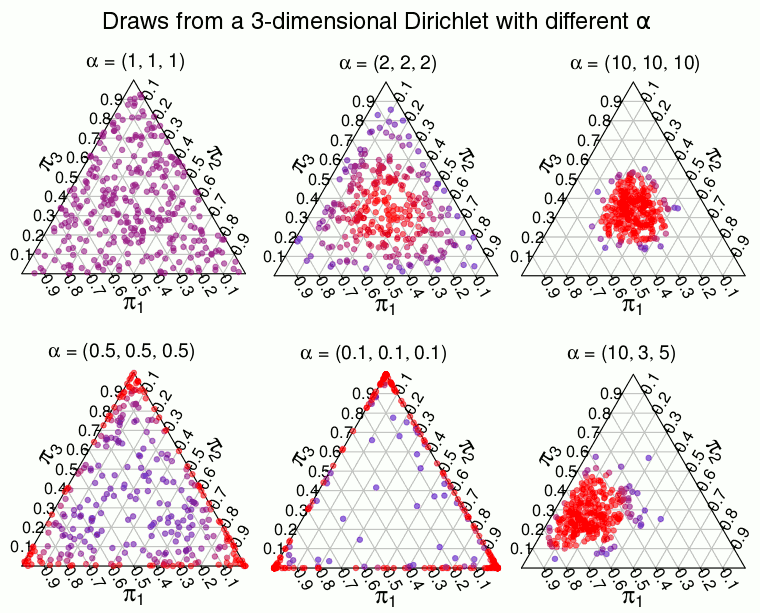
\includegraphics[scale=0.4]{dirichlet_plot.png}
    \caption{Dirichlet Distribution Examples}
    \label{}
\end{figure}

Now let's use Dirichlet distribution with parameters $\vec{\alpha}=(\alpha_1,...,\alpha_J)$ to estimate $\mathbb{E}[\vec{\theta}\mid \vec{Z}]$.

As $f(\vec{Z}\mid\vec{\theta})=\prod_{j=1}^J\theta_j^{N_j}$, we can compute the posterior beliefs
\begin{equation}
    \begin{aligned}
        \pi(\vec{\theta}\mid \vec{Z})&=\frac{f(\vec{Z}\mid \vec{\theta})P(\vec{\theta})}{\int f(\vec{Z}\mid \vec{\theta}')P(\vec{\theta}')d\vec{\theta}'}=\frac{\Gamma(\sum_{j=1}^J (N_j+\alpha_j))}{\sum_{j=1}^N\Gamma(N_j+\alpha_j)}\prod_{j=1}^J\theta_j^{N_j+\alpha_j-1}
    \end{aligned}
    \nonumber
\end{equation}
That is
\begin{equation}
    \begin{aligned}
        \theta\mid\vec{Z}\sim \text{Dirichlet}(\bar{\alpha}), \text{ where }\bar{\alpha}_j=\alpha_j+N_j, \forall j
    \end{aligned}
    \nonumber
\end{equation}
\subsubsection*{Simulate samples from Dirichlet distribution}
\begin{definition}[Simulate samples from $\text{Dirichlet}(\vec{\alpha})$]
    \normalfont
    \begin{enumerate}[1.]
        \item Consider a series of independent Gamma random variable $w_i\sim \text{Gamma}(\alpha_i,1), i=1,...,J$;
        \item Define $v_i=\frac{w_i}{\sum_{j=1}^J w_j}$;
        \item We have $(v_1,...,v_J)\sim \text{Dirichlet}(\alpha_1,...,\alpha_J)$.
    \end{enumerate}
\end{definition}

\subsection{Haldane Prior}
We may also begin with an uninformative prior, an improper prior, $\text{Dirichlet}(\vec{\alpha})$, where $\vec{\alpha} \rightarrow 0$. $\pi(\theta)\varpropto \frac{1}{\theta_1\theta_2\cdots\theta_J}$.

Under this prior, the posterior is $\text{Dirichlet}(N_1,...,N_J)$, where $N_j=\sum_{i=1}^N \mathbf{1}\{Z_i=z_j\}$.

\subsection{Linear Model Case}
Each sample is $Z_i=(1,X_{1,i},X_{2,i},X_{3,i},X_{4,i})$. The linear regression coefficient is $\beta=\mathbb{E}[XX']^{-1}\mathbb{E}[XY]$, and $\mathbb{E}^*[Y\mid X=x]=x'\beta$.

\subsection{Bernoulli Case}
Consider the problem of Example \ref{ex:square_loss}. Given $N$ random sample $\{Z_1,...,Z_N\}$ from a Bernoulli distribution with parameter $\theta$ and the sum $\sum_{i=1}^N Z_i=S$.

Consider a series of Gamma random variable $w_i^{(t)}\sim \text{Gamma}(1,1)$ from time $t=1,...,T$. Then, we have
\begin{equation}
    \begin{aligned}
        \sum_{i=1}^N w_i^{(t)} \mathbf{1}_{\{Z_i=1\}}&\sim \text{Gamma}(S,1)\\
        \sum_{i=1}^N w_i^{(t)} \mathbf{1}_{\{Z_i=0\}}&\sim \text{Gamma}(N-S,1)
    \end{aligned}
    \nonumber
\end{equation}
Define $v_i^{(t)}=\frac{w_i^{(t)}}{\sum_{j=1}^N w_j^{(t)}}$. Based on the property of Gamma distribution, we have $\mathbb{E}[w_i^{(t)}]=\text{Var}[w_i^{(t)}]=1$ and $\mathbb{E}[v_i^{(t)}]=\frac{1}{N}$.

As the relation between Gamma distribution and Beta distribution, we have
\begin{equation}
    \begin{aligned}
        \frac{\text{Gamma}(S,1)}{\text{Gamma}(S,1)+\text{Gamma}(N-S,1)}\sim \text{Beta}(S,N-S)
    \end{aligned}
    \nonumber
\end{equation}
Hence, we can define
\begin{equation}
    \begin{aligned}
        \hat{\theta}^{(t)}&=\sum_{i=1}^N v_i^{(t)}Z_i\\
        &=\sum_{i=1^N}\frac{w_i^{(t)}Z_i}{\sum_{j=1}^N w_j^{(t)}}\sim \text{Beta}(S,N-S)
    \end{aligned}
    \nonumber
\end{equation}
which is close to the posterior beliefs in Example \ref{ex:square_loss} and can be seen as the posterior beliefs drawn from an \underline{improper prior}: $\theta\sim \text{Beta}(\epsilon,\epsilon), \epsilon \rightarrow 0$, which has p.d.f. $\pi(\theta)=\frac{1}{\theta(1-\theta)}$.

We use $$\frac{1}{T}\sum_{t=1}^T\hat{\theta}^{(t)}\approx \mathbb{E}[\theta^{(t)}|\{Z_1,...,Z_n\}]$$ to estimate $\mathbb{E}[\theta^{(t)}|\{Z_1,...,Z_n\}]$.





\chapter{Linear Predictors / Regression}
\section{Best Linear Predictor}
Consider a prediction problem that the distribution $F_{X,Y}$ is known, we observe $X=\begin{pmatrix}
    1\\
    R
\end{pmatrix}\in \mathbb{R}^{K\times 1}$ and predict $Y\in \mathbb{R}$. Only linear functions of $X$ are allowed $\mathcal{L}=\{X'b:b\in \mathbb{R}^K\}$. We use square experience loss $(Y-X'b)^2$. We want to minimze Risk (mean squared error) $$\mathbb{E}_{X,Y}[(Y-X'b)^2]=\int_{x,y}(y-x'b)^2f_{x,y}(x,y)dxdy$$

\begin{assumption}
    Following inference is based on assumptions:
    \begin{enumerate}[(i).]
        \item $\mathbb{E}[Y^2]<\infty$;
        \item $\mathbb{E}[\|X\|^2]<\infty$ (Frobenius norm);
        \item $\mathbb{E}[(\alpha'X)^2]>0$ for any non-zero $\alpha\in \mathbb{R}^K$.
    \end{enumerate}
\end{assumption}

Let $\beta_0=\arg\min_{b\in \mathbb{R}^k}\mathbb{E}_{X,Y}[(Y-X'b)^2]$. By the F.O.C.
\begin{equation}
    \begin{aligned}
        \mathbb{E}[X(Y-X'\beta_0)]=0\\
        \mathbb{E}[XY]-\mathbb{E}[XX']\beta_0=0\\
        \mathbb{E}[XY]=\underbrace{\mathbb{E}[XX']}_{non-singular}\beta_0\\
        \beta_0=\mathbb{E}[XX']^{-1}\mathbb{E}[XY]
    \end{aligned}
    \nonumber
\end{equation}
\begin{proposition}[Best Linear Predictor]
    Hence, the mean-squared error minimizing linear predictor of $Y$ given $X$ is
    \begin{equation}
        \begin{aligned}
            \mathbb{E}^*[Y|X]=X'\beta_0, \text{ where }\beta_0=\mathbb{E}[XX']^{-1}\mathbb{E}[XY]
        \end{aligned}
        \nonumber
    \end{equation}
\end{proposition}
\begin{equation}
    \begin{aligned}
        \mathbb{E}_{X,Y}[X(\underbrace{Y-X'\beta_0}_{\triangleq u})]=\begin{pmatrix}
            \mathbb{E}[u]\\
            \mathbb{E}[uR]
        \end{pmatrix}=\boldsymbol{0}
    \end{aligned}
    \nonumber
\end{equation}
Hence, we have $\mathbb{E}[u]=0$, then $\mathbb{E}[uR]=0=\text{Cov}(u,R)$.
\begin{lemma}
    $\mathbb{E}[u]=\mathbb{E}[uR]=\text{Cov}(u,R)=0$, where $u=Y-\mathbb{E}^*[Y|X]$.
\end{lemma}
If $u>0$, it is underpredicting and if $u<0$, it is overpredicting.

\subsection*{Result 1 (ure Partitioned Inverse Formula)}
When we separate the constant term from other variables, we can write the \underline{Best Linear Predictor} as:
\begin{proposition}[Best Linear Predictor (ure Partitioned Inverse Formula)]
    $X=\begin{pmatrix}
        1\\
        R
    \end{pmatrix}$, $\beta_0=\begin{pmatrix}
        \alpha_0\\
        \beta_*
    \end{pmatrix}$, $\mathbb{E}[XX']^{-1}=\begin{bmatrix}
        1	& \mathbb{E}[R]'\\
        \mathbb{E}[R]	&\mathbb{E}[RR']
    \end{bmatrix}^{-1}$, $\mathbb{E}[XY]=\begin{pmatrix}
        \mathbb{E}[Y]\\
        \mathbb{E}[RY]
    \end{pmatrix}$. Then,
    \begin{equation}
        \begin{aligned}
            \alpha_0=\mathbb{E}[Y]-\mathbb{E}[R]'\beta_*\\
            \beta_*=\underbrace{\text{Var}(R)^{-1}}_{(K-1)\times(K-1)}\times \underbrace{\text{Cov}(R,Y)}_{(K-1)\times 1}
        \end{aligned}
        \nonumber
    \end{equation}
\end{proposition}

\section{Convergence of OLS}
\subsection{Approximation}
OLS Fit is
\begin{equation}
    \begin{aligned}
        \hat{\beta}=\left[\frac{1}{N}\sum_{i=1}^N X_i X'_i\right]^{-1}\left[\frac{1}{N}\sum_{i=1}^N X_iY_i\right]
    \end{aligned}
    \nonumber
\end{equation}
\begin{theorem}[Weak Law of Large Numbers (wLLN)]
    The weak law of large numbers (also called Khinchin's law) states that the sample average \underline{converges in probability} towards the expected value.
    $${\displaystyle {\begin{matrix}{}\\{\overline {X}}_{n}\ {\xrightarrow {P}}\ \mu \qquad {\text{when}}\ n\to \infty .\\{}\end{matrix}}}$$
    That is, for any positive number $\varepsilon$,
    $${\displaystyle \lim _{n\to \infty }\Pr \!\left(\,|{\overline {X}}_{n}-\mu |<\varepsilon \,\right)=1.}$$
\end{theorem}
\begin{enumerate}
    \item By LLN: $\frac{1}{N}\sum_{i=1}^N X_iY_i\xrightarrow{P} \mathbb{E}[XY]$
    \item By LLN and $f(X)=X^{-1}$ is continuous, $\left[\frac{1}{N}\sum_{i=1}^N X_iX'_i\right]\xrightarrow{P} \mathbb{E}[XX']^{-1}$
    \item Hence, $$\hat{\beta}=\left[\frac{1}{N}\sum_{i=1}^N X_i X'_i\right]^{-1}\left[\frac{1}{N}\sum_{i=1}^N X_iY_i\right] \xrightarrow{P} \mathbb{E}[XX']^{-1}\mathbb{E}[XY]= \beta_0$$
\end{enumerate}

\begin{theorem}[Central Limit Theorem (CLT)]\label{CLT}
    $$Z=\frac{\overline{X}-\mu}{\frac{\sigma}{\sqrt{n}}} \xrightarrow {D} N(0,1) \text{ when}\ n\to \infty$$
    $Z$ \underline{converges in distribution} to $N(0,1)$ as $n\to \infty$

    (converges in distribution: $P(\frac{\overline{X}-\mu}{\frac{\sigma}{\sqrt{n}}}\leq a)\rightarrow \frac{1}{\sqrt{2\pi}}\int_{-\infty}^ae^{-\frac{x^2}{2}}dx$)
\end{theorem}
Application to OLS: Let $u=Y-X'\beta_0$. Then,
\begin{equation}
    \begin{aligned}
        \hat{\beta}&=\left[\frac{1}{N}\sum_{i=1}^N X_i X'_i\right]^{-1}\left[\frac{1}{N}\sum_{i=1}^N X_iY_i\right]\\
        &=\left[\frac{1}{N}\sum_{i=1}^N X_i X'_i\right]^{-1}\left[\frac{1}{N}\sum_{i=1}^N X_i(u_i+X'_i\beta_0)\right]\\
        &=\beta_0+\left[\frac{1}{N}\sum_{i=1}^N X_i X'_i\right]^{-1}\left[\frac{1}{\sqrt{N}}\sum_{i=1}^N X_i u_i\right]
    \end{aligned}
    \nonumber
\end{equation}
Then,
\begin{equation}
    \begin{aligned}
        \sqrt{N}(\hat{\beta}-\beta_0)&=\left[\frac{1}{N}\sum_{i=1}^N X_iX
        '_i\right]^{-1}\left[\frac{1}{\sqrt{N}}\sum_{i=1}^N X_i u_i\right]
    \end{aligned}
    \nonumber
\end{equation}
\begin{enumerate}
    \item By LLN, $\left[\frac{1}{N}\sum_{i=1}^N X_iX
    '_i\right]^{-1} \xrightarrow{P} \mathbb{E}[XX']^{-1}\triangleq \Gamma_0^{-1}$.
    \item By CLT, $\left[\frac{1}{\sqrt{N}}\sum_{i=1}^N X_i u_i\right]\sim \mathcal{N}(0,\Omega_0)$, where
    \begin{equation}
        \begin{aligned}
            \Omega_0=Var[X_iu_i]=\mathbb{E}[\|X_iu_i\|^2]=\mathbb{E}[\|x_i\|^2u_i^2]\leq \left(\mathbb{E}[\|x_i\|^4]\right)^\frac{1}{2}\mathbb{E}[u_i^4]^{\frac{1}{2}}
        \end{aligned}
        \nonumber
    \end{equation}
    Hence,
    \begin{equation}
        \begin{aligned}
            \sqrt{N}(\hat{\beta}-\beta_0) \xrightarrow{D} N\left(0,\Gamma_0^{-1}\Omega_0 \Gamma_0^{-1}\right)
        \end{aligned}
        \nonumber
    \end{equation}
\end{enumerate}
The estimation of $\Gamma_0$ and $\Omega_0$:
\begin{equation}
    \begin{aligned}
        \hat{\Gamma}&=\frac{1}{N}\sum_{i=1}^N X_i X'_i\\
        \hat{\Omega}&=\frac{1}{N}\sum_{i=1}^N X_i\hat{u_i}\hat{u_i}'X'_i,\quad \text{where }\hat{u_i}=Y_i-X'_i\hat{\beta}
    \end{aligned}
    \nonumber
\end{equation}
We have
\begin{equation}
    \begin{aligned}
        \hat{\Gamma}^{-1}\hat{\Omega}\hat{\Gamma}^{-1}\xrightarrow{P} \Gamma_0^{-1}\Omega_0 \Gamma_0^{-1}
    \end{aligned}
    \nonumber
\end{equation}
Then,
\begin{equation}
    \begin{aligned}
        \hat{\beta}\xrightarrow{approx}N\left(\beta_0,\frac{\hat{\Gamma}^{-1}\hat{\Omega}\hat{\Gamma}^{-1}}{N}\right)
    \end{aligned}
    \nonumber
\end{equation}

\subsection{Testing and Confidence Interval}
Let $\hat{\Lambda}=\hat{\Gamma}^{-1}\hat{\Omega}\hat{\Gamma}^{-1}$, $\Lambda=\Gamma_0^{-1}\Omega_0 \Gamma_0^{-1}$, $\sqrt{N}(\hat{\beta}_k-\beta_k) \xrightarrow{D} N\left(0,\Lambda_{kk}\right)$. Hence,
\begin{equation}
    \begin{aligned}
        T_N\triangleq \sqrt{N}\Lambda_{kk}^{-\frac{1}{2}}\left(\hat{\beta}_k-\beta_k\right)\xrightarrow{D} N(0,1)
    \end{aligned}
    \nonumber
\end{equation}

Consider the event $A=\mathbf{1}\left\{|T_N|\leq 1.96\right\}$. We have
\begin{equation}
    \begin{aligned}
        \textnormal{Pr}(A=1)=\Phi(1.96)-\Phi(-1.96)=0.95
    \end{aligned}
    \nonumber
\end{equation}
Specifically,
\begin{equation}
    \begin{aligned}
        A&=\mathbf{1}\left\{|T_N|\leq 1.96\right\}\\
        &=\mathbf{1}\left\{\hat{\beta}_k-1.96\frac{\Lambda_{kk}^{\frac{1}{2}}}{\sqrt{N}}\leq\beta_k\leq \hat{\beta}_k+1.96\frac{\Lambda_{kk}^{\frac{1}{2}}}{\sqrt{N}}\right\}
    \end{aligned}
    \nonumber
\end{equation}
The ``Random Interval'' is
\begin{equation}
    \begin{aligned}
        \left[\hat{\beta}_k-1.96\frac{\Lambda_{kk}^{\frac{1}{2}}}{\sqrt{N}}, \hat{\beta}_k+1.96\frac{\Lambda_{kk}^{\frac{1}{2}}}{\sqrt{N}}\right]
    \end{aligned}
    \nonumber
\end{equation}


\subsection*{Testing Linear Restrictions}
Let $\theta=H\beta$, where $H$ is $p\times k$ and $\beta$ is $k\times 1$.
\begin{equation}
    \begin{aligned}
        H_0: \theta=\theta_0;\quad H_1:\theta\neq \theta_0
    \end{aligned}
    \nonumber
\end{equation}
We have
\begin{equation}
    \begin{aligned}
        \sqrt{N}(\hat{\theta}-\theta_0)=H\sqrt{N}\left(\hat{\beta}-\beta_0\right)\xrightarrow[H_0]{D} N(0,H\Lambda_0 H')
    \end{aligned}
    \nonumber
\end{equation}
Moreover,
\begin{equation}
    \begin{aligned}
        W_0=N\left(\hat{\theta}-\theta_0\right)(H\Lambda_0 H')^{-1}\left(\hat{\theta}-\theta_0\right)\xrightarrow[H_0]{D}\chi_p^2
    \end{aligned}
    \nonumber
\end{equation}
where $\mathbb{E}[\chi_p^2]=p$.


\section{Long, Short, Auxilary Regression}
$Y\in \mathbb{R}^{1}$, $X\in \mathbb{R}^{K}$, $K\in \mathbb{R}^{J}$.
Consider a researcher interested in the conditional distribution of the logarithm of weekly wages ($Y\in \mathbb{R}^{1}$) given years of competed schooling ($X\in \mathbb{R}^{K}$) and vector of additional worker attributes. This vector could include variables such as age, childhood test scores, and race. Let $W$ be this $J \times 1$ vector of additional variables.

We can run regression by two ways:
\begin{enumerate}
    \item Long regression: $\mathbb{E}^*[Y|X,W]=X'\beta_0+W'\gamma_0$.
    \item Short regression: $\mathbb{E}^*[Y|X]=X'b_0$.
\end{enumerate}
\begin{proposition}[Long Regression]
    Long regression is another form of best linear predictor.
    \begin{equation}
        \begin{aligned}
            \mathbb{E}^*[Y|X,W]&=\mathbb{E}^*[Y|Z]\\
            &=Z'\left(\mathbb{E}[ZZ']^{-1}\mathbb{E}[ZY]\right)\\
            &=X'\beta_0+W'\gamma_0
        \end{aligned}
        \nonumber
    \end{equation}
    where $\begin{pmatrix}
        \beta_0\\
        \gamma_0
    \end{pmatrix}=\mathbb{E}[ZZ']^{-1}\mathbb{E}[ZY]$, $Z=\begin{pmatrix}
        X\\
        W
    \end{pmatrix}$.
\end{proposition}

\begin{proposition}[Auxiliary Regression]
    $$\mathbb{E}^*[W|X]=\Pi_0 X$$
    which is multivariate regression. For each row $j=1,...,J$, $$\mathbb{E}^*[W_j|X]=X'\Pi_{j0}$$
    where $\Pi_{j0}=\mathbb{E}[XX']^{-1}\mathbb{E}[XW_j]$ and $\Pi_0=\begin{pmatrix}
        \Pi_{10}'\\
        \vdots\\
        \Pi_{J0}'
    \end{pmatrix}=\mathbb{E}[WX']\mathbb{E}[XX']^{-1}$.
\end{proposition}
\begin{theorem}[Law of Iterated Linear Predictors (LILP)]
    $$\mathbb{E}^*[Y|X]=\mathbb{E}^*[\mathbb{E}^*[Y|X,W]|X]$$
\end{theorem}
\underline{Facts:} Linear predictor is linear operator, $\mathbb{E}^*[X+Y|W]=\mathbb{E}^*[X|W]+\mathbb{E}^*[Y|W]$.\\
Let $Y=\mathbb{E}^*[Y|X,W]+u=X'\beta_0+W'\gamma_0+u$. Then,
\begin{equation}
    \begin{aligned}
        \mathbb{E}^*[Y|X]&=\mathbb{E}^*[X'\beta_0+W'\gamma_0+u|X]\\
        &=\mathbb{E}^*[X'\beta_0|X]+\mathbb{E}^*[W'\gamma_0|X]+\mathbb{E}^*[u|X]\\
        &=X'\beta_0+(\Pi_0X)'\gamma_0+0\\
        &=X'(\underbrace{\beta_0+\Pi_0'\gamma_0}_{b_0})
    \end{aligned}
    \nonumber
\end{equation}
\begin{proposition}[Short Regression]
    $$\mathbb{E}^*[Y|X]=X'b_0$$
    where $b_0=\beta_0+\Pi_0'\gamma_0$.
\end{proposition}

\section{Residual Regression}
Let the variation in $W$ unexplained by $X$.
\begin{equation}
    \begin{aligned}
        \underbrace{V}_{J\times 1}=\underbrace{W}_{J\times 1}-\underbrace{\mathbb{E}^*[W|X]}_{J\times 1}=W-\Pi_0X
    \end{aligned}
    \nonumber
\end{equation}
\begin{proposition}[Residual Regression]
    Let $\tilde{Y}=Y-\mathbb{E}^*[Y|X]$,
    $$\mathbb{E}^*[\tilde{Y}|V]=V'\gamma_0$$
\end{proposition}
\begin{proof}
    \begin{equation}
        \begin{aligned}
            Y&=X'\beta_0+W'\gamma_0+u\\
            \tilde{Y}&=X'\beta_0-\mathbb{E}^*[Y|X]+W'\gamma_0+u\\
            &=-X'(\Pi'_0\gamma_0)+W'\gamma_0+u\\
            &=V'\gamma_0+u\\
            \mathbb{E}^*[\tilde{Y}|V]&=V'\gamma_0
        \end{aligned}
        \nonumber
    \end{equation}
\end{proof}
By long regression,
\begin{equation}
    \begin{aligned}
        \mathbb{E}^*[Y|X,W]&=X'\beta_0+W'\gamma_0\\
        &=X'b_0-X'(\Pi'_0\gamma_0)+W'\gamma_0\\
        &=X'b_0+V'\gamma_0\\
        &=\mathbb{E}^*[Y|X]+\mathbb{E}^*[\tilde{Y}|V]
    \end{aligned}
    \nonumber
\end{equation}

\begin{theorem}[Frisch-Waugh Theorem]
    \begin{equation}
        \begin{aligned}
            \mathbb{E}^*[Y|X,V]&=\mathbb{E}^*[Y|X]+\mathbb{E}^*[Y|V]-\mathbb{E}[Y]\\
            &=\mathbb{E}^*[Y|X,W]
        \end{aligned}
        \nonumber
    \end{equation}
\end{theorem}


\begin{lemma}
    If $Cov(X,W)=0$, then
    \begin{equation}
        \begin{aligned}
            \mathbb{E}^*[Y|X,W]=\mathbb{E}^*[Y|X]+\mathbb{E}^*[Y|W]-\mathbb{E}[Y]
        \end{aligned}
        \nonumber
    \end{equation}
\end{lemma}
\begin{proof}
    Let $u=Y-\mathbb{E}^*[Y|X,W]$.
    \begin{equation}
        \begin{aligned}
            0&=\mathbb{E}[uW]\\
            &=\mathbb{E}[(Y-\mathbb{E}^*[Y|X]-\mathbb{E}^*[Y|W]+\mathbb{E}[Y])W]\\
            &=\underbrace{\mathbb{E}[(Y-\mathbb{E}^*[Y|W])W]}_{=0 \text{ by F.O.C.}}-\underbrace{\mathbb{E}[\mathbb{E}^*[Y|X]]}_{=\mathbb{E}[Y]}\mathbb{E}[W]+\mathbb{E}[Y]\mathbb{E}[W]
        \end{aligned}
        \nonumber
    \end{equation}
\end{proof}


\section{Card-Krueger Model}
Consider a model about log-learning based on schooling, ability, luck.
\begin{equation}
    \begin{aligned}
        Y(s)=\alpha_0+\beta_0 \underbrace{s}_{\text{schooling }s\in \mathbb{S}} +\underbrace{A}_\text{ability} + \underbrace{V}_\text{luck}
    \end{aligned}
    \nonumber
\end{equation}
Given a cost function about $s$:
\begin{equation}
    \begin{aligned}
        C(s)=\underbrace{C}_\text{cost heterogeneity}s+\frac{k_0}{2}s^2
    \end{aligned}
    \nonumber
\end{equation}
\begin{assumption}
    We assume
    \begin{enumerate}
        \item Information set $I_0=(C,A)$ are known by agent when choosing schooling.
        \item $V$ is independent of $C,A$: $V|C,A\triangleq V$.
    \end{enumerate}
\end{assumption}
Then, the observed schooling $s$ should satsify
\begin{equation}
    \begin{aligned}
        s&=\arg\max_s \mathbb{E}[Y(s)-C(s)\mid I_0]\\
        &=\arg\max_s \alpha_0+\beta_0 s+A-Cs-\frac{k_0}{2}s^2
    \end{aligned}
    \nonumber
\end{equation}
By F.O.C.
\begin{equation}
    \begin{aligned}
        \beta_0-C-k_0 s=0 \Rightarrow s=\frac{\beta_0-C}{k_0}
    \end{aligned}
    \nonumber
\end{equation}
\begin{enumerate}
    \item \textbf{Long Regression}:
    \begin{equation}
        \begin{aligned}
            \mathbb{E}^*[Y|s,A]=\alpha_0+\beta_0s+A
        \end{aligned}
        \tag{LR}
        \label{LR}
    \end{equation}
    \item Short Regression: $$\mathbb{E}^*[Y|s]=a_0+b_0s$$
    \item \textbf{Auxillary Regression}: By the best linear predictor, the $\mathbb{E}^*[A|s]$ can be written as
    \begin{equation}
        \begin{aligned}
            \mathbb{E}^*[A|s]&=\mathbb{E}[A]-\frac{\text{Cov}(A,s)}{\text{Var}(s)}\mathbb{E}[s]+\frac{\text{Cov}(A,s)}{\text{Var}(s)}s\\
            &=\mathbb{E}[A]-\eta_0\mathbb{E}[s]+\eta_0 s
        \end{aligned}
        \tag{AR}
        \label{AR}
    \end{equation}
    where $\eta_0=\frac{\text{Cov}(A,s)}{\text{Var}(s)}$ and $s=\frac{\beta_0-C}{k_0}$ and $\mathbb{E}[s]=\frac{\beta_0-\mu_C}{k_0}$,
    \begin{equation}
        \begin{aligned}
            \text{Cov}(A,s)&=\text{Cov}\left(A,\frac{\beta_0-C}{k_0}\right)=-\frac{\text{Cov}(A,C)}{k_0}=-\frac{\sigma_{AC}}{k_0}\\
            \text{Var}(s)&=\text{Var}\left(\frac{\beta_0-C}{k_0}\right)=\frac{\sigma_C^2}{k_0^2}\\
            \eta_0&=-k_0\frac{\sigma_{AC}}{\sigma_C^2}=-k_0\frac{\sigma_{AC}}{\sigma_A\sigma_C}\frac{\sigma_A}{\sigma_C}=-k_0\rho_{AC}\frac{\sigma_A}{\sigma_C}
        \end{aligned}
        \nonumber
    \end{equation}
    The Auxillary Regression is written as
    \begin{equation}
        \begin{aligned}
            \mathbb{E}^*[A|s]=\mathbb{E}[A]+k_0\rho_{AC}\frac{\sigma_A}{\sigma_C}\frac{\beta_0-\mu_C}{k_0}-k_0\rho_{AC}\frac{\sigma_A}{\sigma_C} s\\
            =\mathbb{E}[A]+\rho_{AC}\frac{\sigma_A}{\sigma_C}(\beta_0-\mu_C)-k_0\rho_{AC}\frac{\sigma_A}{\sigma_C} s
        \end{aligned}
        \tag{AR-1}
        \label{AR-1}
    \end{equation}
    Hence, the \textbf{Short Regression}
    \begin{equation}
        \begin{aligned}
            \mathbb{E}^*[Y|s]&=\mathbb{E}^*\left[\mathbb{E}^*[Y|s,A]|s\right]\\
            &=\mathbb{E}^*\left[\alpha_0+\beta_0s+A|s\right]\\
            &=\alpha_0+\beta_0s+\mathbb{E}^*[A|s]\\
            &=\underbrace{\alpha_0+\mathbb{E}[A]+\rho_{AC}\frac{\sigma_A}{\sigma_C}(\beta_0-\mu_C)}_{a_0}+\underbrace{\left(\beta_0-k_0\rho_{AC}\frac{\sigma_A}{\sigma_C}\right)}_{b_0}s
        \end{aligned}
        \tag{SR}
        \label{SR}
    \end{equation}
\end{enumerate}

\subsection{Proxy Variable Regression}
What if we don't observe $A$ or $C$. We observe some observed variables $W$ (\textbf{proxy variable}) instead.
\begin{assumption}
    We assume
    \begin{enumerate}
        \item Redundancy: $\mathbb{E}^*[Y|s,A,W]=\mathbb{E}^*[Y|s,A]$ ($W$ doesn't give extra information).
        \item Conditional Uncorrelatedness: $\mathbb{E}^*[A|s,W]=\mathbb{E}^*[A|W]=\Pi_0+W'\Pi_W$ (Auxillary Regression).
        \item Conditional Independence: $C\perp A | W=w$.
    \end{enumerate}
\end{assumption}
The \textbf{Proxy Variable Regression} is given by
\begin{equation}
    \begin{aligned}
        \mathbb{E}^*[Y|s,W]&=\mathbb{E}^*\left[\mathbb{E}^*[Y|s,A,W]|s,W\right]\\
        &=\mathbb{E}^*\left[\mathbb{E}^*[Y|s,A]|s,W\right]\\
        &=\mathbb{E}^*[\alpha_0+\beta_0s+A|s,W]\\
        &=\alpha_0+\beta_0s+(\Pi_0+W'\Pi_W)\\
        &=(\alpha_0+\Pi_0)+\beta_0 s+ W'\Pi_W
    \end{aligned}
    \tag{PVR}
    \label{PVR}
\end{equation}
A \underline{general form} of \textbf{Proxy Variable Regression} with
\begin{enumerate}
    \item Long Regression: $\mathbb{E}^*[Y|X,A]=X'\beta_0+A'\gamma_0$
    \item Redundancy: $\mathbb{E}^*[Y|X,A,W]=\mathbb{E}^*[Y|X,A]$
    \item Conditional Uncorrelatedness: $\mathbb{E}^*[A|X,W]=\mathbb{E}^*[A|W]=\Pi_0 W$\\
    where $\Pi_0$ is $P\times J$, $W$ is $J\times 1$, and $A$ is $P\times 1$.
\end{enumerate}
\begin{equation}
    \begin{aligned}
        \mathbb{E}^*[Y|X,W]&=\mathbb{E}^*\left[\mathbb{E}^*[Y|X,A,W]|X,W\right]\\
        &=\mathbb{E}^*\left[\mathbb{E}^*[Y|X,A]|X,W\right]\\
        &=\mathbb{E}^*\left[X'\beta_0+A'\gamma_0|X,W\right]\\
        &=X'\beta_0+\mathbb{E}^*[A|X,W]'\gamma_0\\
        &=X'\beta_0+W'\Pi'_0\gamma_0
    \end{aligned}
    \nonumber
\end{equation}

\section{Instrumental Variables}
\subsection{Motivation}
Suppose we want to estimate an OLS model $y=\beta^Tx+e$, where $x\in \mathbb{R}^k$. The OLS estimator is given by
\begin{equation}
    \begin{aligned}
        \hat{\beta}_\text{OLS}=\left(\frac{1}{m}\sum_{i=1}^mX_iX_i^T\right)^{-1}\left(\frac{1}{m}\sum_{i=1}^mX_iY_i\right)
    \end{aligned}
    \nonumber
\end{equation}
which converges (in probability) to
\begin{equation}
    \begin{aligned}
        \mathbb{E}_{P_0}[XX^T]^{-1}\mathbb{E}_{P_0}[XY]=\beta+\mathbb{E}_{P_0}[XX^T]^{-1}\underbrace{\mathbb{E}_{P_0}[Xe]}_\text{assumed to be $0$ (Exogeneity)}
    \end{aligned}
    \nonumber
\end{equation}
What if the exogeneity doesn't hold?

\begin{example}
    \begin{enumerate}
        \item $y=\beta x^*+e$, where $\mathbb{E}[x^*e]=0$. However, we don't have $x^*$ and we only have a noisy variable $x=x^*+v$ (with $\mathbb{E}[v]=0$). Then, $y=\beta(x-v)+e=\beta x+\epsilon$, where $\epsilon:=e-\beta v$. The probability limits of the OLS estimator satisfies
        \begin{equation}
            \begin{aligned}
                \hat{\beta}_\text{OLS}-\beta=\frac{\mathbb{E}_{P_0}[x\epsilon]}{\mathbb{E}_{P_0}[x^2]}=\frac{\mathbb{E}_{P_0}[(x^*+v)(e-\beta v)]}{\mathbb{E}_{P_0}[(x^*+v)^2]}=-\frac{\beta\mathbb{E}_{P_0}[v^2]}{\mathbb{E}_{P_0}[(x^*+v)^2]}
            \end{aligned}
            \nonumber
        \end{equation}
        Hence, it is impossible to let the estimator converge to the true $\beta$.
        \item Returns to Schooling: Consider a model $$\ln\text{Wage}=\beta_0+\beta_1\text{EDUC}+e$$
        Suppose the $e$ is correlated to both the wage and the education. Given $e$ is positively correlated to the education, the OLS estimator is over-estimating.
    \end{enumerate}
\end{example}

\subsection{I.V. Model}
Consider a model $Y=X^T\beta+e$, where $X\in \mathbb{R}^k$ and $\mathbb{E}_{P_0}[xe]\neq 0$.

\begin{definition}[Instrumental Variable]
    \normalfont
    A variable $Z\in \mathbb{R}^l$ is an \textbf{instrumental variable} if it satisfies
    \begin{enumerate}[(1).]
        \item $\mathbb{E}_{P_0}[Ze]=0$ (exogeneity).
        \item $\mathbb{E}_{P_0}[ZZ^T]$ is non-singular (tech).
        \item $\text{Rank}(\mathbb{E}_{P_0}(ZX^T))=k$ (relevance), which requires $l\geq k$.
    \end{enumerate}
\end{definition}
\begin{remark}
    Exogeneity implies ``exclusion restriction'', which means the $Z$ can't directly affect $Y$ without affecting $X$.
\end{remark}

\paragraph*{Implementation:}
\begin{enumerate}[$\circ$]
    \item Outcome Equation: $$Y=X^T\beta+e$$
    \item $1^{st}$ Stage Equation (no economic meaning, just for mathematical use): $$X=\Gamma^TZ+u$$
    where $X$ and $u$ are $k\times 1$, $\Gamma$ are $l\times k$, and $Z$ is $l\times 1$. $Z\perp u$ and $\Gamma=\mathbb{E}[ZZ^T]^{-1}\mathbb{E}[ZX^T]$.
    \item Reduced Form Equation:
    \begin{equation}
        \begin{aligned}
            Y&=\beta^TX+e\\
            &=\beta^T(\Gamma^TZ+u)+e\\
            &=\lambda^T Z+v
        \end{aligned}
        \nonumber
    \end{equation}
    where $\lambda=\Gamma\beta$ and $v=\beta^Tu+e$.\\
    Note that $\mathbb{E}[Zv]=0$, which satisfies exogeneity. Hence, we can use OLS to estimate $\lambda$.
\end{enumerate}


\paragraph*{Identification:} Suppose $\lambda$ and $\Gamma$ are known, we want to recover $\beta$.
\begin{equation}
    \begin{aligned}
        \lambda=\Gamma\beta
    \end{aligned}
    \nonumber
\end{equation}
\begin{enumerate}
    \item \underline{Case 1}: $l=k$,
    \begin{equation}
        \begin{aligned}
            \beta=\Gamma^{-1}\lambda
        \end{aligned}
        \nonumber
    \end{equation}
    where $\Gamma^{-1}$ exists by relevance.
    \item \underline{Case 2}: $l>k$,
    \begin{equation}
        \begin{aligned}
            \Gamma^T\lambda=(\Gamma^T\Gamma)\beta \Rightarrow \beta=(\Gamma^T\Gamma)^{-1}\Gamma^T\lambda
        \end{aligned}
        \nonumber
    \end{equation}
\end{enumerate}

\paragraph*{Estimation of $\Gamma$ and $\lambda$:}
\begin{enumerate}[(A).]
    \item ``Plug In''
    \begin{enumerate}
        \item The estimation of $\Gamma$ is given by
        \begin{equation}
            \begin{aligned}
                \hat{\Gamma}=\left(\frac{1}{m}\sum_{i=1}^m Z_iZ_i^T\right)^{-1}\left(\frac{1}{m}\sum_{i=1}^m Z_i X_i^T\right)
            \end{aligned}
            \tag{hG}
        \end{equation}
        The OLS estimator of regressing $X$ on $Z$ should converge to $\Gamma$ in probability.
        \item The estimation of $\lambda$ is given by
        \begin{equation}
            \begin{aligned}
                \hat{\lambda}=\left(\frac{1}{m}\sum_{i=1}^m Z_iZ_i^T\right)^{-1}\left(\frac{1}{m}\sum_{i=1}^m Z_i Y_i\right)
            \end{aligned}
            \nonumber
            \label{hG}
        \end{equation}
        which converges to $\lambda$ in probability.
    \end{enumerate}
    \item ``2SLS''\\
    The reduced form can also be written as
    \begin{equation}
        \begin{aligned}
            Y&=\beta^TX+e\\
            &=\beta^T(\Gamma^TZ+u)+e\\
            &=\beta^T\underbrace{(\Gamma^TZ)}_{W} +v
        \end{aligned}
        \tag{hl}
        \label{hl}
    \end{equation}
    Assuming $\Gamma$ is known, we can regress $Y$ on $W$:
    \begin{equation}
        \begin{aligned}
            \tilde{\beta}&=\left(\frac{1}{m}\sum_{i=1}^m W_iW_i^T\right)^{-1}\left(\frac{1}{m}\sum_{i=1}^m W_i Y_i\right)\\
            &=\left(\Gamma^T\left(\frac{1}{m}\sum_{i=1}^m Z_iZ_i^T\right)\Gamma\right)^{-1}\Gamma^T\left(\frac{1}{m}\sum_{i=1}^m Z_i Y_i\right)
        \end{aligned}
        \nonumber
    \end{equation}
    Hence, we can estimate $\beta$ based on
    \begin{equation}
        \begin{aligned}
            \hat{\beta}_\textnormal{2SLS}=\left(\hat{\Gamma}^T\left(\frac{1}{m}\sum_{i=1}^m Z_iZ_i^T\right)\hat{\Gamma}\right)^{-1}\hat{\Gamma}^T\left(\frac{1}{m}\sum_{i=1}^m Z_i Y_i\right)
        \end{aligned}
        \nonumber
    \end{equation}
    where $\hat{\Gamma}$ is given by \eqref{hG}. Specifically, in the case of $l=k$, $\hat{\beta}_\textnormal{2SLS}=\left(\frac{1}{m}\sum_{i=1}^m Z_iX_i^T\right)^{-1}\left(\frac{1}{m}\sum_{i=1}^m Z_i Y_i\right)$.
    \begin{remark}
        Why not use the following steps?
        \begin{enumerate}
            \item Regress $X$ on $Z$ to construct $\hat{W}:=\hat{\Gamma}^TZ$.
            \item Regress $Y$ on $\hat{W}$.
        \end{enumerate}
        \textcolor{orange}{(Note that the mathematical foundation of OLS doesn't hold here because $\hat{W}$ is not i.i.d.)}
    \end{remark}
\end{enumerate}

\subsection{Weak I.V.}
The ``relevance'' of the IV doesn't hold: $\mathbb{E}[ZX^T]\approx 0$. \underline{Why this is a problem?}

Let's begin with a simple case that $l=k=1$. The 2SLS estimator is given by
\begin{equation}
    \begin{aligned}
        \hat{\beta}_\textnormal{2SLS}=\frac{\frac{1}{m}\sum_{i=1}^mZ_iY_i}{\frac{1}{m}\sum_{i=1}^mZ_iX_i}=\beta+\frac{\frac{1}{m}\sum_{i=1}^mZ_ie_i}{\frac{1}{m}\sum_{i=1}^mZ_iX_i}
    \end{aligned}
    \nonumber
\end{equation}
where the small $Z_iX_i$ may lead to a large bias.

Consider the $\mathbb{E}[ZX]=\frac{c}{\sqrt{m}},c\neq 0$. Then, the 2SLS estimator can be written as
\begin{equation}
    \begin{aligned}
        \hat{\beta}_\textnormal{2SLS}=\beta+\frac{\frac{1}{m}\sum_{i=1}^mZ_ie_i}{\frac{c}{\sqrt{m}}\frac{1}{m}\sum_{i=1}^mZ_i^2+\frac{1}{m}\sum_{i=1}^mZ_iv_i}=\beta+\frac{\frac{1}{\sqrt{m}}\sum_{i=1}^mZ_ie_i}{c\frac{1}{m}\sum_{i=1}^mZ_i^2+\frac{1}{\sqrt{m}}\sum_{i=1}^mZ_iu_i}
    \end{aligned}
    \nonumber
\end{equation}
where the $\lim_{m \rightarrow \infty}\frac{1}{\sqrt{m}}\sum_{i=1}^mZ_ie_i\sim \mathcal{N}(0,\sigma^2)$ and $\lim_{m \rightarrow \infty}\frac{1}{\sqrt{m}}\sum_{i=1}^mZ_iu_i\sim \mathcal{N}(0,r^2)$ by LLN, and $\frac{1}{m}\sum_{i=1}^mZ_i^2 \rightarrow 1+0_P(1)$ with normalized $Z$. Hence, As $m \rightarrow \infty$,
\begin{equation}
    \begin{aligned}
        \hat{\beta}_\textnormal{2SLS}\approx \beta+\frac{\mathcal{N}(0,\sigma^S)}{\mathcal{N}(c,r^2)}
    \end{aligned}
    \nonumber
\end{equation}
which gives that $\hat{\beta}_\textnormal{2SLS}$ is not good for nonzero $\mathbb{E}[ZX]$.


\section{Linear Generalized Method of Moments (Linear GMM)}
\subsection{Generalized Method of Moments (GMM)}
\begin{assumption}
    GMM model assumes that, given the true probability of data $P_0$, there exists a unique parameter $\beta$ such that
    \begin{equation}
        \begin{aligned}
            \mathbb{E}_{P_0}[g(\textnormal{Data},\beta_0)]=0
        \end{aligned}
        \nonumber
    \end{equation}
    where $g(\cdot)$ is a residual function.
\end{assumption}
$\beta_0$ is given by
\begin{equation}
    \begin{aligned}
        \beta_0=\argmin_{\beta}J(\beta,P_0)
    \end{aligned}
    \nonumber
\end{equation}
where
\begin{equation}
    \begin{aligned}
        J(\beta,P_0):=\left(\mathbb{E}_{P_0}[g(Y,X,Z,\beta)]\right)^TW\left(\mathbb{E}_{P_0}[g(Y,X,Z,\beta)]\right)
    \end{aligned}
    \nonumber
\end{equation}
and the weight matrix $W\succ 0$ (is positive definite and symmetric).

The GMM estimator is given by
\begin{equation}
    \begin{aligned}
        \hat{\beta}_\textnormal{GMM}=\argmin_{\beta}J(\beta,P_m)
    \end{aligned}
    \nonumber
\end{equation}

Using this for
\begin{enumerate}
    \item \underline{Linear Regression:} $g(Y,X,\beta):=(Y-X^T\beta)X$;
    \item \underline{IV Model:} $g(Y,X,Z,\beta)=Z(Y-X^T\beta)$, which is called Linear GMM.
\end{enumerate}

\subsection{Linear GMM}
\begin{definition}[Linear GMM]
    \normalfont
    A \textbf{Linear GMM} is defined as
    \begin{equation}
        \begin{aligned}
            \mathbb{E}_{P_0}[\underbrace{Z}_{l\times 1}(\underbrace{Y}_{1\times 1}-\beta_0^T\underbrace{X}_{k\times 1})]=0
        \end{aligned}
        \nonumber
    \end{equation}
\end{definition}

If $\textnormal{Rank}\left(\mathbb{E}_{P_0}[ZX^T]\right)=k$, there is a unique $\beta_0=$ minimizes $J(\beta,P_0)$ with $$J(\beta,P_0):=\left(\mathbb{E}_{P_0}[Z(Y-X^T\beta)]\right)^TW\left(\mathbb{E}_{P_0}[Z(Y-X^T\beta)]\right)$$
\begin{equation}
    \begin{aligned}
        J(\hat{\beta},P_0):=\left(\frac{1}{m}\sum_{i=1}^mZ_i(Y_i-X_i^T\beta)\right)^TW\left(\frac{1}{m}\sum_{i=1}^mZ_i(Y_i-X_i^T\beta)\right)
    \end{aligned}
    \nonumber
\end{equation}

The GMM estimator is given by
\begin{equation}
    \begin{aligned}
        \hat{\beta}_\textnormal{GMM}
        =\argmin_{\beta}\left(\frac{1}{m}\sum_{i=1}^mZ_i(Y_i-X_i^T\beta)\right)^TW\left(\frac{1}{m}\sum_{i=1}^mZ_i(Y_i-X_i^T\beta)\right)
    \end{aligned}
    \label{GMM_est}
\end{equation}

\begin{remark}
    $W$ matters for $\hat{\beta}_\textnormal{GMM}$.
\end{remark}
The FOC of \eqref{GMM_est} is given by
\begin{equation}
    \begin{aligned}
        \left(\frac{1}{m}\sum_{i=1}^mZ_iX_i^T\right)^TW\left(\frac{1}{m}\sum_{i=1}^mZ_iY_i-(\frac{1}{m}\sum_{i=1}^mZ_iX_i^T)\hat{\beta}_\textnormal{GMM}\right)=0
    \end{aligned}
    \nonumber
\end{equation}
Let $\hat{Q}:=\frac{1}{m}\sum_{i=1}^mZ_iX_i^T\in \mathbb{R}
^{l\times k}$. Then,
\begin{equation}
    \begin{aligned}
        \hat{\beta}_\textnormal{GMM}=\left(\hat{Q}^TW\hat{Q}\right)^{-1}\hat{Q}^TW\frac{1}{m}\sum_{i=1}^mZ_iY_i
    \end{aligned}
    \nonumber
\end{equation}
\begin{lemma}
    If $W=(\frac{1}{m}\sum_{i=1}^mZ_iZ_i^T)^{-1}$, then $\hat{\beta}_\textnormal{GMM}=\hat{\beta}_\textnormal{2SLS}$
\end{lemma}
\begin{proof}
    With $W^T=W$,
    \begin{equation}
        \begin{aligned}
            \hat{\beta}_\textnormal{GMM}&=\left(\hat{Q}^TW\hat{Q}\right)^{-1}\hat{Q}^TW\frac{1}{m}\sum_{i=1}^mZ_iY_i\\
            &\left(\hat{Q}^TWW^{-1}W\hat{Q}\right)^{-1}\hat{Q}^TW\frac{1}{m}\sum_{i=1}^mZ_iY_i\\
            &=\left((W\hat{Q})^TW^{-1}(W\hat{Q})\right)^{-1}(W\hat{Q})^T\frac{1}{m}\sum_{i=1}^mZ_iY_i\\
        \end{aligned}
        \nonumber
    \end{equation}
    Substitute $W$ by $W=(\frac{1}{m}\sum_{i=1}^mZ_iZ_i^T)^{-1}$. We have $W\hat{Q}=\hat{\Gamma}$. The lemma is proved.
\end{proof}


\subsection{Properties of Linear GMM Estimator}
\begin{theorem}[Asymptotic]
    $\sqrt{m}\left(\hat{\beta}_\textnormal{GMM}-\beta_0\right) \rightarrow \mathcal{N}(0,V_{P_0})$.
\end{theorem}
\begin{proof}
    \begin{equation}
        \begin{aligned}
            \hat{\beta}_\textnormal{GMM}&=\left(\hat{Q}^TW\hat{Q}\right)^{-1}\hat{Q}^TW\frac{1}{m}\sum_{i=1}^mZ_i\underbrace{Y_i}_{X_i^T\beta_0+e_i}\\
            &=\left(\hat{Q}^TW\hat{Q}\right)^{-1}\hat{Q}^TW\left(\underbrace{(\frac{1}{m}\sum_{i=1}^mZ_iX_i^T)}_{\hat{Q}}\beta_0+\frac{1}{m}\sum_{i=1}^mZ_ie_i\right)\\
            &=\beta_0+\left(\hat{Q}^TW\hat{Q}\right)^{-1}\hat{Q}^TW\frac{1}{m}\sum_{i=1}^mZ_ie_i
        \end{aligned}
        \nonumber
    \end{equation}
    By LLN, $\hat{Q} \stackrel{P}{\longrightarrow} Q:=\mathbb{E}[ZX^T]$. Then we have, $\hat{Q}^TW\hat{Q} \stackrel{P}{\longrightarrow} Q^TWQ$. Because $Q^TWQ$ is invertible, $(\hat{Q}^TW\hat{Q})^{-1} \stackrel{P}{\longrightarrow} (Q^TWQ)^{-1}$. So, $(\hat{Q}^TW\hat{Q})^{-1}=(Q^TWQ)^{-1}+o_{P_0}(1)$. Hence,
    \begin{equation}
        \begin{aligned}
            \hat{\beta}_\textnormal{GMM}&=\beta_0+\left((Q^TWQ)^{-1}+o_{P_0}(1)\right)(Q^TW+o_{P_0}(1))\frac{1}{m}\sum_{i=1}^mZ_ie_i\\
            &=\beta_0+((Q^TWQ)^{-1}Q^TW+o_{P_0}(1))\frac{1}{m}\sum_{i=1}^mZ_ie_i\\
            &=\beta_0+(Q^TWQ)^{-1}Q^TW\frac{1}{m}\sum_{i=1}^mZ_ie_i+o_{P_0}(1)\frac{1}{m}\sum_{i=1}^mZ_ie_i
        \end{aligned}
        \nonumber
    \end{equation}
    By orthogonality condition, $\mathbb{E}_{P_0}[Ze]=0$. And by central limit theorem, we have $\sqrt{m}\frac{1}{m}\sum_{i=1}^mZ_ie_i \rightarrow \mathcal{N}(0,\Omega_{P_0})$. Then, we represent $\hat{\beta}_\textnormal{GMM}$ as
    \begin{equation}
        \begin{aligned}
            \hat{\beta}_\textnormal{GMM}=\beta_0+(Q^TWQ)^{-1}Q^TW\frac{1}{m}\sum_{i=1}^mZ_ie_i+o_{P_0}(\frac{1}{\sqrt{m}})
        \end{aligned}
        \label{hat_beta_minus_beta}
    \end{equation}
    which is called \textbf{asymptotic linear representation}.

    Multiplying $\sqrt{m}$,
    \begin{equation}
        \begin{aligned}
            \sqrt{m}(\hat{\beta}_\textnormal{GMM}-\beta_0)&=(Q^TWQ)^{-1}Q^TW\underbrace{\frac{1}{\sqrt{m}}\sum_{i=1}^mZ_ie_i}_{\rightarrow \mathcal{N}(0,\Omega_{P_0})}+o_{P_0}(1)\\
            &\rightarrow \mathcal{N}\left(0,\underbrace{(Q^TWQ)^{-1}Q^TW\Omega_{P_0}WQ(Q^TWQ)^{-1}}_{\triangleq V_{P_0}}\right)
        \end{aligned}
        \nonumber
    \end{equation}
\end{proof}

\begin{corollary}
    $\hat{\beta}_\textnormal{GMM} \stackrel{P}{\longrightarrow} \beta_0$.
\end{corollary}
\begin{proof}
    $\hat{\beta}_\textnormal{GMM}-\beta_0=O_{P_0}(\frac{1}{\sqrt{m}}) \rightarrow o_{P_0}(1)$.
\end{proof}


\paragraph*{Efficiency Consideration} We want to choose the weight matrix to minimize the asymptotic variance within GMM estimator, $W^*=\argmin_{W}V_{P_0}$.
\begin{theorem}
    $W^*=\Omega_{P_0}^{-1}$. That is, $V^*_{P_0}:=\left(Q^T\Omega_{P_0}^{-1}Q\right)^{-1}\leq V_{P_0}, \forall W$.
\end{theorem}
Then, we want to compute the efficient GMM by $\Omega_{P_0}:=\mathbb{E}[e^2ZZ^T]$.
\begin{equation}
    \begin{aligned}
        \hat{W}^*=\left(\hat{\Omega}\right)^{-1}
    \end{aligned}
    \nonumber
\end{equation}
where $\hat{\Omega}=\frac{1}{m}\sum_{i=1}^m\hat{e}_i^2ZZ^T$ and $\hat{e}_i$ is given by
\begin{equation}
    \begin{aligned}
        \hat{e}_i:=Y_i-X_i^T\hat{\beta}
    \end{aligned}
    \nonumber
\end{equation}
where $\hat{\beta}$ can be any GMM estimator, e.g., $W=I$ or a 2SLS estimator. As long as we can make sure $\hat{\Omega}\stackrel{P}{\longrightarrow}\Omega_{P_0}$.

Finally, we have $\hat{\beta}_\textnormal{EFFI}:=\hat{W}^*=W^*+o_{P_0}(1)$,
\begin{equation}
    \begin{aligned}
        \sqrt{m}\left(\hat{\beta}_\textnormal{EFFI}-\beta_0\right) \rightarrow \mathcal{N}(0,\left(Q^T\Omega_{P_0}^{-1}Q\right)^{-1})
    \end{aligned}
    \nonumber
\end{equation}

\begin{remark}
    If $\mathbb{E}_{P_0}[e^2|Z]=\sigma^2_e$, then 2SLS is efficient.
    \begin{equation}
        \begin{aligned}
            \Omega^{-1}=\left(\mathbb{E}_{P_0}[e^2ZZ^T]\right)^{-1}=\frac{1}{\sigma^2_e}\underbrace{\left(\mathbb{E}_{P_0}[ZZ^T]\right)^{-1}}_{W\text{ used in 2SLS}}
        \end{aligned}
        \nonumber
    \end{equation}
\end{remark}


\subsection{Alternative: Continuous Updating Estimator}
Based on the idea of efficiency, we may use
\begin{equation}
    \begin{aligned}
        \hat{\beta}_\textnormal{CUE}=\argmin_{\beta}\left(\frac{1}{m}\sum_{i=1}^m g(\textnormal{Data}_i,\beta)\right)^T\left(\frac{1}{m}\sum_{i=1}^m\hat{e}_i^2ZZ^T\right)\left(\frac{1}{m}\sum_{i=1}^m g(\textnormal{Data}_i,\beta)\right)
    \end{aligned}
    \nonumber
\end{equation}
However, it may not be convex.

\subsection{Inference}
Suppose we want test $H_0:\Gamma(\beta_0)=\theta_0=0$ or $H_0: \theta_0=\Gamma(\beta_0)\neq\hat{\theta}=\Gamma(\hat{\beta})$.
\begin{theorem}[Construct Chi-square]
    By using the asymptotic variance of GMM, $V_{{P_0}}$,
    $$m(\hat{\theta}-\theta)^T\left(R(\beta_0)^TV_{P_0}R(\beta_0)\right)^{-1}(\hat{\theta}-\theta) \Rightarrow \chi^2_l$$
    where $R(\beta_0):=\frac{d \Gamma(\beta_0)}{d\beta}\in \mathbb{R}^{k\times l}$.
\end{theorem}
\begin{proof}
    Let
    $$\overbrace{m(\hat{\theta}-\theta)^T\underbrace{\left(R(\beta_0)^TV_{P_0}R(\beta_0)\right)^{-1}}_{\triangleq\Omega}(\hat{\theta}-\theta)}^\mathcal{W} \Rightarrow \chi^2_l$$
    We have
    \begin{equation}
        \begin{aligned}
            \hat{\theta}-\theta_0=\Gamma(\hat{\beta})-\Gamma(\beta_0)=\underbrace{\frac{d\Gamma(\beta_0)}{d\beta}}_{R(\beta_0)}(\hat{\beta}-\beta_0)+o_{P_0}(m^{-\frac{1}{2}})\\
            %\hat{\beta}=\beta_0+\left(Q^TWQ\right)^{-1}Q^T
        \end{aligned}
        \nonumber
    \end{equation}
    \begin{equation}
        \begin{aligned}
            \mathcal{W}=\left(\sqrt{m}R(\beta_0)(\hat{\beta}-\beta_0)+o_{P_0}(1)\right)^T\Omega \left(\sqrt{m}R(\beta_0)(\hat{\beta}-\beta_0)+o_{P_0}(1)\right)
        \end{aligned}
        \nonumber
    \end{equation}
    As $\sqrt{m}\left(\hat{\beta}-\beta_0\right)\Rightarrow \mathcal{N}(0,V_{P_0})$, by continuous mapping theorem, we have
    \begin{equation}
        \begin{aligned}
            \mathcal{W} \Rightarrow \left(\mathcal{N}(0,R(\beta_0)V_{P_0}R(\beta_0)^T)\right)^T\Omega\left(\mathcal{N}(0,R(\beta_0)V_{P_0}R(\beta_0)^T)\right)
        \end{aligned}
        \nonumber
    \end{equation}
    Let $M:=R(\beta_0)V_{P_0}R(\beta_0)^T$. Since $M$ is symmetric, it can be decomposed by $M=LL^T$. Then, $M^{-1}=(L^{T})^{-1}L^{-1}$. We have $L^{-1}M(L^{T})^{-1}=I$.\\
    Since $\Omega=M^{-1}=(L^{-1})^TL^{-1}$,
    \begin{equation}
        \begin{aligned}
            \mathcal{W}\Rightarrow \left(\mathcal{N}(0,I)\right)^T\left(\mathcal{N}(0,I)\right)=\chi^2_l
        \end{aligned}
        \nonumber
    \end{equation}
\end{proof}
Based on this theorem, we have the ``real'' Wald test for $H_0:\Gamma(\beta_0)=\theta_0=0$.
\begin{equation}
    \begin{aligned}
        \mathcal{W}=m(\hat{\theta}-\theta)^T\left(R(\hat{\beta})^T\hat{V}_{P_0}R(\hat{\beta})\right)^{-1}(\hat{\theta}-\theta) \Rightarrow \chi^2_l
    \end{aligned}
    \nonumber
\end{equation}


\subsection{OVER-ID Test}
Remind that $$J(\beta,P_0):=\left(\mathbb{E}_{P_0}[Z(Y-X^T\beta)]\right)^TW\left(\mathbb{E}_{P_0}[Z(Y-X^T\beta)]\right)$$
We want to test
$$H_0: J(\beta,P_0)=0$$
which is equivalent to $\mathbb{E}[Ze]=0$. $H_1: J(\beta,P_0)> 0$, which is equivalent to $\mathbb{E}[Ze]\neq 0$.
\begin{theorem}
    If $W$ is efficient weighting matrix ($W=\hat{\Omega}^{-1}$), then $m J(\hat{\beta},P_m) \Rightarrow \chi^2_{l-k}$
\end{theorem}
\begin{proof}
    Remind \eqref{hat_beta_minus_beta} that $\hat{\beta}=\beta_0+(Q^TWQ)^{-1}Q^TW\frac{1}{m}\sum_{i=1}^mZ_ie_i+o_{P_0}(\frac{1}{\sqrt{m}})$ and $Q:=\mathbb{E}[ZX^T]$. Then,
    \begin{equation}
        \begin{aligned}
            Z_i(Y_i-X_i^T\hat{\beta})&=Z_i(X_i^T\beta_0+e_i-X_i^T\hat{\beta})\\
            &=-Q(\hat{\beta}-\beta_0)+\frac{1}{m}\sum_{i=1}^mZ_ie_i+o_{P_0}(\frac{1}{\sqrt{m}})
        \end{aligned}
        \nonumber
    \end{equation}
    which gives
    \begin{equation}
        \begin{aligned}
            \frac{1}{m}\sum_{i=1}^mZ_i(Y_i-X_i^T\hat{\beta})=\left(I-Q(Q^TWQ)^{-1}Q^TW\right)\frac{1}{m}\sum_{i=1}^mZ_ie_i+o_{P_0}(\frac{1}{\sqrt{m}})
        \end{aligned}
        \nonumber
    \end{equation}
    By decomposing $W$ by $W:=LL^T$,
    \begin{equation}
        \begin{aligned}
            m J(\hat{\beta},P_m)=\left(L^T\frac{1}{\sqrt{m}}\sum_{i=1}^mZ_i(Y_i-X_i^T\hat{\beta})\right)^T\left(L^T\frac{1}{\sqrt{m}}\sum_{i=1}^mZ_i(Y_i-X_i^T\hat{\beta})\right)
        \end{aligned}
        \nonumber
    \end{equation}
    where
    \begin{equation}
        \begin{aligned}
            L^T\frac{1}{\sqrt{m}}\sum_{i=1}^mZ_i(Y_i-X_i^T\hat{\beta})&=\left(L^T-\underbrace{L^TQ}_{:=M}((L^TQ)^T(L^TQ))^{-1}(L^TQ)^TL^T\right)\frac{1}{\sqrt{m}}\sum_{i=1}^mZ_ie_i+o_{P_0}(1)\\
            &=\underbrace{\left(I-M(M^TM)^{-1}M^T\right)}_{:=R_M}\left(L^T\left(\frac{1}{\sqrt{m}}\sum_{i=1}^mZ_ie_i\right)\right)+o_{P_0}(1)
        \end{aligned}
        \nonumber
    \end{equation}
    where $R_M$ satisfies $R_M=R_M^TR_M$, which shows $R_M$ has eigenvalues $\in\{0,1\}$ and its number of eigenvalues equal to $1$ is $l-k$.\\
    Hence,
    \begin{equation}
        \begin{aligned}
            m J(\hat{\beta},P_m)=\left(L^T\left(\frac{1}{\sqrt{m}}\sum_{i=1}^mZ_ie_i\right)\right)^TR_M\left(L^T\left(\frac{1}{\sqrt{m}}\sum_{i=1}^mZ_ie_i\right)\right)+o_{P_0}(1)
        \end{aligned}
        \nonumber
    \end{equation}
    As $\left(L^T\left(\frac{1}{\sqrt{m}}\sum_{i=1}^mZ_ie_i\right)\right) \Rightarrow \xi \sim \mathcal{N}(0,L^T\Omega L)$. So,
    \begin{equation}
        \begin{aligned}
            mJ(\hat{\beta},P_m) \Rightarrow \xi^TR_m\xi
        \end{aligned}
        \nonumber
    \end{equation}
    If $W=\Omega^{-1}$, then $L^T\Omega L=I$, which gives
    \begin{equation}
        \begin{aligned}
            mJ(\hat{\beta},P_m) &\Rightarrow \xi_*^TR_m\xi_*,\ \xi_*\sim \mathcal{N}(0,I)\\
            &=\sum_{j=1}^{l-k}\omega_j^2,\omega_j\sim \mathcal{N}(0,1)\\
            &\sim \chi^2_{l-k}
        \end{aligned}
        \nonumber
    \end{equation}
\end{proof}
\begin{remark}
    \begin{enumerate}
        \item Test by $c_\alpha$, which gives $\textnormal{Pr}(\chi^2_{l-k}\geq c_\alpha)=\alpha\in (0,1)$.
        \item Only make sense for $l>k$.
        \begin{enumerate}
            \item You ``spent'' $k$ degrees of freedom estimating $\beta_0$.
            \item The rest $(l-k)$ is ``spent'' on testing.
        \end{enumerate}
    \end{enumerate}
\end{remark}

\subsection{Bootstrap GMM}
Now, we gives estimator by using bootstrap data,
\begin{equation}
    \begin{aligned}
        \hat{\beta}^*=\argmin_\beta J(\beta,P_m^*)
    \end{aligned}
    \nonumber
\end{equation}
where
\begin{equation}
    \begin{aligned}
        J(\beta,P_m^*):=\left(\frac{1}{m}\sum_{i=1}^mZ_i^*(Y_i^*-{X_i^*}^T\beta)-\mathbb{E}_{P_m}[Z(Y-X^T\hat{\beta})]\right)^TW\left(\frac{1}{m}\sum_{i=1}^mZ_i^*(Y_i^*-{X_i^*}^T\beta)-\mathbb{E}_{P_m}[Z(Y-X^T\hat{\beta})]\right)
    \end{aligned}
    \nonumber
\end{equation}
where $\mathbb{E}_{P_m}[Z(Y-X^T\hat{\beta})]=\frac{1}{m}\sum_{i=1}^m Z_i\hat{e}_i$, which is used to debias. Then,
\begin{equation}
    \begin{aligned}
        \hat{\beta}_\textnormal{GMM}=\left(\hat{Q}^{*T}W\hat{Q}^*\right)^{-1}\hat{Q}^{*T}W\left(\frac{1}{m}\sum_{i=1}^m(Z_i^*Y_i^*-Z_i\hat{e}_i)\right)
    \end{aligned}
    \nonumber
\end{equation}
\paragraph*{Bootstrap OVER-ID Test}
The distribution $m J(\hat{\beta}^*,P_m^*)$ is the \underline{same} as $m J(\hat{\beta},P_m)$ regardless of $W$.


\section{Panel Data Models}
\begin{definition}[Panel Data]
    \normalfont
    For each unit $i$, it has time $\{1,...,T\}$.
    \begin{center}
        \begin{tabular}{cc}
            \hline
                & $t=1$\\
                $i=1$& $\vdots$\\
                & $t=T$\\
            \hline
                & $t=1$\\
                $i=2$& $\vdots$\\
                & $t=T$\\
            \hline
            $\vdots$&$\vdots$
        \end{tabular}
    \end{center}
\end{definition}
The typical model is given by
\begin{equation}
    \begin{aligned}
        Y_{i_t}=\underbrace{\alpha_i}_\textnormal{Fixed Effect}+X_{i_t}^T\beta+\epsilon_{i_t}
    \end{aligned}
    \nonumber
\end{equation}
$\alpha_i$ is a fixed effect, which is unobserved, random, and time invariant.
\begin{assumption}
    \begin{enumerate}
        \item $\{\alpha_i,\left(X_{i_t}\right)_{t=1}^T,\left(Y_{i_t}\right)_{t=1}^T,\left(\epsilon_{i_t}\right)_{t=1}^T\}$ is i.i.d. for all $i\in\{1,...,N\}$. (Within a unit, data at different time can be dependent, which means there are no estimators within units.)
        \item $N \rightarrow \infty$, $T$ is fixed.
    \end{enumerate}
\end{assumption}

\subsection{Pooled OLS}
\begin{equation}
    \begin{aligned}
        Y_{i_t}=X_{i_t}^T\beta_0+\underbrace{e_{i_t}}_{:=\alpha_i+\epsilon_{i_t}}
    \end{aligned}
    \nonumber
\end{equation}
Use the notations of vectors $\vec{Y}_{i}:=\begin{bmatrix}
    Y_{i_1}\\
    \vdots\\
    Y_{i_T}
\end{bmatrix}$, $\vec{X}_{i}:=\begin{bmatrix}
    X_{i_1}\\
    \vdots\\
    X_{i_T}
\end{bmatrix}$, $\vec{e}_i:=\mathbf{1}\alpha_i+\vec{\epsilon}_i$, where $\mathbf{1}=\begin{bmatrix}1\\ \vdots \\ 1\end{bmatrix}$. Then, the equation can be written as
\begin{equation}
    \begin{aligned}
        \vec{Y}_i=\vec{X}_i\beta_0+\vec{e}_i
    \end{aligned}
    \nonumber
\end{equation}
The pooled OLS estimator is
\begin{equation}
    \begin{aligned}
        \hat{\beta}_\textnormal{pool}:=\left(\frac{1}{N}\sum_{i=1}^N \vec{X}_i^T \vec{X}_i\right)^{-1}\left(\frac{1}{N}\sum_{i=1}^N \vec{X}_i^T \vec{Y}_i\right)
    \end{aligned}
    \nonumber
\end{equation}
\paragraph*{Properties}
\begin{equation}
    \begin{aligned}
        \hat{\beta}_\textnormal{pool}=\beta_0+\left(\frac{1}{N}\sum_{i=1}^N \vec{X}_i^T \vec{X}_i\right)^{-1}\left(\frac{1}{N}\sum_{i=1}^N \vec{X}_i^T \vec{e}_i\right)
    \end{aligned}
    \nonumber
\end{equation}
For consistency:
\begin{enumerate}
    \item $\frac{1}{N}\sum_{i=1}^N \vec{X}_i^T \vec{X}_i \stackrel{P}{\longrightarrow} \mathbb{E}[\vec{X}^T \vec{X}]$, which is required to be non singular.
    \item $\frac{1}{N}\sum_{i=1}^N \vec{X}_i^T \vec{e}_i \stackrel{P}{\longrightarrow} \mathbb{E}[\vec{X}^T \vec{e}]$, where
    \begin{equation}
        \begin{aligned}
            \mathbb{E}[\vec{X}^T \vec{e}]=\underbrace{\mathbb{E}[\vec{X}^T \mathbf{1}\alpha]}_{\textcolor{red}{\textnormal{need assumed to be 0}}}+\underbrace{\mathbb{E}[\vec{X}^T \vec{\epsilon}]}_{:=0 \textnormal{, by assumption}}
        \end{aligned}
        \nonumber
    \end{equation}
\end{enumerate}
The pooled OLS estimator is inconsistent if $X_{it}$ is correlated with $\alpha_i$.
\begin{assumption}
    $X_{it}$ is uncorrelated with $\alpha_i$, $\mathbb{E}[X_{it}\alpha_i]=0$.
\end{assumption}

Asymptotic Normality:
\begin{equation}
    \begin{aligned}
        \sqrt{N}\left(\hat{\beta}_\textnormal{pool}-\beta_0\right)&=\underbrace{\left(\frac{1}{N}\sum_{i=1}^N \vec{X}_i^T \vec{X}_i\right)}_{\mathbb{E}[\vec{X}^T \vec{X}]+o_{P_0}(1)}^{-1}\underbrace{\left(\frac{1}{\sqrt{N}}\sum_{i=1}^N \vec{X}_i^T \vec{e}_i\right)}_{\textnormal{by CLT:} \Rightarrow N(0,\mathbb{E}[\vec{X}^T \vec{e}\vec{e}^T \vec{X}])}\\
        & \Rightarrow N\left(0,\mathbb{E}[\vec{X}^T \vec{X}]^{-1}\mathbb{E}[\vec{X}^T \vec{e}\vec{e}^T \vec{X}]\mathbb{E}[\vec{X}^T \vec{X}]^{-1}\right)
    \end{aligned}
    \nonumber
\end{equation}
where $\mathbb{E}[\vec{X}^T \vec{e}\vec{e}^T \vec{X}]=\vec{X}^T \mathbb{E}[\vec{e}\vec{e}^T\mid\vec{X}]\vec{X}$. Specifically, $\mathbb{E}[e_se_t\mid \vec{X}]=\mathbb{E}[\alpha^2+\epsilon_s\epsilon_t\mid \vec{X}]\neq 0, \forall s\neq t$. Hence, the variance of the normal distribution is not identical matrix. We need to compute the variance:
\begin{equation}
    \begin{aligned}
        [\frac{1}{N}\sum_{i=1}^N\vec{X}_i^T \vec{X}_i]^{-1}[\frac{1}{N}\sum_{i=1}^N\vec{X}_i^T \hat{\vec{e}}_i\hat{\vec{e}}_i^T \vec{X}_i][\vec{X}_i^T \vec{X}_i]^{-1}
    \end{aligned}
    \nonumber
\end{equation}
where $\hat{\vec{e}}_i=\vec{Y}_i-\vec{X}_i\hat{\beta}_\textnormal{pool}$.

\subsection{Fixed Effect Model}
\begin{equation}
    \begin{aligned}
        Y_{i_t}=\underbrace{\alpha_i}_\textnormal{Fixed Effect}+X_{i_t}^T\beta+\epsilon_{i_t}
    \end{aligned}
    \nonumber
\end{equation}
where is \textcolor{red}{no assumption over $\alpha$ and $\vec{X}_i$}.

\paragraph*{``Naive'' Time Difference}(losing many data, inefficient):
\begin{equation}
    \begin{aligned}
        \Delta Y_i&=Y_{i_t}-Y_{i_{t-1}}, \textnormal{ for some }t\\
        \Delta Y_i&=\Delta X_i\beta_0+\Delta\epsilon_i
    \end{aligned}
    \nonumber
\end{equation}
We get OLS estimator
\begin{equation}
    \begin{aligned}
        \hat{\beta}_\textnormal{Diff}=\frac{\sum_{i=1}^n \Delta X_i\Delta Y_i}{\sum_{i=1}^n \Delta X_i^2}
    \end{aligned}
    \nonumber
\end{equation}
With assumptions $\mathbb{E}[X_t\epsilon_t]=\mathbb{E}[X_t\epsilon_{t-1}]=\mathbb{E}[X_{t-1}\epsilon_t]=\mathbb{E}[X_{t-1}\epsilon_{t-1}]=0$, we have $\mathbb{E}[\Delta X\Delta\epsilon]=0$, which gives the consistency.

\paragraph*{Fixed Effect Estimator}(most used):
Let
\begin{equation}
    \begin{aligned}
        \bar{Y}_i=\frac{1}{T}\sum_{t=1}^T Y_{i_t}=\alpha_i+\bar{X}_i\beta+\bar{\epsilon}_i
    \end{aligned}
    \nonumber
\end{equation}
``Dot'' Model:
\begin{equation}
    \begin{aligned}
        \dot{Y}_{i_t}=Y_{i_t}-\bar{Y}_i=\dot{X}_{i_t}\beta_0+\dot{\epsilon}_{i_t}
    \end{aligned}
    \nonumber
\end{equation}
Use the notations of vectors $\vec{\dot{Y}}_{i}:=\begin{bmatrix}
    \dot{Y}_{i_1}\\
    \vdots\\
    \dot{Y}_{i_T}
\end{bmatrix}=\vec{Y}_i-\mathbf{1}\left(\mathbf{1}^T \mathbf{1}\right)^{-1} \mathbf{1}^T \vec{Y}_i=:Q \vec{Y}_i$, where $Q:=I-\mathbf{1}\left(\mathbf{1}^T \mathbf{1}\right)^{-1} \mathbf{1}^T$ (notice that $QQ=Q$).

Then, the equation $\vec{\dot{Y}}_i=\vec{\dot{X}}_i\beta_0+\vec{\dot{\epsilon}}_i$ can be written as
\begin{equation}
    \begin{aligned}
        Q \vec{Y}_i=Q \vec{X}_i\beta_0+Q \vec{\epsilon}_i
    \end{aligned}
    \nonumber
\end{equation}

Run OLS
\begin{equation}
    \begin{aligned}
        \hat{\beta}_{FE}=\left(\frac{1}{N}\sum_{i=1}^N \vec{X}_i^T Q\vec{X}_i\right)^{-1}\left(\frac{1}{N}\sum_{i=1}^N \vec{X}_i^T Q\vec{Y}_i\right)
    \end{aligned}
    \nonumber
\end{equation}

\begin{assumption}
    We assume $\mathbb{E}[\vec{X}^T Q\vec{\epsilon}]=0$, which is equivalent to $\mathbb{E}[\vec{\dot{X}}_i^T \vec{\dot{\epsilon}}_i]=0$.
\end{assumption}

\begin{note}
    ``Strict exogeneity'' is sufficient for above assumption: $\mathbb{E}[X_{s}\epsilon_{t}]=0, \forall s,t$ ($\epsilon$ is uncorrelated with past, present, and future $X$'s).
\end{note}

Consistency:
\begin{equation}
    \begin{aligned}
        \hat{\beta}_{FE}=\beta_0+\left(\frac{1}{N}\sum_{i=1}^N \vec{X}_i^T Q\vec{X}_i\right)^{-1}\left(\frac{1}{N}\sum_{i=1}^N \vec{X}_i^T Q\vec{\epsilon}_i\right)
    \end{aligned}
    \nonumber
\end{equation}
The sufficient condition is $\mathbb{E}[\vec{X}^TQ\vec{\epsilon}]=0$, that is the motivation of giving the above assumption.
\begin{theorem}
    $\sqrt{N}(\hat{\beta}_{FE}-\beta_0) \Rightarrow N\left(0,(\mathbb{E}[\vec{X}^TQ \vec{X}])^{-1}\mathbb{E}[\vec{X}^T Q \vec{\epsilon}\vec{\epsilon}^T Q \vec{X}](\mathbb{E}[\vec{X}^TQ \vec{X}])^{-1}\right)$
\end{theorem}

\begin{remark}
    \begin{enumerate}
        \item Actually, all we want to do is constructing a matrix $Q$ such that $Q\alpha_i=0$, so that we can get rid of fixed effect. Another example of this kind of matrix is $D=\begin{bmatrix}
            -1&1&0&\cdots&0&0\\
            0&-1&1&\cdots&0&0\\
            &&&\cdots&&\\
            0&0&0&\cdots&-1&1\\
        \end{bmatrix}$.
    \item Time invariant covariant? No.
    \item Dummy interpretation: $$Y_{i_t}=\gamma_1 D1_{i_t}+\gamma_2 D2_{i_t}+\vdots+ \gamma_N DN_{i_t}+ X_{i_t}\beta+\epsilon_{i_t}$$
    where $Dj_{i_t}=1$ if $i=j$ and $Dj_{i_t}=0$ if $i\neq j$.
    \item Fixed effect can't be estimated.
    \end{enumerate}
\end{remark}

\subsection{Random Effect Model}
(Based on many assumptions, but more efficient than fixed effect. However, still not suggested.)
\begin{assumption}
    $\alpha_i$ is orthogonal to $X_{it}$, $\textnormal{Cov}(\alpha_i X_{i_t})=0$.
\end{assumption}
\begin{equation}
    \begin{aligned}
        Y_{i_t}=X_{i_t}\beta_0+e_{i_t},\ e_{i_t}=\alpha_i+\epsilon_{i_t}
    \end{aligned}
    \nonumber
\end{equation}
which can be written as the form of vector
\begin{equation}
    \begin{aligned}
        \vec{Y}_i=\vec{X}_i\beta_0+\vec{e}_i, \vec{e}_i=\alpha_i \mathbf{1}+\vec{\epsilon}_i
    \end{aligned}
    \label{1}
\end{equation}
The R.E. estimator is the OLS estimator for \eqref{1}. The pooled OLS estimator:
\begin{equation}
    \begin{aligned}
        \sqrt{N}\left(\hat{\beta}_\textnormal{pool}-\beta_0\right)&\Rightarrow N\left(0,\mathbb{E}[\vec{X}^T \vec{X}]^{-1}\mathbb{E}[\vec{X}^T \vec{e}\vec{e}^T \vec{X}]\mathbb{E}[\vec{X}^T \vec{X}]^{-1}\right)
    \end{aligned}
    \nonumber
\end{equation}
where $\mathbb{E}[\vec{X}^T \vec{e}\vec{e}^T \vec{X}]=\vec{X}^T \mathbb{E}[\vec{e}\vec{e}^T\mid\vec{X}]\vec{X}$. Specifically, $\mathbb{E}[e_se_t\mid \vec{X}]=\mathbb{E}[\alpha^2+\epsilon_s\epsilon_t\mid \vec{X}]\neq 0, \forall s\neq t$.
\begin{equation}
    \begin{aligned}
        \mathbb{E}[\vec{e}\vec{e}^T\mid\vec{X}]&=\mathbb{E}[(\alpha \mathbf{1}+\vec{\epsilon})(\alpha \mathbf{1}+\vec{\epsilon})^T\mid\vec{X}]\\
        (\textnormal{assuming }\alpha\perp \vec{\epsilon})\quad
        &=\mathbb{E}[\alpha^2 \mathbf{1}\mathbf{1}^T\mid \vec{X}]+\mathbb{E}[\vec{\epsilon}\vec{\epsilon}^T\mid \vec{X}]\\
        (\textnormal{assuming homoscedasticity and Cov}(\epsilon_s,\epsilon_t)=0)\quad &=\sigma_\alpha^2 \mathbf{1}\mathbf{1}^T+\sigma_\epsilon^2 I\\
        &:=\Omega
    \end{aligned}
    \nonumber
\end{equation}

Given $\Omega$ (or $\hat{\Omega}$),
\begin{equation}
    \begin{aligned}
        \hat{\beta}_{RE}=\left(\frac{1}{N}\sum_{i=1}^N \vec{X}_i^T \Omega^{-1}\vec{X}_i\right)^{-1}\left(\frac{1}{N}\sum_{i=1}^N \vec{X}_i^T \Omega^{-1}\vec{Y}_i\right)
    \end{aligned}
    \nonumber
\end{equation}
So,
\begin{equation}
    \begin{aligned}
        \sqrt{N}\left(\hat{\beta}_{RE}-\beta_0\right) \Rightarrow N\left(0, \underbrace{(\mathbb{E}[\vec{X}^T\Omega^{-1}\vec{X}])^{-1}}_{V_{RE}}\right)
    \end{aligned}
    \nonumber
\end{equation}
\paragraph*{Hausmon Test} We want to test $H_0: \textnormal{Cov}(\alpha_i,X_{i_t})=0$. Under $H_0$:
\begin{equation}
    \begin{aligned}
        \sqrt{N}\left(\hat{\beta}_{RE}-\beta_0\right) \Rightarrow N\left(0, V_{RE}\right)\\
        \sqrt{N}\left(\hat{\beta}_{FE}-\beta_0\right) \Rightarrow N\left(0, V_{FE}\right)\\
        \textnormal{where }V_{FE}\geq V_{RE}
    \end{aligned}
    \nonumber
\end{equation}
\begin{theorem}
    Under $H_0$, $\hat{H}:=N\left(\hat{\beta}_{FE}-\hat{\beta}_{RE}\right)^T\left(V_{FE}-V_{RE}\right)^{-1}\left(\hat{\beta}_{FE}-\hat{\beta}_{RE}\right)\Rightarrow \chi_{\textnormal{dim}(\beta_0)}^2$.
\end{theorem}

\subsection{Two-Way Fixed Effect Model}
In this model, we consider an extra ``time fixed effect'' $V_t$.
\begin{equation}
    \begin{aligned}
        Y_{i_t}=\alpha_i+V_t+X_{i_t}\beta_0+\epsilon_{i_t}
    \end{aligned}
    \nonumber
\end{equation}
\begin{enumerate}
    \item \underline{Principle of deleting fixed effect}: $$\dot{Y}_{i_t}=Y_{i_t}-\bar{Y}_i-\bar{Y}_t+\bar{Y}$$
    where $\bar{Y}_t:=\frac{1}{N}\sum_{i=1}^N Y_{i_t}$ and $\bar{Y}:=\frac{1}{NT}\sum_{t,i} Y_{it}$. Then,
    \begin{equation}
        \begin{aligned}
            \dot{Y}_{i_t}=\dot{X}_{i_t}\beta_0+\dot{\epsilon}_{i_t}
        \end{aligned}
        \nonumber
    \end{equation}
    where $\dot{X}_{i_t}$ and $\dot{\epsilon}_{i_t}$ are given in the same way.
    \item \underline{Hybrid Model} (better?):
    \begin{equation}
        \begin{aligned}
            Y_{i_t}=\alpha_i+\gamma_2\delta 2_t+\gamma_3\delta 3_t+\cdots +\gamma_T\delta T_t+X_{i_t}\beta_0+\epsilon_{i_t}
        \end{aligned}
        \nonumber
    \end{equation}
    where $\delta s_t=\left\{\begin{matrix}
        1,&s=t\\
        0,&s\neq t
    \end{matrix}\right.$. Then, in the matrix form,
    \begin{equation}
        \begin{aligned}
            Y_{i_t}=\alpha_i+Z_{i_t}^T\Theta+\epsilon_{i_t}, \textnormal{ where }Z_{i_t}^T=\begin{bmatrix}
                X\\
                \delta 2\\
                \vdots\\
                \delta T
            \end{bmatrix}
        \end{aligned}
        \nonumber
    \end{equation}
\end{enumerate}


\subsection{Arellano Bond Approach}
\begin{enumerate}
    \item ``Strict exogeneity'': $\mathbb{E}[X_{s}\epsilon_{t}]=0, \forall s,t$ ($\epsilon$ is uncorrelated with past, present, and future $X$'s).
    \item ``Sequential exogeneity'': $\mathbb{E}[X_{s}\epsilon_{t}]=0, \forall t\geq s$ ($\epsilon$ is uncorrelated with past  $X$'s).
\end{enumerate}

Reminds that Fixed Effect model has assumption $\mathbb{E}[\vec{\dot{X}}_i \vec{\dot{\epsilon}}_i]=0$, which can be given by ``strict exogeneity''. However, the assumption of ``strict exogeneity'' is too strong.
\begin{example}
    $Y_{i_t}=\alpha_i+\rho \underbrace{Y_{i_{t-1}}}_{X_{i_t}}+\epsilon_{i_t}$, which doesn't satisfy the ``strict exogeneity'': $\mathbb{E}[X_{i_{t+1}}\epsilon_{i_t}]=\mathbb{E}[Y_{i_t}\epsilon_{i_t}]\neq 0$.
\end{example}

Instead of using the ``strict exogeneity'' assumption, \underline{we can use ``sequential exogeneity'' assumption}.

Consider model $$\Delta Y_{i_t}=\Delta X_{i_t}\beta_0+\Delta \epsilon_{i_t}$$
we have
\begin{equation}
    \begin{aligned}
        \mathbb{E}[X_s(\Delta\epsilon_t)]=\underbrace{\mathbb{E}[X_s\epsilon_t]}_{=0,\forall s\leq t}-\underbrace{\mathbb{E}[X_s\epsilon_{t-1}]}_{=0,\forall s\leq t-1}
    \end{aligned}
    \nonumber
\end{equation}
Moreover, we suppose $ \mathbb{E}[X_s\Delta X_t]\neq 0$, then $\{X_s,s\leq t-1\}$ are I.V. for the model above!

$\mathbb{E}[X_s\left(\Delta Y_t- \Delta X_t\beta_0\right)]=0, \forall t,s:s\leq t-1$.
\begin{center}
    \begin{tabular}{cc}
        \hline
        $t=2$& $\mathbb{E}[X_1\left(\Delta Y_2- \Delta X_2\beta_0\right)]$\\
        \hline
        $t=3$& $\mathbb{E}[X_1\left(\Delta Y_3- \Delta X_3\beta_0\right)]$\\
        & $\mathbb{E}[X_2\left(\Delta Y_3- \Delta X_3\beta_0\right)]$\\
        \hline
        $\vdots$&$\vdots$
    \end{tabular}
\end{center}
All in all, we have $$\mathbb{E}[g(\vec{\Delta Y},\vec{\Delta X},\vec{X},\beta_0)]=\begin{bmatrix}
    \mathbb{E}[X_1\left(\Delta Y_2- \Delta X_2\beta_0\right)]\\
    \mathbb{E}[X_1\left(\Delta Y_3- \Delta X_3\beta_0\right)]\\
    \mathbb{E}[X_2\left(\Delta Y_3- \Delta X_3\beta_0\right)]\\
    \vdots
\end{bmatrix}=0$$
We can use GMM to estimate the parameters:
\begin{equation}
    \begin{aligned}
        \hat{\beta}=\argmin_\beta\left(\frac{1}{N}\sum_{i=1}^Ng(\vec{\Delta Y}_i,\vec{\Delta X}_i,\vec{X}_i,\beta_0)\right)^TW\left(\frac{1}{N}\sum_{i=1}^Ng(\vec{\Delta Y}_i,\vec{\Delta X}_i,\vec{X}_i,\beta_0)\right)
    \end{aligned}
    \nonumber
\end{equation}
Arellano Bond estimator is GMM estimator over I.D.

\section{Control Function Approach (another approach to handle endogenieity)}
Another approach to handle endogenieity.

Suppose we are facing the problem of endogenieity that
\begin{equation}
    \begin{aligned}
        Y_i=X_i\beta_i+U_i,\ \mathbb{E}[U|X]\neq 0
    \end{aligned}
    \nonumber
\end{equation}
Suppose $W$ is a variable that
\begin{equation}
    \begin{aligned}
        \mathbb{E}[U|X,W]=\varphi(W)
    \end{aligned}
    \nonumber
\end{equation}
which is only a function of $W$. That is, the relationship between $X$ and $U$ can only be determined by $W$: $X \rightarrow W \rightarrow U$.
\begin{definition}[Control Variable]
    \normalfont
    W is a \textbf{Control Variable}.
\end{definition}
A control variable doesn't have to be an I.V.
\begin{example}
    $X=Z\gamma+V$, where $Z$ is I.V. that $\mathbb{E}[ZU]=0$. $\mathbb{E}[U|X,V]=\varphi(V)$.
\end{example}

Based on the control variable, we can write the regression as
\begin{equation}
    \begin{aligned}
        Y_i&=X_i\beta_0+\gamma W_i+U_i\\
        Y_i&=X_i\beta_0+\gamma W_i+\varphi(W_i)+\underbrace{U_i-\varphi(W_i)}_{\xi_i}
    \end{aligned}
    \nonumber
\end{equation}
where $\mathbb{E}[\xi_i|X_i,W_i]=0$.

To implement this, we can decompose $\varphi(W_i):=\sum_{l=1}^L\pi_l\phi_l(W_i)$ (e.g. polynomial).

\begin{note}
    We may get inconsistent $\gamma$.
\end{note}
\begin{example}
    Suppose $\varphi(W)=\Pi W$, then $Y_i=X_i\beta_0+\underbrace{(\gamma+\Pi)}_{\beta_1}W_i+\xi_i$. Hence, in OLS, $\hat{\beta}_0 \stackrel{P}{\longrightarrow} \beta_0$ and $\hat{\beta}_1 \stackrel{P}{\longrightarrow} \beta_1=\gamma+\Pi$.
\end{example}


\section{LATE (Local ATE): Application of I.V. on Potential Outcomes}
(Application of I.V.)

Consider the potential outcome framework: $X\in\{0,1\}$, $Y(0),Y(1): Y:=X Y(1)+(1-X)Y(0)$.

The Average treatment effect (ATE) is
\begin{equation}
    \begin{aligned}
        ATE=\mathbb{E}[Y(1)-Y(0)]
    \end{aligned}
    \nonumber
\end{equation}

Consider another variable $Z\in\{0,1\}$.
\begin{enumerate}
    \item $X$: the assigned treatment of an agent.
    \item $Z$: the intended treatment of an agent. (instrument)
\end{enumerate}

Suppose $X(Z)$ be the potential treatment status $X(0),X(1)$. $X=ZX(1)+(1-Z)X(0)$.

\begin{example}
    Some people are suggested to stay at home, but they don't.
\end{example}

We have $Z \rightarrow X \rightarrow Y$ and $Z$ doesn't have a direct effect on $Y$.

There are four possible cases:
\begin{enumerate}
    \item Never Treated (NT): $X(0)=X(1)=0$.
    \item Always Treated (AT): $X(0)=X(1)=1$.
    \item Complies (C): $X(0)=0,X(1)=1$.
    \item Defiers (D): $X(0)=1,X(1)=0$.
\end{enumerate}
Usually, we assume the instruments are relevant and rule out the defiers.
\begin{assumption}\label{ass:LATE}
    $X_i(0)\leq X_i(1),\forall i$ and $X_j(0)<X_j(1)$ for some $j$.
\end{assumption}

$\hat{\beta}_{2SLS}=\frac{\hat{\textnormal{Cov}(Y,Z)}}{\hat{\textnormal{Cov}(X,Z)}}\stackrel{P}{\longrightarrow}\frac{\textnormal{Cov}(Y,Z)}{\textnormal{Cov}(X,Z)}$

\begin{theorem}
    $\frac{\textnormal{Cov}(Y,Z)}{\textnormal{Cov}(X,Z)}=\frac{\mathbb{E}[Y|Z=1]-\mathbb{E}[Y|Z=0]}{\mathbb{E}[X|Z=1]-\mathbb{E}[X|Z=0]}$
\end{theorem}
\begin{proof}
    \begin{equation}
        \begin{aligned}
            \textnormal{Cov}(Y,Z)&=\mathbb{E}[YZ]-\mathbb{E}[Y]P(Z=1)\\
            &=\mathbb{E}[Y|Z=1]P(Z=1)-(\mathbb{E}[Y|Z=1]P(Z=1)+\mathbb{E}[Y|Z=0]P(Z=0))P(Z=1)\\
            &=P(Z=1)\left(\mathbb{E}[Y|Z=1](1-P(Z=1))-\mathbb{E}[Y|Z=0]P(Z=0)\right)\\
            &=P(Z=1)P(Z=0)\left(\mathbb{E}[Y|Z=1]-\mathbb{E}[Y|Z=0]\right)
        \end{aligned}
        \nonumber
    \end{equation}
    Similarly,
    \begin{equation}
        \begin{aligned}
            \textnormal{Cov}(X,Z)&=P(Z=1)P(Z=0)\left(\mathbb{E}[X|Z=1]-\mathbb{E}[X|Z=0]\right)
        \end{aligned}
        \nonumber
    \end{equation}
\end{proof}
Since we rule out the possible of $(D)$, we can write
\begin{equation}
    \begin{aligned}
        &\mathbb{E}[Y|Z=1]\\
        =&\mathbb{E}[Y|AT,Z=1]\textnormal{Pr}(AT|Z=1)+\mathbb{E}[Y|NT,Z=1]\textnormal{Pr}(NT|Z=1)+\mathbb{E}[Y|C,Z=1]\textnormal{Pr}(C|Z=1)\\
        =&\mathbb{E}[Y(1)|AT]\textnormal{Pr}(AT)+\mathbb{E}[Y(0)|NT]\textnormal{Pr}(NT)+\mathbb{E}[Y(1)|C]\textnormal{Pr}(C)
    \end{aligned}
    \nonumber
\end{equation}
We can also decompose the $\mathbb{E}[Y|Z=1]$.
\begin{equation}
    \begin{aligned}
        \left\{\begin{matrix}
            \mathbb{E}[Y|Z=1]&=\mathbb{E}[Y(1)|AT]\textnormal{Pr}(AT)+\mathbb{E}[Y(0)|NT]\textnormal{Pr}(NT)+\mathbb{E}[Y(1)|C]\textnormal{Pr}(C)\\
            \mathbb{E}[Y|Z=0]&=\mathbb{E}[Y(1)|AT]\textnormal{Pr}(AT)+\mathbb{E}[Y(0)|NT]\textnormal{Pr}(NT)+\mathbb{E}[Y(0)|C]\textnormal{Pr}(C)
        \end{matrix}\right.
    \end{aligned}
    \nonumber
\end{equation}
Then, we have
\begin{equation}
    \begin{aligned}
        \mathbb{E}[Y|Z=1]-\mathbb{E}[Y|Z=0]=\textnormal{Pr}(C)\left(\mathbb{E}[Y(1)|C]-\mathbb{E}[Y(0)|C]\right)
    \end{aligned}
    \nonumber
\end{equation}
We also have $\mathbb{E}[X|Z=1]=\textnormal{Pr}(AT)+\textnormal{Pr}(C)$ and $\mathbb{E}[X|Z=0]=\textnormal{Pr}(AT)$. Hence,
\begin{equation}
    \begin{aligned}
        \frac{\mathbb{E}[Y|Z=1]-\mathbb{E}[Y|Z=0]}{\mathbb{E}[X|Z=1]-\mathbb{E}[X|Z=0]}&=\frac{\textnormal{Pr}(C)\left(\mathbb{E}[Y(1)|C]-\mathbb{E}[Y(0)|C]\right)}{\textnormal{Pr}(C)}\\
        &=\mathbb{E}[Y(1)|C]-\mathbb{E}[Y(0)|C]\\
        &=\mathbb{E}[Y(1)-Y(0)|C]
    \end{aligned}
    \nonumber
\end{equation}
which is called \textbf{LATE}.

\begin{proposition}
    With Assumption \ref{ass:LATE}, the \textbf{LATE} is given by
    \begin{equation}
        \begin{aligned}
            \mathbb{E}[Y(1)-Y(0)|C]=\frac{\mathbb{E}[Y|Z=1]-\mathbb{E}[Y|Z=0]}{\mathbb{E}[X|Z=1]-\mathbb{E}[X|Z=0]}=\frac{\textnormal{Cov}(Y,Z)}{\textnormal{Cov}(X,Z)}
        \end{aligned}
        \nonumber
    \end{equation}
\end{proposition}

\begin{remark}
    \begin{enumerate}
        \item In RCT, $\textnormal{Pr}(C)=1$, in which case ATE=LATE.
    \end{enumerate}
\end{remark}


\section{Difference in Difference (DiD)}
The setup is the potential outcomes in Panel data.

Consider a two-way fixed effect model on the potential outcomes. For $D_{i_t}\in\{0,1\}$, $Y_{i_t}$ is given by
\begin{equation}
    \begin{aligned}
        Y_{i_t}(0)&=\alpha_i+\delta_t+\gamma X_{i_t}+\epsilon_{i_t}(0)\\
        Y_{i_t}(1)&=\alpha_i+\delta_t+\gamma X_{i_t}+\epsilon_{i_t}(1)+\theta
    \end{aligned}
    \nonumber
\end{equation}

\begin{assumption}\label{ass:DiD}
    We use following assumptions:
    \begin{enumerate}
        \item $\epsilon_{i_t}(0)=\epsilon_{i_t}(1):=\epsilon_{i_t}$
        \item $\mathbb{E}[\epsilon_{i_t}|X_{i_t}]=0$
    \end{enumerate}
\end{assumption}

The ATE is given by
\begin{equation}
    \begin{aligned}
        ATE:=\mathbb{E}[Y_{t}(1)-Y_{t}(0)]=\theta+\underbrace{\mathbb{E}[\epsilon_{i_t}(1)-\epsilon_{i_t}(0)]}_\textnormal{by assumption $=0$}
    \end{aligned}
    \nonumber
\end{equation}
\begin{lemma}
    With Assumption \ref{ass:DiD}, $ATE=\theta$.
\end{lemma}

\begin{equation}
    \begin{aligned}
        Y_{i_t}=D_{i_t}Y_{i_t}(1)+(1-D_{i_t})Y_{i_t}(0)=\alpha_i+\delta_t+\theta D_{i_t}+\gamma X_{i_t}+\epsilon_{i_t}
    \end{aligned}
    \nonumber
\end{equation}

\subsection{After OLS Regression}
Let $T=2$, we have
\begin{equation}
    \begin{aligned}
        Y_{i_2}=\delta_2+\theta D_{i_2}+\gamma X_{i_2}+e_{i_2}, \textnormal{ where }e_{i_2}=\alpha_i+\epsilon_{i_2}
    \end{aligned}
    \nonumber
\end{equation}
\begin{theorem}
    If $\mathbb{E}[e_{i_2}|X_{i_2},D_{i_2}]=\Pi_0+\Pi_1 X_{i_2}$, then the control function estimator (OLS) is consistent:
    \begin{equation}
        \begin{aligned}
            \hat{\theta}_\textnormal{CF} \stackrel{P}{\longrightarrow} ATE=\theta
        \end{aligned}
        \nonumber
    \end{equation}
\end{theorem}

However, what if $\alpha_i<\alpha_j$, the assumption $\mathbb{E}[e_{i_2}|X_{i_2},D_{i_2}]=\Pi_0+\Pi_1 X_{i_2}$ doesn't hold.

\subsection{Difference in Difference}
\begin{equation}
    \begin{aligned}
        \Delta Y_i:=Y_{i_2}-Y_{i_1}=\underbrace{\delta_2-\delta_1}_{\delta}+\theta\Delta D_i+\gamma\Delta X_i+\Delta\epsilon_i
    \end{aligned}
    \nonumber
\end{equation}
\paragraph*{Case without covariate ($\gamma=0$)}
\begin{equation}
    \begin{aligned}
        \Delta Y_i=\delta+\theta D_{i_2}+\Delta\epsilon_i
    \end{aligned}
    \nonumber
\end{equation}

\begin{assumption}[Parallel Trends Assumption]
    $\mathbb{E}[\Delta\epsilon|D_2=1]=\mathbb{E}[\Delta\epsilon|D_2=0]$.
\end{assumption}
\begin{theorem}
    Parallel Trends Assumption is equivalent to each of following conditions.
    \begin{equation}
        \begin{aligned}
            PT &\Leftrightarrow \mathbb{E}[\Delta Y(1)|D_2=1]=\mathbb{E}[\Delta Y(1)|D_2=0]\\
            &\Leftrightarrow \mathbb{E}[\Delta Y(0)|D_2=1]=\mathbb{E}[\Delta Y(0)|D_2=0]\\
            &\Leftrightarrow \textnormal{Cov}(D_2,\Delta\epsilon)=0
        \end{aligned}
        \nonumber
    \end{equation}
\end{theorem}

The DiD estimator is numerically same with OLS:
\begin{equation}
    \begin{aligned}
        \hat{\theta}_\textnormal{DiD}=\frac{\frac{1}{N}\sum_{i=1}^N\Delta Y_iD_{i_2}}{\frac{1}{N}\sum_{i=1}^N D_{i_2}}-\frac{\frac{1}{N}\sum_{i=1}^N\Delta Y_i(1-D_{i_2})}{1-\frac{1}{N}\sum_{i=1}^N D_{i_2}}
    \end{aligned}
    \tag{DiD}
    \label{DiD}
\end{equation}

\paragraph*{Case with covariates}
\begin{equation}
    \begin{aligned}
        \Delta Y_i=\delta+\theta D_{i_2}+\gamma\Delta X_i+\Delta\epsilon_i
    \end{aligned}
    \nonumber
\end{equation}
\begin{assumption}
    $\mathbb{E}[\Delta\epsilon|D_2=1,\Delta X]=\mathbb{E}[\Delta\epsilon|D_2=0,\Delta X]$, which is equivalent to $\mathbb{E}[\Delta Y(d)|D_2=1,\Delta X]=\mathbb{E}[\Delta Y(d)|D_2=0,\Delta X],\forall d\in\{0,1\}$.
\end{assumption}

\begin{remark}
    The DiD estimator \eqref{DiD} is no longer consistent:
    \begin{equation}
        \begin{aligned}
            \hat{\theta}_\textnormal{DiD} \stackrel{P}{\longrightarrow} \theta+\underbrace{\gamma\left(\mathbb{E}[\Delta X|D_2=1]-\mathbb{E}[\Delta X|D_2=0]\right)}_\textnormal{``selection on observables''}
        \end{aligned}
        \nonumber
    \end{equation}
\end{remark}














\end{document}